% This is the Reed College LaTeX thesis template. Most of the work
% for the document class was done by Sam Noble (SN), as well as this
% template. Later comments etc. by Ben Salzberg (BTS). Additional
% restructuring and APA support by Jess Youngberg (JY).
% Your comments and suggestions are more than welcome; please email
% them to cus@reed.edu
%
% See http://web.reed.edu/cis/help/latex.html for help. There are a
% great bunch of help pages there, with notes on
% getting started, bibtex, etc. Go there and read it if you're not
% already familiar with LaTeX.
%
% Any line that starts with a percent symbol is a comment.
% They won't show up in the document, and are useful for notes
% to yourself and explaining commands.
% Commenting also removes a line from the document;
% very handy for troubleshooting problems. -BTS

% As far as I know, this follows the requirements laid out in
% the 2002-2003 Senior Handbook. Ask a librarian to check the
% document before binding. -SN

%%
%% Preamble
%%
% \documentclass{<something>} must begin each LaTeX document

\documentclass[oneside]{report}
\usepackage{Suthesis-2e}
% Packages are extensions to the basic LaTeX functions. Whatever you
% want to typeset, there is probably a package out there for it.
% Chemistry (chemtex), screenplays, you name it.
% Check out CTAN to see: http://www.ctan.org/
%%
\usepackage{graphicx,latexsym}
\usepackage{amsmath}
\usepackage{amssymb,amsthm}
\usepackage{longtable,booktabs,setspace}
\usepackage{chemarr} %% Useful for one reaction arrow, useless if you're not a chem major
\usepackage[hyphens]{url}
% Added by CII
\usepackage[draft]{hyperref}
\usepackage{lmodern}
\usepackage{float}
\floatplacement{figure}{H}
% End of CII addition
\usepackage{rotating}

% Next line commented out by CII
%%% \usepackage{natbib}
% Comment out the natbib line above and uncomment the following two lines to use the new
% biblatex-chicago style, for Chicago A. Also make some changes at the end where the
% bibliography is included.
%\usepackage{biblatex-chicago}
%\bibliography{thesis}


% Added by CII (Thanks, Hadley!)
% Use ref for internal links
\renewcommand{\hyperref}[2][???]{\autoref{#1}}
\def\chapterautorefname{Chapter}
\def\sectionautorefname{Section}
\def\subsectionautorefname{Subsection}
% End of CII addition

% Added by CII
\usepackage{caption}
\captionsetup{width=5in}
% End of CII addition

% \usepackage{times} % other fonts are available like times, bookman, charter, palatino

% Syntax highlighting #22

% Added by KM to include latex packages
	\usepackage{array}
	\usepackage{float}
	\usepackage{tabularx}
	\usepackage{longtable}
	\usepackage{afterpage}
	\usepackage{threeparttable}
	\usepackage{pdflscape}
	\newcommand{\blandscape}{\begin{landscape}}
	\newcommand{\elandscape}{\end{landscape}}

% To pass between YAML and LaTeX the dollar signs are added by 
\setstretch{1.6}
\begin{document}
\title{Polite language reflects competing informational and social goals}
\author{Erica J. Yoon}
% The month and year that you submit your FINAL draft TO THE LIBRARY (May or December)
\date{May 2019}
\dept{Psychology}
\principaladviser{Michael C. Frank}
\firstreader{Ellen M. Markman}
\secondreader{Noah D. Goodman}
  \thirdreader{Hyowon Gweon} %if needed

% if you're writing a thesis in an interdisciplinary major,
% uncomment the line below and change the text as appropriate.
% check the Senior Handbook if unsure.
%\thedivisionof{The Established Interdisciplinary Committee for}
% if you want the approval page to say "Approved for the Committee",
% uncomment the next line
%\approvedforthe{Committee}

% Added by CII
%%% Copied from knitr
%% maxwidth is the original width if it's less than linewidth
%% otherwise use linewidth (to make sure the graphics do not exceed the margin)
\makeatletter
\def\maxwidth{ %
  \ifdim\Gin@nat@width>\linewidth
    \linewidth
  \else
    \Gin@nat@width
  \fi
}
\makeatother

\renewcommand{\contentsname}{Contents}
% End of CII addition

\setlength{\parskip}{0pt}

% Added by CII

\providecommand{\tightlist}{%
  \setlength{\itemsep}{0pt}\setlength{\parskip}{0pt}}




\beforepreface
\prefacesection{Abstract}
We use polite speech on a daily basis. We produce not only simple words
of apology (``sorry'') or gratitude (``thanks''), but also more complex
polite utterances (``these cookies could use a bit of salt'' or ``your
dress is gorgeous!''). Why do people speak politely? This thesis
proposes a goal-based framework to explain polite speech, that polite
speech arises from competing informational and social concerns such as
the speaker's desire to transfer information in the most truthful and
informative manner possible (``informational goal''), and to abide by
social norms and expectations and/or maintain the interactants'
\emph{face} or public self-image (``prosocial goal'') and/or present
herself as a particular kind of individual (e.g., kind, helpful person;
``self-presentational goal''). In Chapter 1, I provide an overview of
this theoretical framework that aims to unify previous accounts of
polite speech, and then I describe existing empirical data on
comprehension and production of polite speech in adults and children.
Then I present our own empirical studies investigating adults' and
children's understanding of polite language. First, I present two sets
of empirical studies looking at the development of polite language
understanding in children: a study examining 2- to 4-year-old children's
judgments for polite requests (Chapter 2), followed by a study probing
5- to 8-year-old children's judgments for polite lies versus blunt
truths (Chapter 3). Results from these studies show that children are
sensitive to speakers' social concerns behind language use, and that
they consider tradeoffs between those goals based on the context at
hand. In Chapter 4, we examine adults' understanding of polite speech:
We present a computational model that formalizes the notion of goals as
utilities that speakers try to maximize through language use, and show
that this model successfully captures adults' predictions and judgments
for polite lies and indirect speech. Overall, the work presented in this
thesis reveals how children's and adults' understanding of polite speech
reflects their understanding of speakers' informational and social goals
and tradeoffs between them, and helps advance our knowledge of
pragmatics and social cognition in general.

%\prefacesection{Dedication}
%
%\prefacesection{}
%This thesis is dedicated to 
\prefacesection{Acknowledgments}
FIXME

\afterpreface


\chapter*{Introduction}\label{intro}
\addcontentsline{toc}{chapter}{Introduction}

We use and hear polite speech on a daily basis, ranging from simple
words of apology (``sorry'') or gratitude (``thanks'') to compliments
(``I love your dress!'') and requests (``Can you please open the
window?''). Adults and even young children spontaneously produce
requests in polite forms (Axia \& Baroni, 1985; Clark \& Schunk, 1980).
Speakers exhibit politeness strategies even while arguing, preventing
unnecessary offense to their interactants (T. Holtgraves, 1997).
Listeners even attribute ambiguous speech to a polite desire to hide a
truth that could hurt another's self-image (e.g., Bonnefon, Feeney, \&
Villejoubert, 2009). In fact, it is difficult to imagine human speech
that efficiently conveys only the truth. Intuitively, politeness is one
prominent characteristic that differentiates human speech from
stereotyped robotic communication, which may try to follow rules to say
``please'' or ``thank you'' yet still lack genuine politeness.

Although language users use polite speech on a daily basis, explaining
why we use polite speech or how we understand it is not as
straightforward as it first seems. While simple polite utterances could
be produced from straightforward rules (e.g., say ``sorry'' when you did
something bad to someone), When speakers want to tell the listener to
``close the window,'' they often use a more roundabout way and say ``can
you please close the window?'' When people see that their interactant is
wearing a new outfit that they think is hideous, they might still say
``Your dress looks gorgeous!'' As such, polite utterances often
misrepresent their intended message or conceal the truth, which means
that polite speech violates a critical principle of cooperative
communication: exchanging information efficiently and accurately (Grice,
1975).

If politeness only gets in the way of effective information transfer,
why be polite? Clearly, there are social concerns, and most linguistic
theories assume utterance choices are motivated by these concerns,
couched as either polite maxims (Leech, 1983), social norms (Ide, 1989),
or aspects of a speaker and/or listener's identity, known as \emph{face}
(P. Brown \& Levinson, 1987; Goffman, 1967). All of these theories use
different approaches to explain polite language, and some are even
framed as counterarguments to existing theories (e.g., see Richard J
Watts (2003) and Matsumoto (1988) responding to some issues in P. Brown
\& Levinson (1987)). One possible commonality among these theories
however, is that they all describe ways in which language communication
deviates from certain expected utterances or conversations due to
speakers' social concerns.

In this thesis, my goal is to offer an integrative theoretical framework
that aims to unify these existing theories, and provide empirical
evidence in support of this framework. Specifically, I argue for a
\emph{goal-based} theory of polite speech: that polite utterances arise
from competing social goals that speakers have, such as their desires to
convey information as truthfully and efficiently as possible
(``informational goal''), to make the listeners feel happy and respected
and thereby boost or maintain their face (``prosocial goal''), and to
present speakers themselves in a good light (e.g., that they are kind
and helpful; ``presentational goal''). Speakers then have to consider
the tradeoff between these goals, and think about which goal to
prioritize and how much to do so to determine their utterance.

For example, imagine that Alice and Bob are having a conversation and
Bob asks for Alice's feedback on his cookies that he baked (``How did
you like my cookies?'') and Alice thinks the cookies tasted bad and
salty (Figure~\ref{fig:schematic-overview}, top panel). Alice's
utterance would differ depending on her goals: whether she wants to
prioritize informational goal or telling the truth to Bob; social goal
or making Bob feel happy; or presentational goal or presenting Alice
herself in a good light that she is kind (predictions of this specific
scenario will be explained in detail in Chapter 4).

The contents of this dissertation will be as follows, as shown in
Figure~\ref{fig:schematic-overview}: In Chapter 1 (top panel of
Figure~\ref{fig:schematic-overview}) I present an integrative goal-based
framework that aims to explain polite speech based on the idea that it
reflects a tradeoff between competing social goals that speakers have.
Then using this framework, I will explain existing empirical studies on
understanding and production of polite speech in adults and children.
Chapters 2-4 describe a set of computational and empirical studies of
children and adult's understanding of polite language (bottom panels of
Figure~\ref{fig:schematic-overview}) . In Chapters 2 and 3, I present
two sets of empirical studies looking at the development of polite
language understanding: Chapter 3 examines 2- to 4-year-old children's
judgments for polite requests, and Chapter 4 looks at 5- to 8-year-old
children'ss and adults' judgments for polite lies versus blunt truths.
In Chapter 4, I examine adult understanding of polite language more
closely, and provide a computational model that formalizes the notion of
goals as utilities that speakers try to maximize through language use. I
show that this model successfully captures adults' predictions and
judgments for polite lies and indirect speech.
\begin{figure}[!t]

{\centering 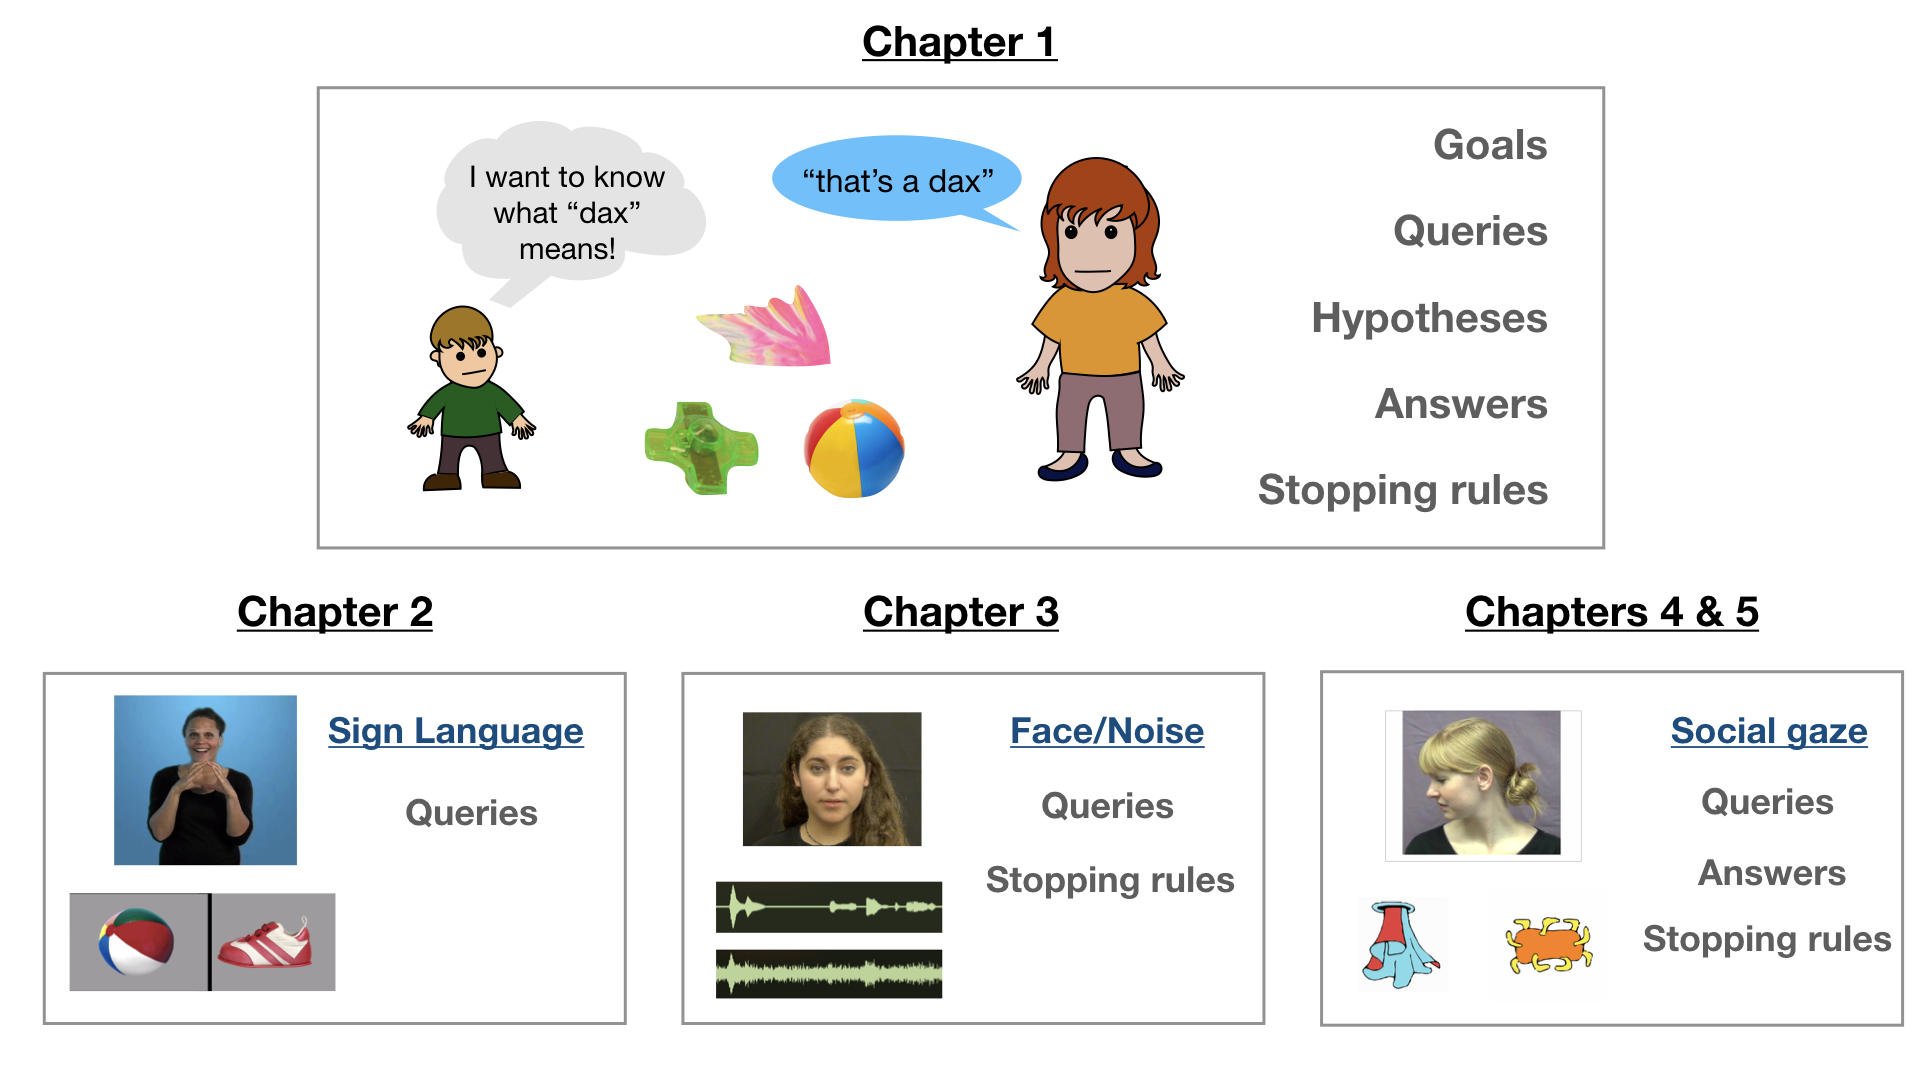
\includegraphics[width=0.9\linewidth]{/Users/ejyoon/Documents/Documents/Research/dissertation/index/chapter_child_rmds/ch0_intro/figs/schematic_overview} 

}

\caption[Schematic overview of the dissertation content.]{The upper panel shows a schematic overview of an integrative framework of polite language understanding based on competing social goals. The lower panels show different studies examining adults' and children's understanding of different component goals (and possible tradeoffs between them) that correspond to each chapter of the dissertation.}\label{fig:schematic-overview}
\end{figure}
\chapter{A goal-based account of polite
language}\label{a-goal-based-account-of-polite-language}

\chaptermark{A goal-based account of polite language}

\section{Introduction}\label{introduction}

Imagine that a stranger on the street approached you and asked: ``I'm
sorry to bother you, but could you tell me the way to the city hall?''
Regardless of your answer, you probably would not feel puzzled or
offended by the way in which the stranger decided to seek information
that he needs. This is in contrast with a different situation where the
stranger said to you instead: ``Tell me the way to the city hall.'' In
such case you would immediately notice the lack of politeness in his
utterance, and your response to him may be negatively affected by the
irritating oddity of the situation. Now imagine another context where a
person was wearing a new, flashy dress, and her friend thought the dress
was hideous. It may actually be more surprising if the friend truthfully
said ``Your new dress is ugly,'' than if the friend decided to lie and
say ``Your new dress is gorgeous!'' But why? Why are people expected to
speak politely, when there are alternative utterances that can convey
information about the world or the speaker's intention more directly
(``Tell me the way'') or truthfully (``Your dress is ugly'')?

Language is a virtuous tool that serves many functions. Through
language, people communicate information about the world, but also form
their social relationships and establish their identity within their
society. On one hand, some theories of language functions describe
language as a transmission device for transferring from a sender to a
receiver information that reflects context or the state of affairs
(Bühler, 1934; Jakobson, 1960; Shannon, 1948). The importance of
informativity is further emphasized in more recent, influential theories
on pragmatics of natural language, which explain how meanings beyond
literal meanings of utterances arise (Grice, 1975; Searle, 1975). On the
other hand, some linguistic theories, especially those with references
to language development, identify social roles of language that people
use to make contact with others and form relationships (Ervin-Tripp,
1967; Halliday, 1975). These theories underscore how linguistic rules
that language users tend to follow represent the norms and structure of
the community using the language (Ervin-Tripp, 1969).

Could polite speech reflect both the informational and the social roles
of linguistic communication? Previous theoretical accounts of polite
speech vary in their focus on informational versus social aspects of
polite language. Some theories view polite speech as reflecting social
rules and norms (Richard J. Watts, Ide, \& Ehlich, 1992), some as
abiding by communicative maxims that people are expected to follow in
conversations, to be both as informative and as affirmative of their
conversational partner as possible (Lakoff, 1973; Leech, 1983), and yet
some others as performing face management, or trying to maintain
interactants' good public self-image or reputation (P. Brown \&
Levinson, 1987).

In this Chapter, I propose that that polite speech highlights both
informational and social uses of language: Polite speech reflects a
principled tradeoff between the informational, epistemic content a
speaker wants to convey (e.g. ``I want you to tell me the way to the
city hall'') and other social concerns, such as prosocial or
self-presentational goal that the speaker wants to express for herself
and others (``I'm not rudely commanding you to tell me the answer, but
making a request in a respectful way''). Thus, my goal is to unify
previous theoretical frameworks in one, goal-driven account of polite
speech. In what follows, I will describe the goal-based account of
polite speech in detail (Part I), and summarize previous models and
theories of polite speech and situate them within the framework of the
current goal-driven account (Part II). Then I will examine empirical
evidence for goal-driven approach to polite speech: In Part III, I will
focus on empirical work on adult production and comprehension of polite
speech which show that adults reason about speaker goals in polite
speech; and in Part IV, I will probe empirical evidence from
developmental work that children's production and understanding of
polite speech advance as they grow older. In doing this I will show that
children's production and comprehension of polite speech is related to
the relative complexity of polite speech based on its goal tradeoff.

\section{Part I: A Goal-based account of
politeness}\label{part-i-a-goal-based-account-of-politeness}

What does it mean to speak politely? Common instances of polite speech
that occur to one's mind probably include the simplest politeness
markers, such as ``please,'' ``thanks,'' and ``sorry.'' More complicated
examples would involve ways in which, for example, a person make a
request: under normally conceivable circumstances, it would certainly be
more polite to ask ``Would it be too much trouble to ask you to complete
this survey when you're not too busy?'' than to say ``Do this survey
now.'' The word ``polite'' can sometimes carry a negative undertone in
its meaning, as in ``she was just being polite,'' which is likely to
mean the speaker was hiding her genuine beliefs or intentions to make
the listener feel good. From these examples, we can identify a few
characteristics that a polite utterance may exhibit: observance of
social rules, relatively high degree of elaborateness or indirectness,
and dishonesty or disingenuousness in the interest of others' feelings
or reputations.

More formal definitions of the term politeness also reveal common
features that polite speech shows. Cambridge and Oxford Dictionaries
respectively define what it means to be polite: ``behaving in a way that
is socially correct and shows respect for other people's feelings''; and
``courteous, behaving in a manner that is respectful or considerate of
others; well-mannered'' (``Polite,'' 2017a, 2017b). Similar to the
previous examples of polite speech, these definitions suggest politeness
involves (1) observance of social expectations and (2) respect for
others. Boyer (1702)'s The English Theophrastus: of the Manners of the
Age, compilation of texts describing the English life in the early
eighteenth century, identifies a purpose in trying to be polite:
``Politeness may be defined as a dextrous management of our Words and
Actions whereby \emph{men make other people have a better Opinion of us
and themselves} {[}emphasis added{]}.'' Thus, according to the
Theophrastus definition, speakers speak politely in order to boost the
self-images of the interactants (both the speakers themselves and their
addressees).

These common themes of politeness have been identified by previous
theoretical accounts of polite speech (reviewed in detail in Part II).
But each of the accounts only focused on certain aspects of polite
speech but disregarded others, and their explanations for politeness
have been viewed as largely disparate. Here I make a unification
proposal, where these existing approaches to polite speech can be united
under a single goal-based account of polite speech.

I propose that polite speech reflects a tradeoff between different
communicative goals, three of which I describe here\footnote{I do not
  intend to argue that this list of goals or their definitions are
  exhaustive; I come back to the possibility of other relevant speaker
  goals in Conclusion.}: informational, prosocial, and
(self-)presentational. \emph{Informational goal} has to do with the
speaker's desire to convey the most accurate information in the most
efficient manner. \emph{Prosocial goal} is about the speaker's desire to
retain the listener's acceptable self-image as a decent individual and
as a reputable member of society. \emph{Presentational goal} reflects
the speaker's desire to present the speaker herself in a good light, to
appear to be a kind and helpful individual. Below I describe each goal
in more detail.

\subsection{Informational goal}\label{informational-goal}

A speaker's informational goal, i.e.~to prioritize information transfer
in communication, may involve two closely related notions: informativity
and truthfulness. Informativity is the notion of conveying the intended
meaning in the most efficient and precise manner possible. The idea of
informativity here is similar to Grice (1975)'s notion of cooperativity:
A speaker will cooperatively choose utterances such that the listener
can understand her intended message. Thus, the current notion of
informativity that I adopt will encompass the whole Cooperative
Principle (CP) that Grice posited (``Make your contribution such as
required by the purposes of the conversation at the moment''), and
especially the Maxim of Quantity (``Make your contribution as
informative as is required''), though Maxims of Relevance (``Be
relevant'') and Manner (``Be perspicuous''; i.e.~be brief, orderly, and
unambiguous) can also be relevant to the notion of informativity as I
discuss in this Chapter.

The idea of informativity has been formalized in probabilistic
(Bayesian) models as a utility function of a speaker with particular
goals in mind. The ``rational speech act'' (RSA) theory of language
understanding (see N. D. Goodman \& Frank (2016) for a review) assumes
that listeners expect speakers to aim to be helpful yet parsimonious,
choosing their utterances approximately optimally based on a
communicative goal (e.g., inform the listener) and interpret an
utterance by inferring what the helpful speaker meant based on the
utterance and any other relevant information about the world. The theory
defines a standard, informative utility as the amount of information a
literal listener (\(L_0\)) would still not know about world state
(\(s\)) after hearing a speaker's utterance (\(w\)):

\[U_{epistemic}(w; s) = ln(P_{L_0}(s | w))\]

where the utterance choice is approximately rational (i.e., in
proportion to the expected utility gain) and \(w\) is chosen from a set
of alternative, relevant utterances.

For example, if Bob asked Alice ``How was my cookie?'' and Alice said to
Bob ``It was good,'' with only the goal to be informative in mind, Bob
would think that Alice was being maximally informative by using the word
``good'' instead of another relevant, stronger word such as ``amazing,''
and infer that Ann meant ``good but not amazing'' because otherwise Ann
would have used the word ``amazing'' instead.

I note here that Ann's speech act could be analyzed as having observed
the Gricean Maxim of Quantity, by making her utterance maximally
informative, and Bob's inference as being based on such assumption that
Ann's utterance is as informative as is required to meet Bob's needs.
But as the comparison between the former goal-directed analysis and this
latter maxim-based analysis may reveal, the maxim-based account is
difficult to formalize (Hirschberg, 1985) whereas the goal-directed view
allows for quantitative account of factors contributing to the
linguistic phenomena at hand (N. D. Goodman \& Frank, 2016). From here
on, I take the goal-directed view rather than the Gricean maxim-based
view of the speaker; thus, analyses of speakers and their utterances
will be based on speakers' communicative goals to convey information,
etc., rather than their observation or violation of Gricean maxims.

Informational goal can also involve truthfulness: the meaning that
accessed by the listener should match the true state of the world as
closely as possible. In other words, the speaker will want to convey
what is true (to the extent of her knowledge), not what is false. For
example, if Bob baked some cookies and they tasted terrible, and Alice
had the goal to be truthful, she would want to convey what matches the
true state of the world as closely as possible (``Your cookies tasted
terrible''). On the other hand, if Alice remarked to Bob about his
cookies ``Your cookies tasted good,'' with goal to be informative and
truthful, the true state of the world must be such that Bob's
presentation was truly good (but probably not amazing, because otherwise
Alice would have said that it was amazing), and not bad or terrible.

As for when speakers decide not to tell the truth, there is a difference
between violating versus flouting of truthfulness (which Grice also
discusses; see Grice (1975), p.~49, 53). Flouting involves contradicting
common knowledge shared between the speaker and listener about the true
state of the world, such that the listener notices that the utterance
meaning does not match the true state. For example, after Alice and Bob
together watch a movie that was obviously gory and disturbing to both of
them, if Bob says ``well, that was a really happy, fluffy movie!'' then
his utterance would be flouting truthfulness goal, and Ann would
recognize Bob's utterance as an ironic one. On the other hand, violating
truthfulness does not hold assumption of such common knowledge of the
true state of the world, and thus the listener may not notice the
mismatch between the utterance meaning and true state of the world,
although the listener can potentially access it through other means
(e.g.~realizing that the speaker had reasons to lie). Here I will mainly
focus on violation, not flouting, of truthfulness, for example when
speakers tell white lies (i.e., when the speakers do not intend that the
listeners know what the truth is).

Speakers' informational goal to be informative and truthful may
encompass communicative cooperation in both locutionary and
perlocutionary senses. A locutionary goal deals with conveying the
intended meaning of the utterance within a conversation, whereas a
perlocutionary goal involves achieving the speaker's ultimate goals
toward the listener (Attardo, 1997). What could be an informational goal
in its perlocutionary sense? In being truthful, speakers may ultimately
want to maintain their moral obligation to tell the truth to others.
This obligation is in line with Western philosophers' argument
throughout the history that it is morally wrong to lie (Augustine, 1952;
Kant, 1949), although there have been debates on whether the degree of
wrongness may depend on context (e.g., if the speaker was telling a
white lie; Sweetser, 1987). For example, if Alice said to Bob ``Your
cookies were good,'' Alice's locutionary goal would be to convey to Bob
her intended meaning that his presentation was good (but perhaps not
amazing), whereas her perlocutionary goal would be for Bob to think that
the presentation was good, which was (apparently) the truth; Alice
thereby upholds her moral obligation to tell the truth to Bob. Alice's
goal to be truthful, then, is achieved in both locutionary and
perlocutionary senses.

Besides an informational goal, a speaker may also want to address
concerns that are social in nature: having to do with interacting and
maintaining good relationships with other people. Below I describe two
related but different goals that speakers may want to accomplish for
social reasons: prosocial and presentational.

\subsection{Prosocial goal}\label{prosocial-goal}

A prosocial goal involves the speaker's desire to to follow social norms
and make others feel happy and respected. Speakers can try to accomplish
the prosocial goal in several ways, one of which is social norm
observance: abiding by social norms and expectations. There may be
simple rules such as ``say please when you make a request'' or ``say
thanks to express gratitude,'' but sometimes the norms can be more
complex. Speakers should avoid saying utterances that are \emph{too}
polite, to the extent that the utterances become marked and are no
longer considered ``optimally polite.'' For example, a request for
opening a window by saying ``Sorry, could you open that window behind
you? Thanks.'' would be a normal, socially expected way to make the
request; but a request such as ``I'm so terribly sorry to bother you
with this irritating request, but if you don't mind, would you care to
open that window behind you, only if it's not going to be too much
trouble for you?'' would be a signal to the addressee that something in
the situation is odd and marked; either that the request involves a
higher cost than is normally expected for opening a window, or the
speaker is unusually afraid of incurring a debt to the addressee, etc.
This principle of social norm observance is then parallel to Grice's
Cooperative Principle, in that the CP outlines normative expectations
for a speaker who wants to convey information as efficiently as
possible, whereas the current principle of social norm observance deals
with normative expectations for a speaker who wants to maintain social
order. Thus, if the CP is a principle of information transfer, social
norm observance is a principle of social order. Both principles call for
unmarkedness of utterances, and when the utterances are marked due to a
violation of its rules, then the listener will try to infer reasons for
such violation.

Speakers may also try to be prosocial through face management.
\emph{Face} is a notion introduced by Goffman (1967), and represents an
individual's publicly manifest self-esteem. He argued that people
perform interpersonal rituals whereby face maintenance is a fundamental
condition of the interactions. Goffman identified two kinds of faces
that people want to maintain: \emph{positive face}, or the want for
solidarity or approval from others, and \emph{negative face}, or the
want to be free from imposition. Interactants will always want to
preserve each other's face, and so potential face threats will somehow
have to be modified. P. Brown \& Levinson (1987) suggested that a
strategy for such facework is politeness, which they defined as
deviation from Gricean informativity (described in detail in Part II).

For example, a request such as ``You couldn't possibly pass the salt,
could you?'' would be an example of negative politeness strategy (i.e.~a
strategy to save negative face; P. Brown \& Levinson, 1987, p. 136) as
the speaker is being pessimistic about the compliance of her request and
not assuming that the listener has to be willing or able to do any acts
predicated of him. On the other hand, utterances that emphasize the
common ground between the speaker and listener (i.e.~that the speaker
and listener share the same goals, values, knowledge, etc.), and address
the fulfillment of the listener's want are positive politeness
strategies; for example, ``What a beautiful vase this is! Where did it
come from?'' (P. Brown \& Levinson, 1987, p. 103) saves the listener's
positive face by attending to the listener's wants and interests. When
face management is in conflict with informational goals, the meaning of
utterance would differ depending on which goal the speaker decided to
prioritize. As described earlier, if Ann said to Bob, ``Your
presentation was good,'' and she wanted to prioritize informational
goals only, then her utterance would indicate that Bob's presentation
was truly good (though perhaps not amazing). However, if Ann spoke with
a prosocial goal to save Bob's face and wanted to boost his self-image
instead, then Bob's presentation actually could be bad rather than good.

\subsection{Presentational goal}\label{presentational-goal}

Language also reflects a speaker's goal to present themselves in a good
light, thereby saving the speaker's own face. This last goal is related
to the informational and prosocial goals previously described, in that
speakers must be mindful of the listener's want to be informed or to
maintain his positive self-image, but instead of actually \emph{being}
maximally informative or prosocial, presentational goal concerns
\emph{appearing} to care about these goals. Thus, a speaker may engage
in a recursive reasoning about a listener who thinks about a speaker who
wants to be informative and/or prosocial, and then can produce
utterances to make the listener \emph{think} that the speaker is being
informative, being prosocial, or both of those things.

The pursuit of self-presentational goal can often lead to the same
outcome as the pursuit of informational or prosocial goals. For example,
if the listener asks for feedback about his performance that was truly
good, all three goals - namely, informational goal to give the listener
accurate information, social goal to make the listener feel good, and
self-presentational goal to appear to be an informative and kind speaker
- align such that they can lead to production of similar utterances,
such as ``Your talk was amazing.''

There are however situations in which each of the three goals has
different consequences: if the listener's performance was truly bad,
then the speaker would need to consider which goal to prioritize. The
pursuit of informational goal would lead to informative but harsh
utterances such as ``Your talk was bad.'' Prosocial goal would yield
nice-sounding but misleading utterances such as ``Your talk was great.''
On the other hand, a speaker who wanted to \emph{appear} to be
informative and kind at the same time may produce a different utterance,
such as ``Your talk wasn't bad,'' or ``It's hard to give a good talk.''
The speaker could thereby convey to the listener that there were reasons
she could not produce a simpler, more direct utterance, and make the
listener think that his performance was probably unexciting but the
speaker was too kind to say it explicitly (see Chapter 4 for the formal
definition and more detailed description of the presentational goal).

\section{Part II: Previous theoretical accounts of polite
speech}\label{part-ii-previous-theoretical-accounts-of-polite-speech}

In Part II, I aim to (i) describe different classes of theoretical
approaches to the understanding of polite speech; (ii) for each class,
explain how the approach can be situated within the current proposal for
the goal-based account for polite speech; and (iii) discuss what
advantages the goal-based account can offer beyond the existing
approaches. Summary of prominent theories and their implications within
goal-based framework can be found in Table~\ref{tab:litRevTable}.

\newpage

\blandscape
\begin{table}[t]

\caption[Review of existing theories of polite language]{\label{tab:litRevTable}Summaries of previous theoretical approaches to polite speech and their implications within the current goal-based framework.}
\centering
\resizebox{\linewidth}{!}{
\begin{tabular}{>{\raggedright\arraybackslash}p{3cm}>{\raggedright\arraybackslash}p{5cm}>{\raggedright\arraybackslash}p{8cm}>{\raggedright\arraybackslash}p{8cm}}
\toprule
\textbf{Politeness as:} & \textbf{Theories offered by:} & \textbf{Summary} & \textbf{Advantage of goal-based framework}\\
\midrule
Observance of communicative maxims & Lakoff (1973); Leech (1983) & Polite speech is governed by conversational rules and principles, that are complementary to Gricean Cooperative Principle (Grice, 1975) & Gradient degree of goal tradeoff can be represented, instead of binary observance of different maxims\\
Strategy for facework & Brown \& Levinson (1987) & Speakers produce polite speech to save interactants<d5> face (positive and negative) & Clearer distinction between notions of truthfulness and informativity becomes possible, which then allows more precise analysis of goal tradeoffs\\
 & Spencer-Oatey (2000) & Speakers try to preserve interactants' face and sociality rights & \\
Social rules and norms & Watts (1989); Locher \& Watts (2005); Watts et al. (1992); Watts (2003) & Speakers use speech to perform relational work (not only face-work); speakers produce im/polite (marked) utterances and politic (unmarked, normative) utterances & No distinction between polite vs. politic utterances is necessary\\
 & Fraser \& Nolen (1981); Matsumoto (1988); Ide (1989); Mao (1994) & Speakers want to fulfill societal obligations & Facework and social obligation do not have to be mutually exclusive\\
\addlinespace
Model of game theory & Franke \& Jager (2016); Pinker et al. (2008); Van Rooy (2003); Quinley (2011) & Speakers use polite speech to get what they want while allowing for plausible deniability, or to communicate their good intentions (while incurring cost) & Self-interest is formalized as arising from recursive reasoning that is based on genuine other-oriented goals\\
\bottomrule
\end{tabular}}
\end{table}
\elandscape

\subsection{Politeness as observance of communicative
maxims}\label{politeness-as-observance-of-communicative-maxims}

One approach to polite speech is largely based on the Gricean
perspective, and claims that conversation is driven by general
communicative principles, and politeness is a maxim (or made up of
maxims) that accompanies other principles. Whereas Grice focused on
principles that speakers follow to make their speech maximally ecient
for information transfer, he also noted: ``There are \ldots{} all sorts
of other maxims \ldots{}, such as `Be polite,' that are normally
observed by participants in talk exchanges'' (Grice, 1975, p. 47).
Searle (1975) discussed conditions of performing indirect speech acts
(e.g. ``Can you pass the salt?'') for which, he claimed, ``politeness is
the chief motivation'' (p.~76). Thus, Grice and Searle both identified
politeness as a driving factor in communication, but the concept of
politeness was largely undeveloped at the time.

The communicative maxim approach for polite speech expanded with
proposals for conversational rules and principles that govern polite
speech. Lakoff (1973) suggested a set of rules (``Don't impose,'' ``Give
options,'' ``Be friendly'') that underlie utterances that are polite,
and thus deviate from directly expressed meanings. Leech (1983)
developed a similar proposal to Lakoff's in greater detail, proposing
Politeness Principle (PP), which is complementary to the Gricean CP.
Leech argued that the PP, like the CP, can be subclassified into more
specific maxims: Maxims of Tact, Generosity, Approbation, Modesty,
Agreement, and Sympathy. The primary postulate of the PP is that
interactants prefer to express polite beliefs, which are beliefs that
are favorable to the other person (and/or unfavorable to oneself). For
example, Approbation Maxim states that a speaker observing the PP will
minimize dispraise, and maximize praise, of the other person (e.g.
``Your dress looks gorgeous!''), whereas Modesty Maxim states that a
speaker will minimize praise, and maximize dispraise, to the speaker
herself (e.g. ``This is just a small gift, but I hope you like it''
downplaying the value of the gift). Gu (1990) proposes addition of
``Balance Principle'' to the set of politeness maxims, where favors from
A to B are balanced by favors from B to A, such that the PP can function
to maintain social equilibrium.

Based on the goal tradeoff framework, it becomes possible to translate
different politeness maxims and their utterance predictions in terms of
the set of goals (informational, prosocial and presentational) that I
argue for. The Approbation Maxim expects a speaker to produce utterances
that minimize dispraise such as ``you could be more careful.'' This
utterance can reflect that the speaker has: (1) informational goal to
convey that the listener \emph{should} or even \emph{must} be more
careful; (2) prosocial goal to not criticize explicitly (e.g., say ``you
are so careless''), which may hurt the listener's feelings; and (3)
presentational goal to appear as someone who cares about both of these
goals mentioned.

The Maxim of Agreement, a different maxim proposed by Leech, can also be
re-interpreted in terms of goal tradeoffs. The Maxim of Agreement
predicts speakers to ``mitigate disagreement by expressing \ldots{}
partial agreement'' (Leech, 1983, p. 138), for example in a conversation
where A says ``The book is tremendously well written'' and B follows,
``Yes, well written as a whole, but there are some rather boring
patches, don't you think?'' If we construe \emph{agreement} as approval
of one's opinion by otherss, which can boost one's self-image (face),
then we can also translate the speaker B's desire behind her utterance
as reflecting: (1) presentational goal to appear to agree with A
(``True''); and (2) informational goal to convey some disagreement
(``but\ldots{}''). In this way, the goal tradeoff framework can help
unify interpretation of utterances based on just a few underlying goals,
instead of relying on many distinct categories of maxims to classify
each utterance as its unique kind.

\subsection{Politeness as strategy for
facework}\label{politeness-as-strategy-for-facework}

Another approach to analysis of polite speech that has been highly
influential is the model of politeness as face management, developed by
P. Brown \& Levinson (1987). The model is primarily based on the concept
of face (Goffman, 1967) that deals with an individual's public persona
(introduced earlier in Part 1). P. Brown \& Levinson (1987) take a
strategic approach to politeness, and focuses on strategies that
speakers employ in order to avoid, redress, or mitigate threats to face
(either the addressee's or the speaker's own). Like the communicative
maxim approach, P. Brown \& Levinson (1987)'s account also start at the
assumption of the Gricean CP, and attribute the cause of a speaker's
deviations from the CP to the speaker's desire to be polite. Thus, given
a speaker's desire to save face, the more an utterance deviates from
maximal informativity, the more ``polite'' (face-saving) the utterance
will be.

Within the goal-based framework, it can be said that P. Brown \&
Levinson (1987) recast the notion of a cooperative speaker as one who
has both an informational goal to improve the listener's knowledge state
as well as a social goal to minimize any potential damage to the
hearer's (and the speaker's own) face. With the idea of these
conflicting goals, Brown and Levinson's theory is conceptually closest
to the current proposal among all theories to be discussed.
Specifically, they primarily focus on the conflict between goals of
social face management and epistemic informativity. For example, by
saying ``Can you please open the window?'' instead of ``Close the
window,'' the speaker decides to sacrifice informativity (i.e.~maximally
efficient transfer of the intention for the addressee to open the
window) in order to save the addressee's negative face (i.e.~freedom
from imposition or order from others). Another example of negative
politeness (i.e.~strategy to save negative face) is a speaker fronting
his gift-giving by saying ``This is just a small gift'' in order to
emphasize that the listener is not incurring too much debt to the
speaker and thus not being imposed a burden to return the favor. On the
other hand, positive politeness or act of saving positive face can be
exemplified by utterances that emphasize approval of the listener's
interest or performance, e.g. ``What a fantastic garden you have!'' (P.
Brown \& Levinson, 1987, p. 104).

One drawback in P. Brown \& Levinson (1987) is that key elements
required for analysis of speakers' goals or intended meanings are
ambiguous and difficult to formalize. The core assumption of Brown and
Levinson's analysis is that deviations from Gricean maxims (that
prioritize the match between the literal and intended meanings) lead to
increase in politeness. In order to estimate the degree to which
speakers try to be polite, there should be a way to measure the degree
of deviation from the Gricean maxims (i.e.~the degree of mismatch
between the utterance surface meaning, intended meaning, and true state
of the world; see Section 1 for how these factors can be formalized
e.g.~in RSA). However, Brown and Levinson do not provide a way to
formalize the literal or intended meaning or the state of the world. For
example, it is unclear how much deviation from the Gricean maxim(s)
occurred when a speaker produced an utterance such as the example
previously mentioned: ``What a fantastic garden you have!'' Since the
authors do not provide the true state of the world (i.e.~how beautiful
the garden actually was in the speaker's opinion), it is difficult to
define or quantify the speaker's effort for politeness or the cost of
face threat the message would have involved given an alternative
utterance (``It is a mediocre garden you have.'') A clearer
identification of the true state of the world, the speaker intended
meaning, and the set of relevant alternative utterances, and a way to
formalize these elements, will help with quantificational analysis of
polite utterances.

Another issue is in P. Brown \& Levinson (1987)'s construal of face,
namely that it is difficult to distinguish between the speaker's desire
to save the listener's face and their want to boost the speaker's own
self-image. For example, by saying ``What a fantastic garden you have!''
the speaker is not only making the listener feel good, but also
presenting the speaker herself as someone who is generous and likes to
compliment others. Brown and Levinson's analysis did not explicitly
differentiate the other-oriented versus self-oriented face-saving goals,
but they can have important implications for situations in which the two
goals lead to different choices. For example, if a speaker simply wants
to save the listener's face, the speaker may produce an utterance that
is unambiguously nice (``Your dress is gorgeous!''). However, if the
speaker wants to inform the listener of some harsh truth but still wants
to save his own face and \emph{appear} to the listener to care about her
feelings, the speaker might say something that is more indirect and
vague, like ``I thought your other dress was very beautiful, how about
wearing that to the party?'' Distinguishing the other-oriented and
self-oriented social concerns thus will help make more precise
predictions for what speakers say and how listeners understand polite
utterances.

Spencer-Oatey (2000) put forward another theory based on Goffman's
notion of face; it is a more general model of rapport management, or
management of interpersonal relations, distinguished from face
management as proposed by Brown and Levinson. Spencer-Oatey challenges
Brown and Levinson's distinction between positive and negative face, and
argues that the former involves the concept of face, or the positive
social value claimed by a person, whereas the latter does not concern
face but rather what she calls ``sociality rights,'' or a person's
entitlements in interactions with others. She then further proposes that
face management and sociality rights management each has both personal
components (concerning self-esteem and individual identity) and social
components (concerning social role and entitlements within relations
with others). Spencer-Oatey then largely focuses on speakers' attempt to
balance between general epistemic goals and both face management and
social expectations. Thus, in saying ``This is just a small gift, but I
hope you like it'' the speaker may not only be concerned about the
speaker's and the listener's faces as individuals but also the
conventional social obligations associated with gift-giving that the
speaker and listener are expected to follow through. However, similar to
Brown and Levinson's analysis, Spencer-Oatey's analysis is limited in
that it does not identify or formalize the epistemic knowledge (the
speaker intended meaning and true state of the world) behind utterances,
making it difficult to quantitatively analyze the goal tradeoffs.

\subsection{Politeness as social rules and
norms}\label{politeness-as-social-rules-and-norms}

Another set of theories for polite speech relies on the notion that
politeness deals with following social norms and expectations. One line
of theory argues for the need to distinguish between marked, strategic
polite behaviors versus unmarked, normative ``politic'' behaviors.
Richard J Watts (1989) defines ``politic'' behavior as
``socio-culturally determined behavior directed towards the goal of
establishing and/or maintaining in a state of equilibrium the personal
relationships between the individuals of a social group, whether open or
closed, during the ongoing process of interaction.'' For example, ``May
I open the window behind you?'' will be a normative, politic statement
if used in a formal setting or said to a stranger, but can be considered
marked, overly polite statement when said to a close family member.

Richard J. Watts et al. (1992) posited that examples of polite speech in
Brown and Levinson's work, such as honorifics or indirect speech acts,
will be considered ``polite'' only if they go beyond their normal usage
as socio-culturally constrained forms of politic behavior. For example,
according to Watts, responding to an offer ``Would you like some more
co↵ee?'' by nonsaliently saying ``Yes, please.'' (Richard J Watts, 2003,
p. 186) should be considered a politic behavior. On the other hand, if
the response is instead ``Yes, please, that's very kind, coffee would be
wonderful.'' Culpeper (2011) is considered to be polite as it is
``perceived to go beyond what is expectable'' (Richard J Watts, 2003, p.
19). Based on these observations, Locher \& Watts (2005) claim that, a
better approach than Brown and Levinson's ``facework'' to encompass all
degrees of polite speech will be a larger ``relational work'' that
considers all-ranging levels of politeness from marked im/polite to
unmarked politic utterances.

Watts and colleagues' claim can be re-framed as calling for the need to
consider wide-ranging informational-social tradeoffs. Watts' distinction
between politic versus polite speech lies in whether the addressee
recognizes and pays attention to the divergence between speakers'
informational and social goals, as revealed by the discrepancy between
literal versus intended meaning, and tries to infer the intended
meaning. For politic utterances, the mismatch between literal and
intended meaning is unmarked and thus remains unnoticed; For polite
utterances, the mismatch is salient and the listener is called to pay
attention to the reason for that mismatch, and to infer what a speaker
was truly trying to say or what the speaker truly believed (i.e.~the
true state of the world).

One benefit of the current goal-based account over Watts et al.'s claim
is that there is no need to classify different kinds of polite speech as
different categories (polite vs.~politic). Rather, by observing how
subtle changes in the literal meaning, intended meaning, or the true
state of the world can lead to changes in a speaker's inferred goals or
evaluation of politeness, one can examine the phenomenon as a whole.
Watts et al.'s theory makes it rather difficult to know exactly what
utterances count as polite vs.~politic; for example, should the
utterance ``This is just a small gift, but I hope you like it'' produced
in a gift-giving act be considered politic or polite? The goal-based
framework obviates this need and quantifies the relative degree of
politeness in terms of goal tradeoff.

Other theorists have focused on speakers' attempt to abide by societal
obligations and expectations, explicitly distinguishing between their
accounts and ``strategic'' approach to politeness based on individual
goals (e.g., P. Brown \& Levinson, 1987). Fraser \& Nolen (1981) put
forth an account for politeness based on the idea of ``conversational
contract'' (CC), which posits that interactants bring a set of rights
and obligations to the conversation. Observance of these obligations,
according to these authors, are not strategic but rather ``getting on
with the task in hand in light of the terms and conditions of the CC''
(Fraser, 1990, p. 233). Critiques of polite speech analysis based on
facework by sociolinguists (Ide, 1989; Mao, 1994; Matsumoto, 1988)
assert the importance of considering speakers' desire to fulfill
societal obligations. They go against Brown and Levinson's notion of
``negative face'' as it is heavily loaded with the assumption of
individuality as opposed to group identity, which especially becomes
prominent in East Asian cultures and languages. Thus, they may argue
that an utterance such as ``This is just a small gift, but I hope you
like it'' in East Asian cultures may not reflect an attempt to save the
listener's negative face, but to follow convention based on their
assigned role (e.g.~within a hierarchical social structure).

The proponents of social obligation approach for politeness focus
primarily on speakers' prioritization of observance of social norms over
informational goals. This approach rejects the assumption of
universality of face management principles claimed by Brown and
Levinson, and argues that in some cultures the need for face-work
(especially for individuality) may be weak or non-existent. Instead, a
speaker may desire to follow and reinforce social norms and
expectations, and decide how to balance between that desire and the goal
to transfer information. For example, if a professor is to accompany his
long-time mentor to a restaurant, when it comes to time to pay, the
professor may say ``I insist, you should let me pay for this - please
treat me next time'' despite thinking that he doesn't actually want to
pay the bill, because it is more important to hide his genuine
intentions to abide by what is expected of him as as a lower-status
individual.

The goal-based framework aims to simultaneously acknowledge the
importance of these theories identifying more subtle cases of politeness
and unify them with the work for face-saving strategies (e.g., P. Brown
\& Levinson, 1987) they largely argue against. Whereas the social
obligation theories attempt to reject the facework-based accounts of
polite speech, the current proposal is that speakers consider both
social obligation and facework as potentially important social goals,
and try to balance between these social goals and epistemic goals to
convey their message. Thus, instead of presuming mutual exclusivity of
speakers' goals either to save face or to abide by social rules, the
goal-based framework instead assumes that both goals can apply
simultaneously, to different degrees depending on the cultural or
conversational context.

\subsection{Politeness in the game-theoretic
approach}\label{politeness-in-the-game-theoretic-approach}

Finally, there have been recent attempts to analyze polite speech from a
game-theoretic perspective, which assumes that individuals interact with
each other in an effort to achieve their own goals. A few proponents of
game-theoretic approach have analyzed indirect speech as a whole,
viewing polite indirect utterances as a subset. Franke \& Jäger (2016)
argue that indirect speech used for demands results in greater
likelihood of compliance from the other party, as indirect speech
suggests higher stakes for the listener in case the speaker's wants are
not fulfilled. For example, a mobster who is trying to take protection
money from a restaurant owner could pose a veiled threat by saying:
``Your little daughter is very sweet. She goes to the school in Willow
Road, I believe'' (Franke \& Jäger, 2016, p. 19). This indirect speech
is used to communicate that the restaurant owner's stakes are high
because his daughter can get hurt if he does not pay the money, whereas
mobster's stakes are low because he is free to do whatever he wants in
the neighborhood. Franke \& Jäger (2016)'s account thus focuses on the
reasons to be indirect to send the informational message more
effectively in the interest of the listener's observance of the
speaker's wants, though the scope of their explanation does not
explicitly cover polite speech.

Addressing a broader set of indirect utterances, Pinker, Nowak, \& Lee
(2008) describe three possible reasons for speaking indirectly: allowing
for plausible deniability and thus preventing (legal) responsibility for
the intended meaning (``Ocer, is there some way we could take care of
the ticket here?''), avoiding emotional costs of mismatch (such as
awkwardness) in perceived relationship between speaker and listener, and
generating common reference point that is qualitatively different from
direct literal meaning even when the intended meaning is clear to the
interactants (``Would you like to come up and see my etchings?'').

Other game-theoretic accounts addressed polite indirect speech
specifically, highlighting its rationality despite its potential cost.
Van Rooy (2003) argues that polite utterances are costly ``handicaps,''
which incur a social debt and reducing the social status of the speaker,
but which are rationally used to communicate good intentions to the
addressee. Quinley (2011) observes that politeness is a form of ``trust
game,'' where making a polite request is rational when assumptions of
reputation or observation are in place over multiple iterations of
conversational turns.

Game-theoretic approach is similar to the current goal-based approach in
that the theory is very much built on the notion of tradeoff of goals,
but differs in that it is ultimately focused on the speaker's goals for
the self. In game theory, a speaker's informational goals are centered
around informativity, or effective transmission of the message, to
ultimately gain the desired compliance from the other party (Franke \&
Jäger, 2016). Similarly, a game-theoretic speaker's social goals involve
face management, but less of the intent to save the listener's face and
more to save the speaker's own face, to avoid being held responsible for
disobeying the law or disrespecting someone (plausible deniability) and
to prevent high emotional costs misunderstanding common knowledge
assumed between speaker and listener (Pinker et al., 2008). The current
proposal differentiates between speakers' interest oriented toward
others (i.e., a genuine desire to inform others or save others' face),
and interest towards the speakers themselves (e.g., a desire to
\emph{appear} to be a particular way). I formalize the self-interest
based on a recursive reasoning about the other-oriented goals: Speakers
reason about listeners who imagine speakers to be genuinely informative
or kind, and then the speakers produce utterances that can portray
themselves to be such helpful individuals.

\section{Part 3: Empirical work on polite speech in
adults}\label{part-3-empirical-work-on-polite-speech-in-adults}

In previous sections, I have recapitulated previous theoretical
perspectives to make a unifying proposal that speakers consider
tradeoffs between informational and social goals (e.g., prosocial,
self-presentational). In this section, I review empirical evidence from
adult interpretation, evaluation and production of polite speech that
show their consideration of speaker's informational and social goal
tradeoff.

\subsection{Interpretation of polite
speech}\label{interpretation-of-polite-speech}

Empirical findings show that adults' interpretation of polite utterance
meanings is based on the epistemic-social goal tradeo↵ considered by the
speaker. For example, people's interpretation of seemingly irrelevant,
ambiguous utterances reveal that listeners pay attention to the
epistemic-social tradeoff, attributing politeness as a strong reason for
apparent irrelevance. T. Holtgraves (1998) examined interpretations of
replies to someone asking for an opinion on some performance that he
just gave (e.g. ``What did you think of my presentation?''), where the
replies seemingly did not directly address the questions and involved
relevance violations (``It's hard to give a good presentation''). The
author found that people often assign face-threatening meaning to the
indirect reply. Additionally, people spent longer coming up with an
interpretation when the true state was positive (the addressee actually
gave a good presentation) or when the literal meaning of the reply was
in the positive direction (``It's easy to give a good presentation''),
which thus made face management an unlikely goal. These findings overall
indicate that people identify face management as a key motivation for
violating the informativity goal, and struggled when face management was
no longer a valid reason for violation of the goal to be informative to
the listener.

Another prominent example of polite speech interpretation in line with
the idea of the speaker's goal tradeoff consideration comes from
empirical work on cancellation of pragmatic inferences that are normally
in force in non-face-threatening, low-stakes contexts. People's
inferences change for non-literal meanings of various quantifiers
depending on the presence or severity of face threat toward the
listener. For example, the term ``possibly'' could be used to convey a
probability greater than 0 and up to 1 in its literal sense, but usually
people assume that it denotes a probability that is neither too high nor
too low. This is because people assume that a speaker would use
quantifiers in the most efficient, informative way possible (Grice,
1975), and if the speaker wanted to convey a greater certainty then she
would have used a stronger term, such as ``certainly.''

However, when the situation involves a potential face threat or a high
stake for the listener, the speaker would have a reason to be more
vague, to accommodate for face-saving or plausible deniability. Indeed,
Bonnefon and colleagues found that people interpret the word
``possibly'' as implying a greater likelihood when it is used to
describe a condition of a higher stake (e.g. ``You will possibly suffer
from deafness soon'' or ``Your pain is possibly going to increase'')
than a lower stake (``You will possibly suffer from insomnia soon'' or
``Your pain is possibly going to decrease''; Bonnefon \& Villejoubert
(2006); Pighin \& Bonnefon (2011)).

Similarly, people's interpretation of other quantifier phrases such as
``some'' and ``A or B'' differ depending on the contexts. People usually
endow upper-bounded meanings to ``some'' and ``A or B'' in
non-face-threatening contexts assuming speakers' epistemic
cooperativeness (Breheny, Katsos, \& Williams, 2006; e.g., Huang \&
Snedeker, 2009): ``I ate some of the cookies'' is interpreted to mean
``\ldots{} some of the cookies but not all,'' and ``she ate the cake or
the salad'' to mean ``\ldots{} the cake or the salad but not both.'' In
situations involving face threat, however, people make different
inferences: ``some'' and ``or'' in ``some of the audiences hated your
talk'' and ``We will cut your salary or take away your company car'' are
interpreted in their broader sense (``some and possibly all'' and ``A or
B and possibly both''; Bonnefon et al., 2009; Feeney \& Bonnefon, 2013).
Furthermore, a long pause before the utterance, signaling expectation of
bad news to the listener, heightened the effect for the polite
interpretation of ``some'' (Bonnefon, Dahl, \& Holtgraves, 2015). In
sum, people infer different non-literal intended meanings depending on
the context, since the speaker is expected to focus more towards social,
face-saving goal than towards epistemic goal in the presence of
potential face threats.

\subsection{Evaluation of polite speakers'
intentions}\label{evaluation-of-polite-speakers-intentions}

People's evaluation of strategies to be polite is also based on the
balance of epistemic-social tradeoffs. Clark \& Schunk (1980) showed
that people rate politeness of requests differently depending on how
much the literal meaning of indirect requests would benefit the listener
or reduce the cost to the listener. For example, requests that implied
that the speaker asked for the listener's permission (``May I ask
you?'') were rated as relatively more polite, whereas those requests
that assumed the listener's obligation to reply to the speaker (and
therefore incurs a cost for the listener; ``Shouldn't you tell me?'')
were rated as more impolite. Thus, with the increase of the maintenance
of the listener's face, to be free of imposition or obligation in this
case, relative to the degree of message transfer (i.e.~access to the
intended meaning that was assumed to be constant; e.g. ``Tell me the way
to Jordan Hall''), people's judgment for politeness of requests also
increased.

Interestingly, hints that seem to prioritize face-saving due to its
relatively high degree of indirectness are not always evaluated as most
polite. According to P. Brown \& Levinson (1987)'s rank ordering of
polite strategies, hints (i.e.~indirect speech with meanings that are
``off the record'') are supposedly more polite compared to other
politeness strategies. However, empirical evidence is divided on this
issue (e.g., Pinker et al., 2008; Terkourafi, 2002; Yu, 2011). For
example, Blum-Kulka (1987) found that people rate conventional indirect
requests (e.g. ``Would you mind moving your car?'') as more polite than
direct orders (``Move your car'') or hints (``We don't want any
crowding''). Along similar veins, among possible replies to a question
asking for an opinion on a newly bought dress, people perceive evasive
replies (e.g. ``It seems like clothes are getting terribly expensive'')
to be better than direct utterances (``I don't think it looks very good
on you'') or hints that sound irrelevant (``I'm going to take my
vacation next month''; T. Holtgraves, 1986).

One potential reason why hints and irrelevant remarks are not evaluated
as best politeness strategies is that they focus too much on face-saving
but not information transfer, leading to a poor balance in
epistemic-social tradeoff. Indeed, based on the results of her study,
Blum-Kulka concluded that politeness is ``interactional balance achieved
between two needs: The need for pragmatic clarity and the need to avoid
coerciveness.'' This is in agreement with the current argument that
people consider both the epistemic and social goals as important in
communication, and the balance between these two goals determines what
is optimally ``polite.''

\subsection{Production of polite
speech}\label{production-of-polite-speech}

Adult production of polite utterances reveal their attempt to balance
between epistemic and social goals. Adults spontaneously produce
requests in polite forms that do not convey their message in the most
direct manner (Clark \& Schunk, 1980). Even in situations of conflict,
people try to balance between their desire to convey their message and
desire to control their politeness level; indeed, speakers exhibit
politeness strategies even while arguing, preventing unnecessary offense
to their interactants (T. Holtgraves, 1997).

Sometimes people decide to compromise the level of unambiguity or
certainty that is communicated to the listener due to social reasons. T.
Holtgraves \& Perdew (2016) tested what degree of (un)certainty with
which people would communicate potentially face-threatening information.
They found that if the event referred to was more severe (and therefore
there is greater face threat involved) or if the person whose face was
under threat was the listener (as opposed a third party) participants
used terms with greater uncertainty. Thus, when there is a greater risk
for face threat, and therefore more reason to prioritize face
management, speakers sacrifice information transfer and convey
information more ambiguously.

Situational factors can also lead speakers to prioritize epistemic
versus social goals differently. P. Brown \& Levinson (1987) claimed
that the degree of the face-threat of an act is determined by three
factors: the listener's power status with respect to the speaker; the
degree of social distance between the speaker and the listener; and the
degree of imposition of the act (which may be culturally determined).
Thus, a speaker's attempt to minimize face threat would increase as
these three factors increase in magnitude. If their claim is true,
within the goal-based framework, speakers would prioritize face-saving
goal relatively more as the effect of these sociological factors
increase.

Indeed, empirical evidence suggest that the lower power status of a
speaker, and requests with greater imposition, lead to greater degree of
face-saving (Blum-Kulka, Danet, \& Gherson, 1985; T. Holtgraves \& Yang,
1992; Leichty \& Applegate, 1991; Lim \& Bowers, 1991). For example, in
Lim \& Bowers (1991)'s study, participants were asked to write down
their probable utterances in an imaginary situation involving a
potential face threat and varying degrees of power status of the
listener. The results showed that participants produced more ``tactful''
utterances with more indirect expression of amount of imposition on the
listener (e.g. ``I'd greatly appreciate it if you could write the paper
on behalf of the whole group'') in a scenario involving equal power
between the speaker and listener than when the speaker had higher power
than the listener (e.g. ``I know it's imposing a lot, but you gotta
write the paper again'').

Empirical work on the effect of distance on politeness has been more
inconsistent where some report results that are consistent with Brown
and Levinson's claim that greater distance leads to higher levels of
politeness (T. Holtgraves \& Yang, 1992), while others report the
opposite (Baxter, 1984; R. Brown \& Gilman, 1989). One potential reason
for the inconsistency can be that social distance may be confounded with
affect (i.e.~how much the speaker likes the listener). Nonetheless,
regardless of the directionality, all three variables of power,
distance, and degree of imposition affect speakers' politeness level; in
other words, speakers consider these factors to determine how much
priority they should place on social goal to save the listener's face as
opposed to epistemic goal to effectively convey their message.

In sum, empirical work with adults reveal that people interpret,
evaluate, and produce polite speech in ways that are consistent with the
notion of the epistemic-social goal tradeoff.

\section{Part 4: Empirical work on polite speech in
children}\label{part-4-empirical-work-on-polite-speech-in-children}

In this section, I argue that children's acquisition of polite speech
shows a pattern consistent with the goal-based account: Children show
early competence with polite speech that involves minimal conflict
between speaker goals, and gradually learn to produce and understand
polite speech with more complex patterns of competition between speaker
goals.

\subsection{Rule-based polite speech}\label{rule-based-polite-speech}

Theories on children's sensitivity to conventional rules predict
children's early understanding of simple, rule-based politeness
(i.e.~that does not involve explicit conflict between a speaker's
epistemic and social goals). In the domain of morality, Turiel (1977)
argued that children's early-emerging understanding of social
conventions is primarily based on rules and actions enforced by social
authorities, and then the development of a more flexible
person-orientation occurs throughout childhood. In other words, children
may first start by following simple moral rules such as ``do not cheat''
or ``do not steal,'' but as they grow older they may become more
flexible as they consider more complex circumstances depending on the
needs of the individuals and society involved. In the context of polite
speech, children may show similar developmental trajectory: they could
first faithfully follow rules such as ``say please'' or ``do not lie,''
but as they become more sensitive to intricate demands of different
individuals and contexts, they may start to try to balance between
different goals to satisfy those demands. According to this hypothesis,
children should start to show mastery of rule-based polite utterances,
such as syntactic politeness markers (e.g. ``please'') and conventional
request forms (e.g. ``Can you \ldots{}''), earlier than other more
complex forms of polite speech (e.g.~white lies).

Indeed, children start producing rule-based polite utterances early.
From very early on, parents teach children to be polite by following
normative rituals to say ``please'', ``thank you'', ``hello'' and
``good-bye'' (Gleason, Perlmann, \& Greif, 1984). Children start
producing the simple polite marker ``please'' early at 2.5 years (Read
\& Cherry, 1978) and request forms increase in their variety and
frequency with age (E. Bates, 1976; E. Bates \& Silvern, 1977; Bock \&
Hornsby, 1981; Ervin-Tripp, 1982; Nippold, Leonard, \& Anastopoulos,
1982).

Young children learn to produce these utterances with appropriate levels
of politeness depending on context (Ryckebusch \& Marcos, 2004; e.g.,
Snow, Perlmann, Gleason, \& Hooshyar, 1990). For example, children use
different forms of requests depending on how they are instructed to make
the requests. At three years, children start using different forms of
request when they are instructed to ``tell'' versus ``ask'' an addressee
to give them a puzzle piece (Bock \& Hornsby, 1981). Similarly,
five-year-olds are able to modify requests depending on whether they are
asked to make a request in a nice versus bossy way (Becker, 1986). E.
Bates \& Silvern (1977) showed that even two-year-olds were able to
modify their requests to make them more polite, when they were
instructed to make a request to an old lady and then ask her again ``in
the nicest way possible.'' However, children as old as seven fail to
differentiate the meaning of ``ask'' and ``tell'' when asked Ervin-Tripp
(1977) which suggests that production of context-relevant polite speech
seems to precede the precise, conscious understanding of goals for
speaking politely or impolitely.

Children are also able to adjust the level of politeness based on the
listener age and status. Even at two years, children use a polite form
of request (e.g. ``Can I have\ldots{}'') to an adult but an imperative
form (e.g. ``Give me\ldots{}'') to a peer (Corsaro, 1979; Shatz \&
Gelman, 1973). Children around 2.5 years were to found to use less
polite language with their fathers compared to their mothers
(Ervin-Tripp, Guo, \& Lampert, 1990; Ervin-Tripp, O'Connor, \&
Rosenberg, 1984). These production behaviors are consistent with Brown
and Levinson's prediction that a speaker's need for politeness strategy
will be heightened as the addressee's power status increases.

Furthermore, children make polite requests based on the degree of
imposition of their demands, and respond sensitively to the resistance
to get what they want. By five years, children produce polite speech
that matches the cost of the request they make, using more polite forms
of requests for apparently more costly impositions (Ervin-Tripp et al.,
1990). James (1978) showed that four-year-olds adjusted commands to make
them more polite toward older addressees, whereas when they had to make
requests for getting what they want (which places higher cost on the
speaker if the request is not met) children made the utterances
maximally polite regardless of the listener status. Axia \& Baroni
(1985) showed that seven-year-old Italian children were able to adjust
the polite level of request depending on resistance. Additionally,
children in preschool years and older have been observed to repeatedly
use the word ``please'' in their pleading to resistant mothers and
peers, as strategies to get what they want (Finley \& Humphreys, 1974;
Kyratzis \& Guo, 2001; Wilson \& Wood, 2004). Thus, children use
politeness as a strategy to gain compliance for their goal in the
intended message.

Comprehension of rule-based polite speech also seems to emerge early,
though evidence is more gradual and controversial compared to
production. Initial evidence seemed to suggest that producing a request
with ``please'' is judged to be polite by three years of age (E. Bates,
1976; E. Bates \& Silvern, 1977). However, in a study by Nippold et al.
(1982), this judgment of ``please'' as polite was only replicated
starting at five years of age, but not younger. Furthermore, in the same
study, children did not differentiate between requests that adults
judged to differ in politeness level (e.g. ``Give me some candy,
please'' vs. ``Can you give me some candy, please?'') until seven years
of age. But these initial studies have a few unresolved issues,
including the lack of statistical tests to assess each age group's
performance and lack of systematic manipulation of cues other than
syntax (e.g., voicing or facial expressions). Thus, more evidence is
required to confirm early understanding of conventional polite requests,
but preliminary evidence so far suggests that children start to show
some understanding of these requests before preschool years.

\subsection{Indirect speech}\label{indirect-speech}

Now I turn to children's production and understanding of polite speech
that is more complex than simple rule-based utterances and reflects a
strategic tradeoff between speaker goals. First, what do we know about
children's understanding of indirect speech, where informativity is
compromised for social goals?

Despite the wealth of studies looking at conventional indirect requests
and simple polite markers (``please''), very few studies have looked at
children's understanding of non-conventional indirect requests
(e.g.~hints); there is only limited evidence that comprehension of
under-informative indirect requests is more difficult and is acquired at
a later age than conventional requests. Bernicot and colleagues have
tested French-speaking children's abilities to evaluate implications of
requests for which the intended meaning is distinct from the literal
meaning. Bernicot \& Legros (1987) tested children's ability to
understand implications of directives in different forms: direct
directives (e.g. ``Give me the spade'') versus nonconventional indirect
directives (``I can't make a castle with my hands''). They found that
even by six years, children have difficulty judging what would be an
appropriate reaction by the speaker when the addressee does not comply
with the directives. Bernicot, Laval, \& Chaminaud (2007) found some
evidence that by eight years, children are able to infer appropriate
responses to nonconventional requests in the form of hints. Finally,
ten-year-old children, similar to adults (as shown in Blum-Kulka, 1987),
judge that conventional indirect requests are the ``right thing to say''
more often compared to direct orders or hints, whereas five- and
seven-year-olds do not show this metapragmatic reasoning (Bernicot,
1991).

\subsection{White lies}\label{white-lies}

Next I consider another category of polite utterances reflecting
speakers' goal tradeoff: white lies. Children start producing white lies
early on. Talwar and colleagues have shown the earliest evidence of
white lie-telling in children: They found that the majority of three- to
seven-year-old child participants in their studies told white lies and
stated that an adult ``looks okay for the picture'' even though she has
a conspicuous mark of lipstick on her nose (Talwar \& Lee, 2002), or
lied to a gift-giver about her gift that they actually found undesirable
(Talwar, Murphy, \& Lee, 2007).

Though they produce white lies early, young children's understanding of
goals for production of white lies seems limited. When the participants
in Talwar and colleagues' studies were asked for reasons why they
decided to tell white lies, many stated they did not know why.
Similarly, Italian children of same age group struggled to predict what
the protagonist of a story might say in a situation where telling truth
would not be polite (Airenti \& Angeleri, 2011). Although there was an
increase in the proportion of correct responses with age, even
six-year-olds did not predict the correct response above chance unless
they were given an additional cue to think about politeness-related
reasons. Thus, despite the evidence of early spontaneous production of
white lies in familiar situations, children seem to have limited
understanding of goals behind white lie-telling.

Studies of comprehension and evaluation of white lies show that young
children are more charitable toward prosocial lies compared to other
kinds of lies. Evidence suggests that by four years, children perceive
prosocial lies as better than malicious lies (Bussey, 1999), and they
rate lies as nicer than truths in politeness situations (M. Song \&
Song, 2014). G. D. Heyman, Sweet, \& Lee (2009) observed that 7- to
11-year-old children rated lie-telling more favorably in politeness
situations (e.g.~a teacher gave the protagonist an undesirable gift)
than in transgression situations (e.g.~the protagonist damaged a library
book). This tendency to rate prosocial lies positively increases with
age (Walper \& Valtin, 1992).

Children's favorable perception of white lies tends to depend on their
recognition of speaker goals and reasons for white lie-telling. When G.
D. Heyman et al. (2009) asked participants for explanations of their
evaluation of the protagonist's behavior (telling a lie or truth) in
politeness context, the participants were more likely to rate
lie-telling more favorably and truth-telling more negatively when their
focus was on the impact of the statement on others rather than the
veracity of statements. Studies in other countries have also found that
children in elementary school years view lie-tellers more positively if
the lie is told in a public, face-threatening situation (Ma, Xu, Heyman,
\& Lee, 2011), or is intended to benefit others rather than the speaker
herself (Fu, Heyman, Chen, Liu, \& Lee, 2015). Overall these findings
show children evaluate white lies and blunt truths differently based on
which communicative goal or intention is prominent in the given context.

As they get older, children make more subtle inferential judgments about
implications of white lies, which shows their ability to identify
epistemic and social goals as separate intentions manifested in white
lies. Children become able to differentiate between various traits of a
speaker based on her goal tradeoff decision. Xu et al. (2013) told 7- 9-
and 11-year-old Chinese children stories of lie-tellers and
truth-tellers with either intent of helping or harming the addressee,
and looked at their ratings of benevolence and trustworthiness of the
speaker. The participants rated helpful characters (both lie-tellers and
truth-tellers) as nice and harmful characters as mean; for trust
evaluations, younger children relied more on honesty whereas older
children relied more on the intentions. This finding reveals an
interesting trend in which children of younger ages are more narrowly
focused on the speaker's truth-telling goal, whereas older children
consider the goal tradeoff more holistically and gradually shift their
preference toward the face-saving goal. Indeed, in another study by Xu,
Bao, Fu, Talwar, \& Lee (2010), Chinese children from the same age group
who considered both honesty and politeness issues in evaluating white
lie-tellers tended to tell a white lie more often than those who focused
on only one of the two issues.

\subsection{Summary}\label{summary}

In sum, the development of production and understanding of polite speech
show predicted trajectories based on the currently proposed goal-based
account. A greater degree of conflict or tradeoff between the speaker's
informational and social goals leads to more challenging cases of polite
speech that are more difficult to produce or comprehend. Thus, from
early on, children produce and understand many instances of rule-based
polite speech using simple markers of politeness, involving minimal
conflict between epistemic and social goals. As for indirect speech and
white lies, cases that reflect speakers' decisions based on the goal
tradeoff, younger children before elementary school years show only
limited understanding of motivation behind these more complex
utterances. Finally, school-year children become competent at
identifying reasons for both truth-telling (for epistemic reasons) and
prosocial lie-telling (for social reasons) and making informed
evaluations of speakers based on their tradeoff decisions.

\section{Conclusions}\label{conclusions}

In this Chapter I argued for a goal-based account of polite speech, in
which speakers consider their competing social goals (informational,
pro-social, and self-presentational goals) to speak politely. The
goal-based approach provides a way to unify previous theoretical
frameworks for polite speech, and is consistent with empirical evidence
in adults' and children's production and comprehension of polite speech.

In Chapters 2 through 4, I will present empirical evidence from adults
and children to support the goal-based account of polite speech. Chapter
2 presents a formal model of how polite speech emerges. We explored how
speakers are expected to speak politely in situations where they are
asked to provide feedback for the addressee's performance (e.g., poem
recital). We built a computational model based on the assumption that
speakers should consider goals to be informational, pro-social and
self-presentational in speaking politely (as addressed in Chapter 1),
and we show that our model successfully captures important patterns of
adult predictions for polite speech (e.g., white lies and indirect
speech).

Chapters 3 and 4 examine children's understanding of polite speech. In
Chapter 3, we look at whether 2- to 4-year-old children are able to
understand that speakers account for prosocial goals in their speech, by
examining their evaluation of polite requests (e.g., ``Can you please
pour me more water?''). In Chapter 4, we investigate whether children
reason about tradeoff between different goals (e.g., informativity
vs.~prosociality) by looking at their evaluation of white lies (e.g.,
``Your cookie was tasty'') versus blunt truths (``Your cookie was
yucky'').

The primary goal of this dissertation, then, is to probe whether and how
adults and children reason about polite speech as reflecting competing
goals to be informative, to be kind to others, and to present oneself in
a good light, and tradeoffs between these goals.

\chapter[Children understand social goals behind polite
requests]{\texorpdfstring{Children understand social goals behind polite
requests\footnote{This chapter is submitted and currently under review
  for the 41st Annual Meeting of the Cognitive Science Society, and is
  joint work with Michael C. Frank.}}{Children understand social goals behind polite requests}}\label{children-understand-social-goals-behind-polite-requests}

\chaptermark{Children's understanding of polite requests}

In this Chapter, I start to explore what children understand about
polite speech. Looking at children's polite speech comprehension can
help examine children's pragmatic understanding more generally, and can
be informative for caregivers who want to teach children what it means
to be polite. Even though children start to produce polite speech from
early on, there is little known about whether they understand intentions
behind polite language. In this Chapter, I show that by 3 years,
English-speaking preschool children understand that it is more polite
and nicer (and less rude and mean) to use politeness markers such as
"please" when making requests, and by 4 years, they understand that the
use of these politeness markers indicates that the speaker is more
socially likeable and is more likely to gain compliance from their
conversational partners. This work can help lay the foundation for
future work on children's understanding of polite speech and pragmatic
development more generally.

\section{Introduction}\label{introduction-1}

We use and hear polite speech on a daily basis: polite utterances range
from simple words of apology (``sorry'') or gratitude (``thanks'') to
compliments (``I love your dress!'') and requests (``Can you please open
the window?''). Yet polite utterances are seemingly inefficient and even
misinformative: speakers say ``Can you please \ldots{}'' when it should
suffice to say, ``Open the window.'' These facts are a mystery for
frameworks which describe communication in terms of efficient
information transfer (e.g., Bühler, 1934; N. D. Goodman \& Stuhlmüller,
2013; Shannon, 1948): If language is a tool for transferring
information, speakers should be as efficient as possible in their
communication to prioritize informativity. Nonetheless, everyday
politeness is ubiquitous in everyday language use, and adults tend to
use strategies to be polite even while arguing (T. Holtgraves, 1997).

So why do people speak politely? Linguistic theories assume that
people's utterance choices are motivated by social concerns, framed as
either maxims (Leech, 1983), social norms (Ide, 1989), or listener's
and/or speaker's public identity (\emph{face}; P. Brown \& Levinson,
1987). For example, P. Brown \& Levinson (1987)'s theory predicts that
if a speaker's intended meaning contains a threat to the listener's face
or self-image, the speaker's utterance will be less direct and less
informative. For example, if a speaker considered that saying ``Open the
window'' will give the impression that she is in a position to give
orders to the listener, she could instead say ``Can you please open the
window?'', using a more indirect form of request to give the other
person a sense of autonomy or freedom from imposition (Clark \& Schunk,
1980). Thus, while it may hinder the goal of efficient information
transfer, using polite speech can help the speaker save the listener's
face while simultaneously communicating her own positive social goals
(Yoon, Tessler, Goodman, \& Frank, 2017).

Do children speak politely, and if so, what do they understand about
polite speech? Previous research shows that children begin producing
polite speech early on; They produce ``please'' at 2.5 years (Read \&
Cherry, 1978), and request forms increase in their variety and frequency
with age (E. Bates, 1976; E. Bates \& Silvern, 1977; Bock \& Hornsby,
1981; Ervin-Tripp, 1982; Nippold et al., 1982). Young children learn to
produce different forms of requests depending on context: For example,
by three years children are able to vary their utterances based on
whether they are instructed to ``tell'' versus ``ask'' an addressee to
given them a puzzle piece (Bock \& Hornsby, 1981). And even at two
years, children are able to modify their requests to make them more
polite (``ask in the nicest way possible''; E. Bates \& Silvern, 1977).
Hence, children's production of polite speech seems to parallel adult
speakers' desires to produce utterances with appropriate levels of
face-saving.

While children appear to produce polite speech from an early age, less
is known about whether they \emph{understand} polite speech. Examining
children's comprehension of polite speech is important for a number of
reasons. First, children's polite speech understanding can reveal their
inferential abilities underlying more general pragmatic understanding:
going beyond what was literally said to infer what was intended. For
example, children need to understand that, in saying ``can you open the
window?'' the speaker does not literally question the listener's ability
to open the window but rather wants to make a polite request. Thus,
understanding what children comprehend about polite speech can help see
how children are able to infer speaker's intentions behind utterances.

Second, understanding polite speech can have practical implications for
education, as caregivers often care about teaching their children to be
more polite. Indeed, from very early on, parents teach children to
follow normative rituals to say ``please'', ``thank you'', ``hello'' and
``good-bye'' (Gleason et al., 1984). It can be enlightening to know
whether and when children understand positive implications of following
these norms.

Third, examining children's \emph{comprehension} of polite speech as
compared to their \emph{production} is meaningful, in that children's
comprehension can reveal more abstract representations and inferences
about language than their productivity (e.g., Fisher, 2002): Children's
ability to say ``please'' early on does not necessarily indicate that
they understand saying ``please'' is more polite, nicer and socially
apt, as children may simply obey or imitate what their caregivers tell
them to say without understanding its meaning.

Research on children's comprehension of polite speech has received less
focus than research on their production of polite speech. Moreover, the
few studies that did examine children's understanding of polite speech
have been largely inconclusive. Though there was some initial evidence
to suggest that producing a request with ``please'' is judged to be
polite by three years of age (E. Bates, 1976; E. Bates \& Silvern,
1977), in a later study, the judgment of ``please'' as being polite was
only replicated starting at five years of age, but not younger (Nippold
et al., 1982). These initial studies also lacked statistical tests to
assess each age group's performance, and did not systematically
manipulate cues other than linguistic markers (e.g., prosody or facial
expressions).

In addition to children's recognition of politeness markers, there are
also many open questions about their abilities to recognize the
intentions underlying polite speech. For example, do children know that
the word ``polite'' should be associated with politeness rules people
abide by (e.g., saying ``please'')? Relatedly, do children recognize
polite speech as being positively valenced, such that they think it is
better and nicer to say polite things? Do children understand the social
implications of speaking politely? For example, polite people may be
more likely to get their wishes granted (``I will pour him more water
because he was nice'') and may be better social play partners compared
to those who are impolite. Finally, what cues to politeness do children
recognize? Do they recognize linguistic politeness markers such as
``please,'' or ``can you,'' or both? Or do they rely on prosodic cues
that make utterances sound more respectful, or on facial expressions
that make a person look kind?

In this current work, we sought to answer these questions, and test what
2- to 4-year-old children understand about requests using politeness
markers. Across three experiments, we presented stories about speakers
who decided to speak politely (e.g., ``Please pour me more water'') or
impolitely (``Pour me more water'') and asked child participants to make
judgments between the two speakers. We examined in each experiment
whether: (1) children are able to reason about speakers using polite
speech as being relatively more ``polite'' and ``nice'' and less
``rude'' or ``mean'' than speakers not using polite speech; (2) they can
reason about social implications of using polite speech (e.g.,
politeness as a sign of a nice play partner, or greater likelihood of
compliance from the addressee); and (3) they show improvement with age
for these lines of reasoning. We also examined whether children need
additional cues to politeness such as facial expressions (Expt 1) or
prosodic cues (Expt 2), or they can make use of linguistic politeness
markers alone (Expt 3) to make appropriate inferences about speakers.

\section{Experiment 1}\label{experiment-1}

In Experiment 1, we tested whether 3- to 4-year-old children were able
to understand the implications of using simple politeness markers, based
on linguistic cues of interest (whether the speaker says ``please,''
``can you'') and other cues (facial expressions and prosodic cues) that
make polite speech more salient and naturalistic.

\subsection{Methods}\label{methods}

\subsubsection{Participants}\label{participants}

3-year-old (\(n=\) 20; 12 F, \(M_{age}\) = 3.61 years, \(SD_{age}\) =
0.22) and 4-year-old children (\(n=\) 18; 6 F, \(M_{age}\) = 4.38 years,
\(SD_{age}\) = 0.25) were recruited from a local preschool. An
additional 3 children were tested but excluded due to failure on the
practice questions (\(n=\) 2) or completion of fewer than half of the
test trials (\(n=\) 1).

\subsubsection{Stimuli and design}\label{stimuli-and-design}

We designed a picture book with twelve stories in which a protagonist is
approached by two speakers, one of whom makes a request by producing an
utterance with a politeness marker (e.g., ``Please pour me more
water''), and the other produces an utterance without (``Pour me more
water''). There were three types of politeness marker that could be
used: ``please'' (as in ``Please pour me more water''), ``can you''
(``Can you pour me more water''), and ``can you please'' (``Can you
please pour me more water'').

We designed six question types to ask participants following the
presentation of the stories: four \emph{speaker attribute} questions
(\emph{polite}: ``Which one was more polite?''; \emph{rude}: ``Which one
was more rude?''; \emph{nice}: ``Which one was nicer?''; \emph{mean}:
``Which one was meaner?'') and two \emph{social implication} questions
(\emph{play partner}: ``Which one would you rather play with?'';
\emph{compliance}: ``Which one will {[}get what they want{]}?''). Each
participant would be asked one of the four speaker attribute questions,
followed by one of the two social implication questions.

In Experiment 1, all utterances were produced live by the experimeter,
with appropriate proodic cues and facial expressions for each request:
Utterances with politeness markers were produced by kind voice and
facial expression, whereas utterances lacking politeness marker were
produced with angry voice and facial cues.

\subsubsection{Procedure}\label{procedure}

The experimenter presented to the child a storybook with a total of
thirteen stories about different characters. In the \emph{practice}
phase, the child heard a story with one clearly mean character
(\emph{Drew kicked Carol}) and one clearly nice character (\emph{Graham
gave Carol a gift}). After a reminder of what each character did, the
experimenter asked the participant: \emph{Which one was being meaner?}
and \emph{Which one was being nicer?} If the child answered the question
wrong the first time, the experimenter read the story one more time,
saying, ``Let's think about the story one more time.'' Only children who
correctly answered both questions in the first or second attempt were
included in the analyses.

In the \emph{test} phase, the child heard twelve stories, in each of
which they saw one speaker who decided to speak politely (\emph{Jean
wanted more water in her cup. Jean said to Fred, ``Please pour me more
water''}) and another speaker who spoke impolitely (\emph{Suzy also
wanted more water in her cup. Suzy said to Fred, ``Pour me more
water.''}). After a reminder about what each speaker said, the child was
asked a total of two questions. For the first question, the experimenter
asked one out of four possible questions for speaker attribute: ``Which
one was being more polite {[}more rude/nicer/meaner{]}?'' For the
second, social implication question, the experimenter either asked about
play partner (\emph{Which one would you rather play with?}) or
likelihood of compliance (e.g., \emph{Which one will Fred give water
to?}). The order of story types and question types was counterbalanced.

\subsection{Results and Discussion}\label{results-and-discussion}

\newpage

\blandscape
\begin{figure*}[p]

{\centering 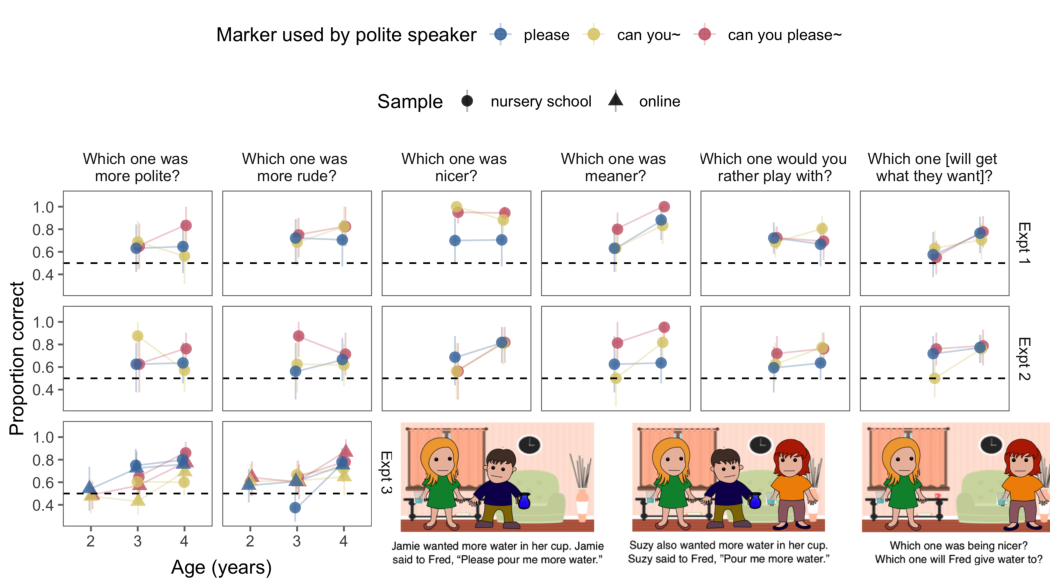
\includegraphics[width=0.9\linewidth]{erica_yoon_dissertation_files/figure-latex/figResultsPlacement-1} 

}

\caption[Speaker ratings for Experiments 2.1-2.3]{Bottom right: Story example. Top, left: Results. Proportion of correct responses to questions comparing between a speaker who used a politeness marker (where blue indicates "please", yellow "can you", and red "can you please") versus a speaker who did not. Data are binned into one-year age groups. Each row represents data from a different Experiment. Columns represent different questions asked. Dashed line represents chance level (i.e., if participant were guessing at random).}\label{fig:figResultsPlacement}
\end{figure*}
\elandscape

We looked at the proportion of correct responses to various questions
comparing speakers who used a politeness marker and spoke kindly, and
speakers who did not use a politeness marker and spoke meanly
(Figure~\ref{fig:figResultsPlacement}, first row). A mixed-effects
logistic regression predicting accuracy based on age, question type and
politeness marker type\footnote{for Experiments 1 and 2, we use this
  model structure with a maximal random effect structure that converges:
  \texttt{accuracy\ \textasciitilde{}\ age\ x\ question\ type\ x\ politeness\ marker\ type\ +\ (1\ \textbar{}\ item)},
  where age is continuous, centered and scaled. All categorical
  variables were deviation coded, with specified contrasts of interest
  for the question type. Significance was calculated using the standard
  normal approximation to the \(t\) distribution (Barr, Levy, Scheepers,
  \& Tily, 2013a).} showed there was an improvement with age (\(\beta\)
= 0.2, \(p =\) 0.026). The regression model also revealed that children
seemed to find some question types easier than others: Responses to
\emph{nice} and \emph{mean} questions were more accurate than to
\emph{polite} and \emph{rude} questions (\(\beta\) = 0.8, \(p =\)
0.002), whereas social implication questions (\emph{play partner} and
\emph{compliance}) were overall more difficult compared to speaker
attribute questions (\emph{polite}, \emph{rude}, \emph{nice}, and
\emph{mean}; \(\beta\) = -0.33, \(p =\) 0.006).

Looking more closely at responses for each of the question types,
children from both age groups tended to accurately answer the
\emph{polite}, \emph{nice}, \emph{mean}, \emph{rude}, and \emph{play
partner} questions overall (3-year-olds' mean accuracy range: 0.58 -
0.88; 4-year-olds' mean accuracy range: 0.68 - 0.9), indicating
correctly that the speaker who used a politeness marker was more polite
and nicer, and less mean and rude, and was likely a better play partner.
For the \emph{compliance} question, 4-year-olds overall answered
correctly that the speaker who used politeness marker will likely get
what they want from the listener (\(M_{4y}\) = 0.75, \(p\) \textless{}
.01), but 3-year-olds did not perform above chance (\(M_{3y}\) = 0.58).
As for the different politeness marker types, both age groups overall
tended to give correct answers based on all three markers, but
especially ``can you please'' (3-year-olds: \(M_{please}\) = 0.66,
\(M_{can you}\) = 0.72, \(M_{can you please}\) = 0.74; 4-year-olds:
\(M_{please}\) = 0.73, \(M_{can you}\) = 0.77, \(M_{can you please}\) =
0.84).

In sum, in this first experiment, we saw preliminary evidence that
children pay attention to some cues to politeness and are able to use
these cues to infer whether speakers are relatively polite, rude, nice
or mean, and whether speakers are good play partners and are likely to
get what they wanted from their addressees. 4-year-olds answered
questions accurately more often compared to 3-year-olds, especially for
the question about addressee's compliance with the speaker's request. In
general, however, both age groups tended to be accurate when all the
possible cues were used to signal that one speaker was polite (used
``can you please'', spoke with a kind tone and face) and the other
speaker wasn't (did not use a politeness marker, spoke with an angry
tone and face).

There were a number of remaining issues from Experiment 1. Children may
not have used the linguistic politeness markers (e.g., ``please'') per
se, and rather prosodic and facial cues that accompany these markers.
That is, children may have relied on the speaker's kind voice and face
rather than their use of ``please'' to evaluate their niceness or
likeability as a play partner. Similarly, greater accuracy for some
questions over others (e.g., \emph{nice} \textgreater{} \emph{polite})
may have been due to greater association between some of the words and
prosodic and facial cues (e.g., a kind face may be seen to signal
niceness more than politeness), not due to greater understanding for
those words or concepts. Another concern is that the experimenter was
aware of the manipulations (i.e., they knew which speaker was supposed
to be ``polite'') and thus could have affected the presentation of these
speakers in ways that are not consistent across all participants. In our
next two experiments, we sought to remove these potential confounds.

\section{Experiment 2}\label{experiment-2}

In Experiment 1, we saw initial evidence that children can use some
combinations of linguistic, prosodic, and facial cues to politeness. In
Experiment 2, we examined whether children can make similar judgments
using linguistic and prosodic cues only, without facial expressions. For
this, we conducted a preregistered experiment where we used pre-recorded
voiceovers to present speaker utterances, so that (1) we could look at
children's judgments based on linguistic markers and prosodic cues only,
and (2) we could remove the role of the experimenter in presentation of
these utterances.

\subsection[Methods]{\texorpdfstring{Methods\footnote{See pre-registered
  method, hypotheses and analysis plans at
  \url{https://osf.io/qkn8m/register/5771ca429ad5a1020de2872e}.}}{Methods}}\label{methods-1}

\subsubsection{Participants}\label{participants-1}

3-year-old (\(n=\) 16; 8 F, \(M_{age}\) = 3.56 years, \(SD_{age}\) =
0.29) and 4-year-old children (\(n=\) 22; 13 F, \(M_{age}\) = 4.5 years,
\(SD_{age}\) = 0.32) were recruited from a local preschool. An
additional 5 children were tested but excluded due to failure on the
practice questions.

\subsubsection{Stimuli and design}\label{stimuli-and-design-1}

The design was identical to Experiment 1. Stimuli were the same as
Experiment 1 except two changes: (1) Instead of a picture book, we
presented the stories on a tablet; (2) the speakers' utterances were now
presented as recorded voiceovers. The voiceovers were recorded by native
English speakers, and contained prosodic cues that matched the
presence/absence of a politeness marker (e.g., ``Please pour me more
water'' was recorded with a kind voice and ``pour me more water'' with
an angry voice).

\subsubsection{Procedure}\label{procedure-1}

The procedure was identical to Experiment 1, except for the following
change: The participants now had to tap on a speaker on tablet in order
either to hear them speak, or to choose an answer to the questions
asked.

\subsection{Results and Discussion}\label{results-and-discussion-1}

Overall we saw similar patterns of results in Experiment 2
(Figure~\ref{fig:figResultsPlacement}, second row) compared to Exp. 1. A
mixed-effects logistic regression predicting accuracy based on age,
question type and politeness marker type showed that accuracy improved
with age (\(\beta\) = 0.25, \(p =\) 0.002), and children made accurate
judgments more often when the politeness marker was ``can you please''
than when the marker was ``please'' or ``can you'' (\(\beta\) = 0.33,
\(p =\) 0.019). There was no main effect of question type, but there was
an interaction between age and question type such that performance for
\emph{nice} and \emph{mean} questions saw greater improvement with age
than for \emph{polite} and \emph{rude} questions (\(\beta\) = 0.57,
\(p =\) 0.011).

For children's responses to different question types, 3-year-olds'
accuracy did not differ from chance level for \emph{nice}, \emph{mean},
and \emph{play partner} questions, but their means numerically exceeded
50\% for all question types, and 4-year-olds accurately answered
questions of all types (3-year-olds' mean accuracy range: 0.6 - 0.88;
4-year-olds' mean accuracy range: 0.66 - 0.9). For politeness marker
types, 3-year-olds' performance did not differ from chance for
``please'' and ``can you'', but both age groups tended to answer
questions about different politeness markers accurately overall
(3-year-olds: \(M_{please}\) = 0.63, \(M_{can you}\) = 0.61,
\(M_{can you please}\) = 0.72; 4-year-olds: \(M_{please}\) = 0.7,
\(M_{can you}\) = 0.72, \(M_{can you please}\) = 0.8).

In sum, across Experiments 1 and 2, we saw that children tend to make
accurate judgments about speakers given their use of politeness markers,
especially ``can you please,'' together with prosodic cues, and children
get better with age in their use of politeness cues to respond to
questions about speaker attributes and social implications.

\section[Experiment 3]{\texorpdfstring{Experiment 3\footnote{See
  pre-registered method, hypotheses and analysis plans at
  \url{https://osf.io/rjsx5/register/5771ca429ad5a1020de2872e}.}}{Experiment 3}}\label{experiment-3}

We conducted a third, pre-registered experiment to see whether children
are able to evaluate speakers based on linguistic markers only, without
any other supporting cues such as prosodic cues or facial expressions.

\subsection{Methods}\label{methods-2}

\subsubsection{Participants}\label{participants-2}

We recruited two samples of participants: one from the same local
nursery school as Experiments 1 and 2, and the other from Lookit
(\url{https://lookit.mit.edu/}), an online platform for child research
participation, in which parents and their children can participate
together. The nursery school sample consisted of 3-year-old (\(n=\) 24;
11 F, \(M_{age}\) = 3.65 years, \(SD_{age}\) = 0.26) and 4-year-old
children (\(n=\) 25; 13 F, \(M_{age}\) = 4.48 years, \(SD_{age}\) =
0.28). An additional 3 children were tested but excluded due to failure
on the practice questions. The online sample consisted of 2-year-old
(\(n=\) 23; 12 F, \(M_{age}\) = 2.48 years, \(SD_{age}\) = 0.29),
3-year-old (\(n=\) 31; 15 F, \(M_{age}\) = 3.59 years, \(SD_{age}\) =
0.27) and 4-year-old children (\(n=\) 27; 12 F, \(M_{age}\) = 4.46
years, \(SD_{age}\) = 0.29). An additional 28 children were tested but
excluded due to failure on the practice questions (\(n=\) 19) or
completion of fewer than half of the test trials (\(n=\) 9).

\subsubsection{Stimuli}\label{stimuli}

For the nursery school sample, stimuli were identical to Experiment 2
except that the voiceovers for all utterances had the same prosody: All
utterances ended with a rising intonation. For the online sample,
stimuli were identical to what the nursery school participants saw
except that the story narrations (other than speaker utterances) were
also pre-recorded such that parents did not need to read the stories
aloud to their children.

\subsubsection{Procedure}\label{procedure-2}

For the nursery school sample, the procedure was identical to Experiment
2. For the online sample, the procedure was similar except that parents
and children participated together at home and there was no experimenter
present. Parents accessed the webpage for the study and gave their
consent for participation, and then read instructions to proceed through
the different stories, which specifically asked the parents to not tell
their children correct answers for the questions.

\subsection{Results and Discussion}\label{results-and-discussion-2}

\subsubsection{Experiment 3}\label{experiment-3-1}

For Experiment 3, we were able to look at how children answered the
\emph{polite} and \emph{rude} questions given the same three politeness
marker types as in Experiments 1 and 2, with three age groups including
2-year-olds. (Fig. ~\ref{fig:figResultsPlacement}, third row).

A mixed-effects logistic regression controlling for the effect of
sample\footnote{Model structure:
  \texttt{accuracy\ \textasciitilde{}\ sample\ +\ age\ *\ question\ type\ *\ politeness\ marker\ type\ +\ (1\ \textbar{}\ item)}}
showed improvement with age (\(\beta\) = 0.19, \(p =\) 0.033) as well as
better performance for ``can you please'' than ``please'' and ``can
you'' together (\(\beta\) = 0.42, \(p =\) 0.002), consistent with
Experiment 2 results. Performance for ``please'' was also better than
for ``can you please'' and ``please'' together (\(\beta\) = 0.3, \(p =\)
0.027), which may be surprising given that we previously did not see the
same effect in Experiments 1 and 2. One possible explanation is that
controlling for prosodic cues in Experiment 3 actually made it
\emph{easier} to use ``please'' as a politeness cue. Because we had
stripped all the other variations, it may have made the contrast between
the presence and absence of the marker ``please'' \emph{more} salient.

Additionally, children were better with the \emph{polite} questions than
\emph{rude} overall (\(\beta\) = -0.19, \(p =\) 0.04), but especially
given ``please'' (\(\beta\) = 0.42, \(p =\) 0.002). Finally, children
showed a greater improvement with age for ``can you please'' compared to
``please'' and ``can you'' together (\(\beta\) = 0.38, \(p =\) 0.004).

\subsubsection{All experiments}\label{all-experiments}

Did children perform better given facial and/or prosodic cues, or were
linguistic politeness markers sufficient? To see any potential effect of
experiment on children's performance, we conducted an exploratory
mixed-effects logistic regression on all three experiments
together\footnote{Model structure:
  \texttt{accuracy\ \textasciitilde{}\ sample\ +\ experiment\ +\ age\ *\ question\ type\ *\ politeness\ marker\ type\ +\ (1\ \textbar{}\ item)}}.
The regression model showed no significant main effect of experiment,
suggesting that children did not perform more poorly when facial and
prosodic cues were removed, and they were able to make accurate
judgments based on linguistic cues alone. The model also showed that
children improved with increasing age (\(\beta\) = 0.33, \(p\)
\textless{} .001) and that children were more accurate with ``can you
please'' than ``please'' and ``can you'' (\(\beta\) = 0.25, \(p =\)
0.011), confirming results from each individual experiment.
Additionally, the model showed that children became better at judging
the politeness marker ``can you please'' with age (\(\beta\) = 0.73,
\(p =\) 0.005), and that children answered \emph{polite} questions
better than \emph{rude} questions about the marker ``please'' (\(\beta\)
= 0.26, \(p =\) 0.006)

\section{General Discussion}\label{general-discussion}

What do young children understand about polite speech? In three
experiments, we looked at how 2- to 4-year-old children reason about
making requests with or without simple politeness markers such as
``please'', ``can you'' and ``can you please.'' By 3 years, children pay
attention to the use of politeness markers to accurately judge whether
that speaker is relatively more polite, rude, nicer or meaner compared
to another speaker. By 4 years, children reliably infer that a speaker
who uses a politeness marker is a better play partner and more likely to
get what they want. Across all three experiments, we saw a clear
developmental trend such that children improved in their reasoning about
polite speech with increasing age. We observed no large experiment
effects as we eliminated facial and prosodic cues; instead, all these
inferences appeared to be supported by linguistic markers alone.

Even though children have been shown to produce polite speech such as
``please,'' evidence has been sparse and inconclusive for whether young
children below 5 years comprehend speaker attributes and intentions
based on polite speech. Here, we found that children are sensitive to
the use of politeness markers in speech, and are able to use these
markers to infer the speaker's attributes (e.g., niceness) by 3 years,
and consequent social implications by 4 years. These ages are closer to
the age of first reliable production of polite speech than have been
suggested by earlier work.

Children in the US are often explicitly taught and prompted to use
politeness markers such as ``please'' in their requests from early on
(e.g., ``What's the magic word?''; Gleason et al., 1984), thus they may
quickly learn to use these markers as a rule in order to get what they
want. They also might hear other remarks that pair politeness markers
with positive words (e.g., ``You should be \emph{nice} and say
\emph{please}''), which may help them learn the association between
polite speech and positive attributes. Gradually, children may recognize
more subtle social processes that are related to polite speech
production: Adults may praise and reward children who spoke politely,
and children themselves may like peers who ask for permission to play
with their toys rather than take the toys away without asking. Future
work with corpus data analysis looking at these interactions between
children and others may reveal important conversational patterns that
help children acquire social meanings of polite speech.

There are limitations to the current work that present other
opportunities for future research. Because this work looked only at the
behaviors of English-speaking children with a relatively high
socioeconomic status in the US, it is an open question how children with
different language and cultural background may develop understanding of
polite speech. Cross-cultural investigation of what markers are present
in other languages, cultures and backgrounds, as well as how those
markers are acquired, will be informative.

Also, we did not manipulate the social status of speakers or addressees.
Though not explicitly stated, the visual depiction and narration used
for the current work suggested that speakers were communicating with
their peers only. However, one key prediction from politeness theory is
that speakers will adjust their utterances based on the status of the
addressees (P. Brown \& Levinson, 1987). Indeed children adjust own
their speech based on the listener status and age: Even at two years,
children use a polite form of request (``Can I have\ldots{}'') to an
adult but an imperative form (``Give me\ldots{}'') to a peer (Shatz \&
Gelman, 1973). Thus, future work should examine how children use cues to
politeness to judge speaker intentions in different contexts, including
varied status differences between speakers and listeners.

In sum, the current work showed that young children understand
implications of using simple politeness markers in requests. A broader
understanding of the emergence of politeness may offer insights into how
children become proficient users of language across the wide range of
social situations that they encounter.

\chapter{Children consider tradeoffs between informational and prosocial
goals to evaluate
speakers}\label{children-consider-tradeoffs-between-informational-and-prosocial-goals-to-evaluate-speakers}

\chaptermark{Children's understanding of goal tradeoffs}

In the last Chapter, I reported on empirical evidence that children are
sensitive to speakers' goals to be prosocial and kind. In this Chapter I
examine whether older children are capable of a more sophisticated
reasoning about the tradeoff between speakers' prosocial and
informational goals, using a case study of prosocial lies (versus blunt
truths). We show that adults and 5- to 8-year-old children reason about
goal tradeoffs based on context at hand, and understand that the same
lie (e.g., ``your cookie was tasty'') should be judged differently
depending on the speaker's goals, whether the speaker meant to be kind
or simply misleading without any apparent reason.

\section{Introduction}\label{introduction-2}

Imagine your friend bakes some cookies for you, but the cookies are hard
and salty and taste simply terrible. If your friend asks how you like
the cookies, must you admit, ``these cookies taste terrible,'' or is it
acceptable to say: ``They are delicious''? The latter is misleading but
gives the listener what she might want to hear----in other words, it
would be polite.

Politeness violates a critical principle of cooperative communication:
exchanging information efficiently and accurately (Grice, 1975). If
information transfer was the only currency in communication, a
cooperative speaker would find polite utterances undesirable because
they are potentially misleading. People are polite, however, and
speakers do produce polite utterances. Adults spontaneously produce
requests in polite forms (Clark \& Schunk, 1980), and exhibit politeness
strategies even while arguing, preventing unnecessary offense to their
interactants (T. Holtgraves, 1997). Listeners even attribute ambiguous
speech to a polite desire to hide a truth that could hurt another's
self-image (e.g. Bonnefon et al., 2009). In fact, it is difficult to
imagine human speech that efficiently conveys only the truth.
Intuitively, politeness is one prominent characteristic that
differentiates human speech from stereotyped robotic communication,
which may try to follow rules to say ``please'' or ``thank you'' yet
still lack genuine politeness.

Does this mean people are not cooperative communicators? P. Brown \&
Levinson (1987) recast the notion of a cooperative speaker as one who
has both an informational goal to improve the listener's knowledge state
as well as a prosocial goal to minimize any potential damage to the
hearer's (and the speaker's own) self-image, which they called
\emph{face.} In their analysis, if the speaker's intended meaning
contains no threat to the speaker or listener's face, then the speaker
will choose to convey the meaning in an efficient manner, putting it
\emph{on the record}. As the degree of face-threat becomes more severe,
however, a speaker will choose to be polite by producing more indirect
utterances.

One possible proposal based on this idea by P. Brown \& Levinson (1987)
is that people think about polite language as reflecting a tradeoff
between information transfer and face-saving. When you try to save face,
you hide or you risk losing some information in your intended message by
making your utterance false or indirect to some degree. When you
prioritize truthfulness and informativity, you may risk losing
listener's (or your own) face. In the current study, we examine whether
and how children and adults may think about polite speech this way: Do
they reason about polite speech as reflecting a tradeoff between the
goals of information transfer and face-saving?

From very early on, children seem to understand both informational and
social concerns behind language use. Around one year of age, children
already start to adjust their own informativeness in their communicative
action depending on the listener needs (Liszkowski, Carpenter, \&
Tomasello, 2008), and as they get older they correctly judge a speaker's
truthfulness and preferentially learn from informants who were
previously accurate (Corriveau, Meints, \& Harris, 2009). By 6 years
they are able to readily judge whether teachers are being
underinformative (Gweon, Pelton, Konopka, \& Schulz, 2014). Children
also understand speakers' goals to be kind, as 3- to 4-year-olds reason
that those who say ``please'' are nicer and more polite, and are likely
to be better play partners (Yoon \& Frank, 2019).

Even though previous research has suggested that children consider
informational and social goals that speakers have, it is unclear how
they might reason these goals together. For example, do children think
of the goals to be informative and to be kind as separate, fixed
\emph{rules} to follow, or do they make \emph{inferences} that accounts
for both goals that the speaker may consider? One possibility is that
children have a rule-based approach to language: They may think about
deterministic, separate rules such as ``If you want something, then you
should say \emph{please}'' and ``If you see/feel/think \emph{X}, then
you should (truthfully) say \emph{X.}'' Children can use these rules to
both produce polite and truthful utterances themselves, and evaluate
speakers based on whether they follow these rules or not (``She is nice
because she said \emph{please}''; or ``She is bad/wrong because she said
these cookies are tasty but they are actually salty and yucky.'')

While these rules can make language production and understanding easy
and straightforward, speakers often do not follow these rules
deterministically. For example, people sometimes tell the truth (``Those
herbs are poisonous, you shoudn't eat them'') but at other times they
tell lies to be kind (``This is a very delicious salad that you
prepared!''). Indeed, caregivers contradict their own teachings as they
demand children to tell the truth in some contexts (``Who broke the
vase? Be honest.''), but reproach them for telling the truth in other
contexts (Child: ``This {[}meal that Grandma cooked{]} is yucky''
Father:``Don't say that, you should be nice!''). Thus, language users
ultimately need to learn that language reflects not only simple
deterministic rules to follow, but also more nuanced tradeoffs between
different goals that speakers might have depending on the situation.

Do adults and children go beyond simple rules and engage in an
\emph{inference}-based reasoning to think about how speech reflects goal
tradeoffs? Here we look at a case study of prosocial lies (versus blunt
truths) to examine whether children understand the tradeoff between
speakers' informational goals and prosocial goals. For example, if Alice
asked Bob for feedback on her performance that was poor in quality
(e.g., cookies she baked that were salty or a presentation she gave that
was unintelligible), Bob would be in a bind: On one hand, he would want
to be informative and convey accurate information, which would lead him
to say ``{[}Your cookies{]} were terrible.'' On the other hand, he would
also want to be prosocial and kind, and make Alice feel happy and
respected, by saying ``{[}Your cookies{]} were delicious.'' In such
context, telling a lie would indicate that the speaker chose to
prioritize the goal to be kind, whereas telling the truth would indicate
the speaker's priority for the goal to be informative. Critically,
however, Bob should have a good reason to lie; if Alice was asking about
some cookies Bob himself got from a store instead of cookies that she
baked, then Bob would have no reason to lie to Alice and say that the
cookies were ``delicious,'' which would only be misleading. Thus, in
order to reason about speaker intentions and goal tradeoff
considerations correctly, people need to account for the context in
which the utterance was produced.

Previous research suggests that children \emph{produce} prosocial lies
(utterances that are dishonest yet kind) appropriately depending on
context from early on. There is evidence that by 3 years, children start
to tell white lies, and e.g., say that an adult ``looks okay for the
picture'' even though she has a conspicuous mark of lipstick on her nose
(Talwar \& Lee, 2002), or lie to a gift-giver about her gift that they
actually found undesirable (Talwar et al., 2007).

But do children \emph{understand} that prosocial lies reflect speakers'
priority to be prosocial over being truthful and informative? Children
do seem to be sensitive to speakers' prosocial intentions: By 4 years,
children evaluate lies differently depending on whether the lies were
told to be kind to the listener (e.g., ``Your new hat looks great'') or
to hide their own misdeed {[}``Yes, I brushed my teeth''{]}, judging the
latter to be worse (Bussey, 1999). 7- to 11-year-old children also tend
to rate lie-telling more favorably in politeness situations (e.g.~a
teacher gave the protagonist an undesirable gift) than in transgression
situations (e.g.~the protagonist damaged a library book; G. D. Heyman et
al., 2009).

It is an open question, however, whether children evaluate the exact
same lie differently depending on the perceived goal tradeoff. For
example, saying ``your cookies were tasty'' may be an acceptable lie if
the listener baked those cookies as a gift for the speaker, but the same
lie might only be misleading and not helpful if the listener did not
bake the cookies himself but simply wanted to taste the cookies.
Likewise, telling the truth ``the cookies were yucky'' may seem blunt
and harsh if the speaker is talking to the person who baked the cookies,
but the same utterance can be reasonable and even helpful if the
listener simply wants to taste the cookies and is curious how the
speaker liked them. In the current study, we ask whether children are
able to reason about polite liars versus blunt truth-tellers, on the
dimensions of information transfer (being honest) vs.~face-saving (being
nice/mean).

\section{Method}\label{method}
\begin{table}[t]

\caption[Participant demographic information for Chapter 3.]{\label{tab:childInfSample}Participant demographic information.}
\centering
\resizebox{\linewidth}{!}{
\begin{tabular}{lllll>{\raggedright\arraybackslash}p{2.2cm}>{\raggedright\arraybackslash}p{2.2cm}}
\toprule
\textbf{Sample} & \textbf{Condition} & \textbf{Age group} & \textbf{Total N} & \textbf{Female} & \textbf{Mean age (years)} & \textbf{SD age (years)}\\
\midrule
original & Control (no reason for dishonesty) & 5-6-yr & 26 & 16 & 5.92 & 0.45\\
original & Control (no reason for dishonesty) & 7-8-yr & 19 & 11 & 7.94 & 0.59\\
original & Control (no reason for dishonesty) & adult & 76 &  &  & \\
original & Experimental (politeness reasons) & 5-6-yr & 24 & 14 & 5.99 & 0.69\\
original & Experimental (politeness reasons) & 7-8-yr & 18 & 7 & 8.08 & 0.69\\
\addlinespace
original & Experimental (politeness reasons) & adult & 71 &  &  & \\
replication & Both control and experimental & 5-6-yr & 33 & 21 & 5.98 & 0.58\\
replication & Both control and experimental & 7-8-yr & 31 & 15 & 7.91 & 0.56\\
\bottomrule
\end{tabular}}
\end{table}
\subsection{Participants}\label{participants-3}

We recruited parents and their children at Children's Discovery Museum
of San Jose, and adults through Amazon's Mechanical Turk. We recruited
two samples: a first, \emph{original} sample and a second,
pre-registered \emph{replication} sample\footnote{see
  \url{https://osf.io/u4v7y/register/5771ca429ad5a1020de2872e} for
  pre-registered method, hypotheses and analysis plans.}. Participant
demographic information is shown in Table~\ref{tab:childInfSample}.

As part of the task, we included training trials where children and
adults were tested on the meanings of important keywords such as
``nice'', ``mean'', and ``truth.'' For example, participants were asked:
``Nicole gave her friend a gift. Was Nicole nice? Was Nicole mean?'' We
excluded participants who gave wrong answers on these trials, which led
to exclusion of 2 child participants from the original sample.

\subsection{Stimuli and design}\label{stimuli-and-design-2}

We presented stories in which some characters (\emph{speakers}) were
asked to give evaluative feedback on something bad that they just
experienced (e.g., a yucky cookie that they tasted, or a boring game
that they played). There were two different \emph{context} conditions:
In the \emph{experimental} condition, speakers were asked by listeners
to comment on something that the listeners themselves had created, which
provides the speakers with politeness reasons to lie and hide the poor
quality of the product in order to not hurt the listener's feelings. For
example, one story in the experimental condition read: ``Look, this is
Edward {[}the listener{]}! One day, Edward decided to bake some cookies.
Edward brought his cookie to school and met his friend Mary {[}the
speaker{]}. Edward said to his friend Mary, ``Here, try my cookie!''
Mary tasted the cookie, and she did not like the cookie at all --- she
thought the cookie tasted yucky! Edward asked Mary, ``Mary, how did you
like my cookie?'' Mary told Edward, ``Edward, your cookie was
tasty.''\,'' In the \emph{control} context condition, speakers were
asked by listeners to comment on something that they stumbled upon, not
what the listeners created (and thus had no reasons to lie about the
quality of the product). The cookie story in the control condition read:
``Look, this is Mary! One day, Mary saw a free cookie. Mary said, ``It's
a free cookie, I'll try it!'' Mary tasted the cookie, and she did not
like the cookie at all --- she thought the cookie tasted yucky! Mary's
friend Edward also wanted to taste the cookie. Edward asked Mary,
``Mary, how did you like the cookie?'' Mary told Edward, ``Edward, the
cookie was tasty.''\,'' For the original sample, each participant saw
only one of the two conditions (i.e., context was a between-participants
variable), whereas for the replication sample, each participant saw both
conditions (within-participants).

Each story presented two episodes that each presented a different
\emph{speaker type}: one who told a lie and the other who told the
truth. After presenting what each speaker decided to say, we presented
three \emph{question types}, asking participants to judge (1) whether
the speaker told the truth; (2) whether the speaker was nice; and (3)
whether the speaker was mean. For the original sample, each participant
heard two stories from the same condition (either experimental or
control); for the replication sample, each participant heard four
stories, two from each condition.

After presenting the two episodes, we asked participants to compare the
two speakers and select a better play partner (``Who do you want to play
with more, Sally or Mary?'') and the reason for their answer. The order
of context conditions, speaker types and question types was
counterbalanced across participants. Training trials and full example
stories are provided in Supplementary Materials.

\subsection{Procedure}\label{procedure-3}

For child participants, the experimenter read the storybook with
children in a room in a children's museum. They were first introduced to
the storybook with simple stories to familiarize them with keywords like
``nice,'' ``mean,'' and ``truth'' (e.g., ``Pam ate five cookies, but Pam
told her mom a lie that she didn't eat any cookie. Was Pam telling the
truth?''). Then the experimenter read two (original) or four
(replication) stories to each participant. While reading each episode,
experimenters checked for the participants' comprehension twice by
asking whether the speaker liked the product (e.g., ``So did Sally like
the cookie or did she not like the cookie?'') and what the speaker told
the listener (``So what did Sally tell Edward again?''). If the
participant gave an incorrect answer to these comprehension check
questions, the experimenter said ``let's think about that one more
time,'' and repeated the story. For adult participants, we presented the
same stories that children heard in an online task (see
\url{http://langcog.stanford.edu/expts/EJY/trupol/adult/trupol.html} for
the online task that adults completed).

\section{Results and Discussion}\label{results-and-discussion-3}

\subsection{Speaker ratings: truth-telling, niceness,
meanness}\label{speaker-ratings-truth-telling-niceness-meanness}
\begin{figure*}[p]

{\centering 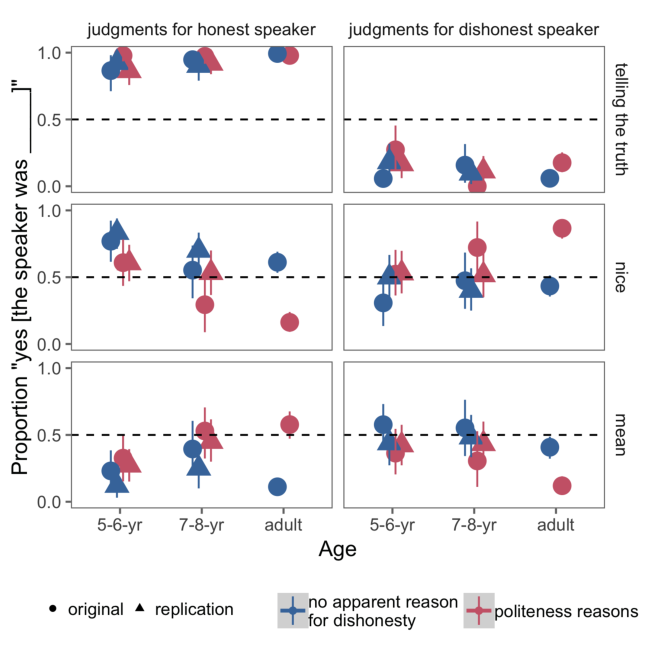
\includegraphics[width=0.9\linewidth]{erica_yoon_dissertation_files/figure-latex/figTrupolResultsPlacement-1} 

}

\caption[Speaker ratings for the experiment in Chapter 3.]{Speaker ratings by different age groups (x-axis) for the honest speaker (left column) and the dishonest speaker (right), in different contexts (colors). Rows represent question types (e.g., Was Sally telling the truth?), and y-axis represents proportion saying ``yes" to the question. Shapes represent original (circles) vs. replication samples (triangles). }\label{fig:figTrupolResultsPlacement}
\end{figure*}
\begin{table}[tbp]
\begin{center}
\begin{threeparttable}
\caption{\label{tab:trupol_brm}Predictor mean estimates with standard deviation and 95\% credible interval information for a Bayesian linear mixed-effects model predicting ''yes" responses to questions.}
\begin{tabular}{lllll}
\toprule
Predictor & \multicolumn{1}{c}{Mean} & \multicolumn{1}{c}{SD} & \multicolumn{1}{c}{95\% CI-Lower} & \multicolumn{1}{c}{95\% CI-Upper}\\
\midrule
Intercept & 3.20 & 2.72 & -2.91 & 9.35\\
Experimental condition (Expt) & 0.02 & 2.93 & -5.95 & 6.42\\
Niceness question (Nice) & -1.46 & 4.11 & -9.39 & 6.58\\
Meanness question (Mean) & -5.38 & 3.81 & -13.50 & 3.28\\
Dishonest speaker (Dishonest) & -5.94 & 3.39 & -12.78 & 1.87\\
Age & 0.29 & 0.32 & -0.31 & 0.96\\
Expt * Nice & -1.44 & 0.51 & -2.46 & -0.44\\
Expt * Mean & 1.37 & 0.55 & 0.30 & 2.42\\
Expt * Dishonest & -0.31 & 0.60 & -1.49 & 0.89\\
Nice * Dishonest & 3.89 & 0.62 & 2.72 & 5.15\\
Mean * Dishonest & 8.15 & 0.62 & 6.98 & 9.43\\
Expt * Age & 0.47 & 0.44 & -0.39 & 1.32\\
Nice * Age & -1.11 & 0.38 & -1.88 & -0.37\\
Mean * Age & 0.65 & 0.45 & -0.24 & 1.52\\
Dishonest * Age & -0.86 & 0.43 & -1.73 & -0.07\\
Expt * Nice * Dishonest & 2.34 & 0.69 & 0.98 & 3.70\\
Expt * Mean * Dishonest & -1.44 & 0.71 & -2.82 & -0.04\\
Expt * Nice * Age & -0.04 & 0.51 & -1.05 & 0.96\\
Expt * Mean * Age & -0.84 & 0.54 & -1.90 & 0.24\\
Expt * Dishonest * Age & -1.25 & 0.61 & -2.44 & -0.05\\
Nice * Dishonest * Age & 1.60 & 0.50 & 0.67 & 2.63\\
Mean * Dishonest * Age & 0.08 & 0.51 & -0.90 & 1.11\\
Expt * Nice * Dishonest * Age & 0.99 & 0.71 & -0.42 & 2.37\\
Expt * Mean * Dishonest * Age & 1.33 & 0.72 & -0.07 & 2.76\\
\bottomrule
\end{tabular}
\end{threeparttable}
\end{center}
\end{table}
The results from child and adult participants are plotted in
Figure~\ref{fig:figTrupolResultsPlacement}. We can make a few
qualitative observations for each of the question types: For the
truth-telling rating, adult and child participants correctly judged that
the honest speaker was indeed telling the truth, and that the dishonest
speaker was not telling the truth, regardless of the condition (top row
of Figure~\ref{fig:figTrupolResultsPlacement}). The niceness rating
varied by condition: Given politeness reasons, participants tended to
say that the dishonest speaker was nice more often and honest speaker
was nice less often (middle row of
Figure~\ref{fig:figTrupolResultsPlacement}). The meanness rating showed
the opposite pattern (bottom row of
Figure~\ref{fig:figTrupolResultsPlacement}).

Additionally, we also see a developmental trend. Adults showed the
clearest discrepancies in speaker ratings by condition and tended to be
much more charitable toward the dishonest speaker given politeness
reasons compared to no apparent reasons to lie. Older children
(7-8-year-olds) show similar patterns but with smaller rating
differences between the two conditions. Younger children (5-6-year-olds)
also differentiated between the two conditions but not as much as older
children and adults did, and younger children generally tended to rate
the honest speaker more favorably than the dishonest speaker across both
conditions.

We conducted statistical analysis to verify these qualitative
observations. We used a Bayesian linear mixed-effects model
(\texttt{brms} package in R; B��rkner, 2017) using crossed random
effects of participant, item and sample with the maximal random effect
structure supported by the design (Barr, Levy, Scheepers, \& Tily,
2013b; A. Gelman \& Hill, 2006). We ran the statistical model on the
child dataset only. Age is plotted in bins in
Figure~\ref{fig:figTrupolResultsPlacement}, but was analyzed as a
continuous variable, scaled and centered, in our statistical model.

The Bayesian linear mixed model\footnote{This model incorporated a few
  changes from the pre-registered model structure: whereas we
  pre-registered
  \texttt{brm(niceness rating $\sim$ age * condition * speaker + (speaker * condition | subject) + (speaker * condition | item)},
  we ran a more appropriate and inclusive model that contained question
  type as a main effect and a random effect of item, and corrected
  crossed random effects structure:
  \texttt{brm(answer ~ $\sim$ * condition * speaker type  * question type + (question type + speaker type | participant) + (condition + question type + speaker type | item) + (condition + question type + speaker type | sample)}..}
predicting ``yes'' responses based on participant age, context type
(control vs.~experimental), speaker type (honest vs.~dishonest) and
question type (truth-telling vs.~niceness vs.~meanness) showed a
positive interaction between experimental condition, dishonest speaker
and niceness judgment: Participants judged a dishonest speaker as nicer
in the experimental condition, where the speaker had politeness reasons
to lie to the listener, compared to the control condition where the
speaker had no apparent reasons to lie. Thus, children were indeed able
to evaluate the dishonest speaker's intentions differently based on the
context. There also was a positive interaction between dishonest speaker
and meanness rating, which indicates that a dishonest speaker was rated
as mean more often compared to the honest speaker overall regardless of
the condition.
\begin{figure*}[t]

{\centering 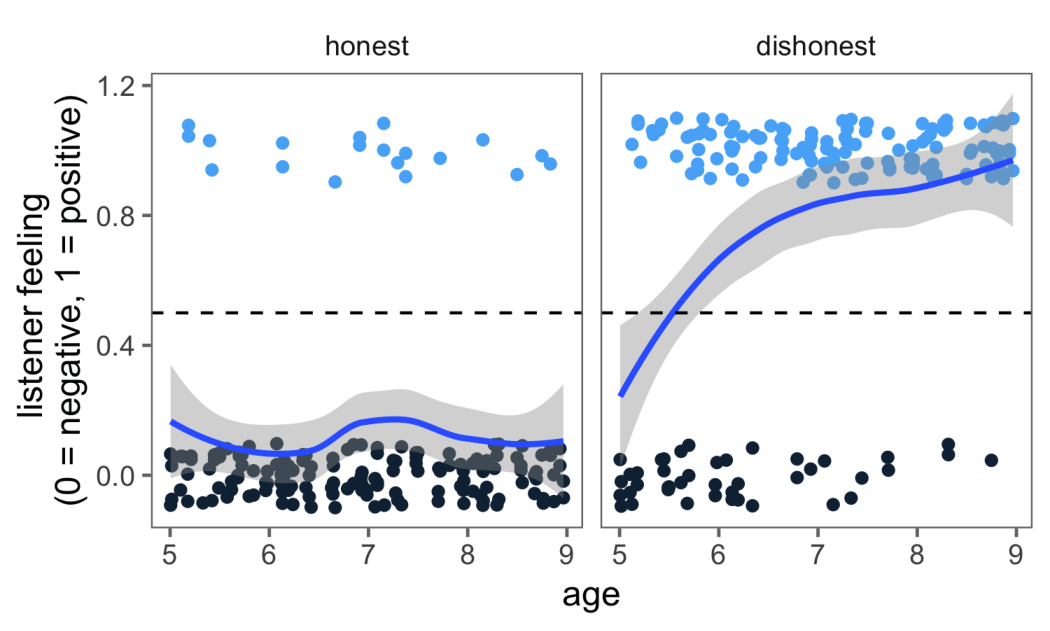
\includegraphics[width=0.9\linewidth]{erica_yoon_dissertation_files/figure-latex/figTrupolLfeelResultsPlacement-1} 

}

\caption[Listener feeling judgments in the experiment in Chapter 3.]{Children's judgments for listener feelings (y-axis) upon hearing the utterance of the honest versus dishonest speaker (columns), across age (x-axis).}\label{fig:figTrupolLfeelResultsPlacement}
\end{figure*}
Finally, there was also a positive interaction between participant age,
dishonest speaker and niceness judgment, which confirmed that children
judged the dishonest speaker as nice more often with increasing age, a
trend that extended to adulthood
(Figure~\ref{fig:figTrupolResultsPlacement}). Why did adults and older
children judge the dishonest speaker more favorably compared to younger
children? One possible explanation is older children are more proficient
at inferring other people's mental states (Wellman \& Liu, 2004),
leading them to place more weight on the addressee's feelings in
evaluating a white lie or blunt truth. Indeed, when asked about how the
listener would have felt upon hearing the polite liar's utterance, older
children tended to answer that the listener would have felt ``happy'',
``good'', or ``nice'' more often than younger children
(Figure~\ref{fig:figTrupolLfeelResultsPlacement}). Another possibility
is that younger and older children use different communicative goals;
younger children prioritize honesty, whereas older children value
politeness more. Finally, it is also possible that children's construal
of linguistic terms ``niceness'' and ``meanness'' may differ from adults
(see more detailed explanation in section ``Play partner selection''
below).

\subsection{Play partner selection}\label{play-partner-selection}
\begin{figure*}[t]

{\centering 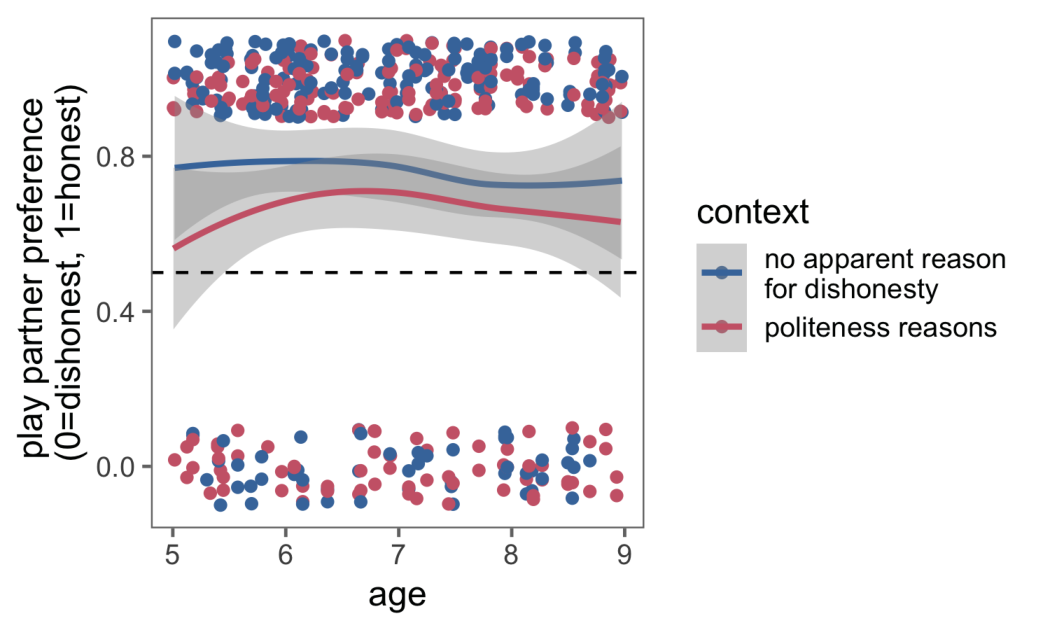
\includegraphics[width=0.9\linewidth]{erica_yoon_dissertation_files/figure-latex/figTrupolPlayPlacement-1} 

}

\caption[Play partner selection in the experiment in Chapter 3.]{Children's play partner selection between the honest speaker (1 on the y-axis) and dishonest speaker (0 on the y-axis) across age (x-axis), across the two context conditions (columns).}\label{fig:figTrupolPlayPlacement}
\end{figure*}
\begin{figure*}[t]

{\centering 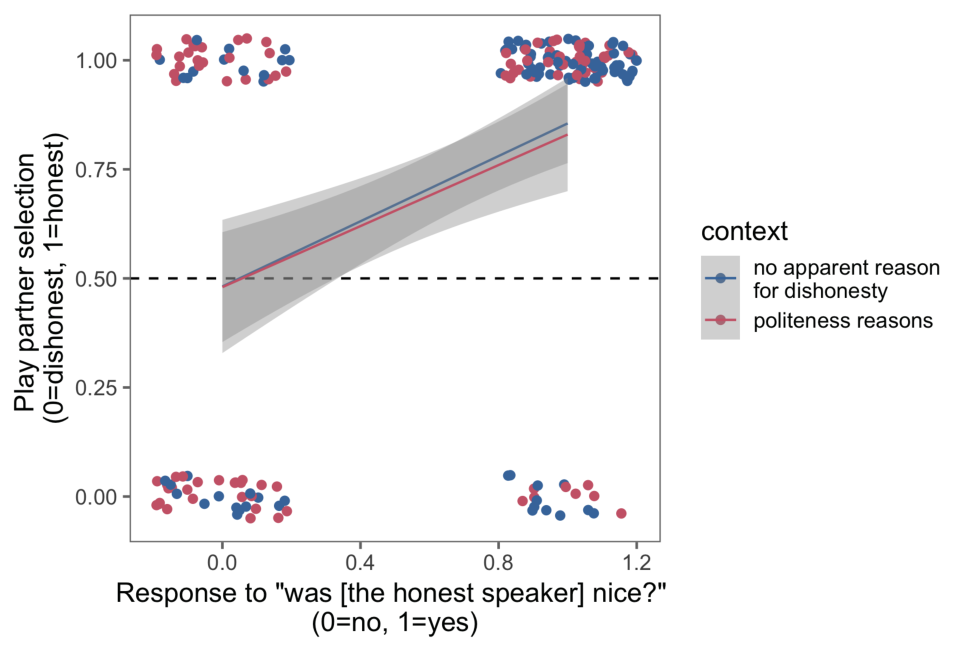
\includegraphics[width=0.9\linewidth]{erica_yoon_dissertation_files/figure-latex/figTrupolPlayNicePlacement-1} 

}

\caption[Play partner selection versus niceness judgment for the honest speaker in the experiment in Chapter 3.]{Children's play partner selection (y-axis) versus their nicess judgment for the honest speaker (x-axis) across age (x-axis), across the two context conditions (columns).}\label{fig:figTrupolPlayNicePlacement}
\end{figure*}
When asked to choose the speaker they would like to play with more,
children's preference for the honest speaker was slightly higher in the
control condition (i.e., given no apparent reason for dishonesty),
though in both conditions children selected the honest speaker as their
play partner more often overall
(Figure~\ref{fig:figTrupolPlayPlacement}). Children's play partner
choice differed depending on their niceness rating of the honest speaker
within the same trial (Figure~\ref{fig:figTrupolPlayNicePlacement}):
those who rated the honest speaker as ``nice'' were more likely to
prefer to play with the honest speaker, whereas those who rated the
honest speaker as ``not nice'' were divided between selecting the honest
speaker and dishonest speaker as their play partner.

Why did some children prefer to play with the honest speaker, even when
they rated the honest speaker as ``not nice'' given politeness reasons
to lie? Perhaps the niceness ratings and play partner preference have
different implications: Play partner choice could reveal the
participant's holistic judgment of the two speakers' personalities (``I
like Sally better because she tells the truth''), whereas judgment of
whether a given speaker is ``nice'' can depend on several factors, such
as the participant's evaluation of the speaker's personality (``Sally is
not a nice person''), the speaker's intention (``Sally was not trying to
be nice and instead wanted to tell the blunt truth'') and the construal
of the linguistic term ``nice'' (``Sally was not nice, because nice
means saying something positive like the cookie is tasty'').

\section{Conclusion}\label{conclusion}

In this work, we showed that both adults and 5- to 8-year-old children
were able to use context information to evaluate speaker intentions and
rate their niceness and meanness accordingly. This suggests that they
are sensitive to the tradeoffs between informational goals (pushing
toward truthfulness) and prosocial goals (pushing toward face-saving)
and reason about what goals should be prioritized depending on the
context.

There was also a trend for developmental differences in attribution of
niceness and meanness to prosocial liars versus blunt truth-tellers:
Younger children (5-6-year-olds) were more charitable toward blunt
truth-tellers in their rating of speaker niceness. However, it is still
an open question why younger and older children different in their
evaluation of the speaker intentions. Possibilities are (1) younger
children might prioritize the social concerns over informational
concerns compared to older children and adults; (2) their lack of
Theory-of-Mind abilities prevent them from understanding needs for
polite lies; or (3) their construal of linguistic terms like ``nice''
may differ from that of older children, and depend more on
rule-following and less on face-saving. Future work should tease apart
these possibilities by testing a broader set of utterances that reflect
more gradient tradeoff decisions between informational and social goals.
For example, the speaker could say ``I don't think this cookie is very
tasty'' to be somewhat informative but also somewhat face-saving at the
same time.

In sum, this work presented evidence that by 6 years children are able
to evaluate speakers differently based on context that affects tradeoff
of informational and social goals, though the ability to evaluate this
tradeoff may develop until adulthood.

\chapter[Adults consider tradeoffs between competing social goals to
predict polite language use]{\texorpdfstring{Adults consider tradeoffs
between competing social goals to predict polite language use\footnote{This
  chapter is submitted and currently under review at \emph{Open Mind},
  and is joint work with Michael Henry Tessler, Noah D. Goodman and
  Michael C. Frank.}}{Adults consider tradeoffs between competing social goals to predict polite language use}}\label{adults-consider-tradeoffs-between-competing-social-goals-to-predict-polite-language-use}

\chaptermark{Modeling polite speech}

Language is a remarkably efficient tool for transmitting information.
Yet human speakers make statements that are inefficient, imprecise, or
even contrary to their own beliefs, all in the service of being polite.
What rational machinery underlies polite language use? In this Chapter,
we present evidence that adults think of polite speech as emerging from
competing communicative goals: to convey information, to be kind, and to
present oneself in a good light. We formalized this goal tradeoff using
a probabilistic model of utterance production, which predicts human
utterance choices in socially-sensitive situations with high
quantitative accuracy, and we show that our full model is superior to
its variants with subsets of the three goals.

\section{Introduction}\label{introduction-3}

We rarely say exactly what's on our mind. Although ``close the window!''
could be an effective message, we dawdle by adding ``can you
please\ldots{}?'' or ``would you mind\ldots{}?'' Rather than tell an
uncomfortable truth, socially-aware speakers lie (``Your dress looks
great!'') and prevaricate (``Your poem was so appropriate to the
occasion''). Such language use is puzzling for classical views of
language as information transfer (Bühler, 1934; Frank \& Goodman, 2012;
Jakobson, 1960; Shannon, 1948). On the classical view, transfer ought to
be efficient and accurate: Speakers are expected to choose succinct
utterances to convey their beliefs (Grice, 1975; Searle, 1975), and the
information conveyed is ideally truthful to the extent of a speaker's
knowledge. Polite speech violates these basic expectations about the
nature of communication: It is typically inefficient and
underinformative, and sometimes even outright false. Yet even young
speakers spontaneously produce requests in polite forms (Axia \& Baroni,
1985), and adults use politeness strategies while arguing (T.
Holtgraves, 1997), even though polite utterances may risk high-stakes
misunderstandings (Bonnefon, Feeney, \& De Neys, 2011).

If politeness only gets in the way of effective information transfer,
why be polite? Clearly, there are social concerns, and most linguistic
theories assume utterance choices are motivated by these concerns,
couched as either polite maxims (Leech, 1983), social norms (Ide, 1989),
or aspects of a speaker and/or listener's identity, known as \emph{face}
(P. Brown \& Levinson, 1987; Goffman, 1967). Face-based theories predict
that when a speaker's intended meaning contains a threat to the
listener's face or self-image (and potentially the speaker's face), her
messages will be less direct, less efficient, and possibly untruthful.
Indeed, listeners readily assume speakers' intentions to be polite when
interpreting utterances in face-threatening situations (Bonnefon et al.,
2009). How this socially-aware calculation unfolds, however, is not well
understood. When should a speaker decide to say something false (``Your
poem was great!'' based on an example from Bonnefon et al. (2009))
rather than just be indirect
(\emph{Some of the metaphors were tricky to understand.})? How does a
speaker's own self-image enter into the calculation?

We propose a utility-theoretic solution to the problem of polite
language use by quantifying the tradeoff between competing communicative
goals. In our model, speakers attempt to maximize utilities that
represent their communicative goals: informational utility---derived via
classical, effective information transmission; social utility---derived
by being kind and saving the listener's face; and self-presentational
utility---the most novel component of our model, derived by appearing in
a particular way to save the speaker's own face. Speakers then produce
an utterance on the basis of its expected utility (including their cost
to speak). The lie that a poem was great provides social utility by
making the writer feel good, but does not provide information about the
true state of the world. Further, if the writer suspects that the poem
was in fact terrible, the speaker runs the risk of being seen as
uncooperative.

We assume that speakers' utilities are weighed within a probabilistic
model of pragmatic reasoning: the Rational Speech Act (RSA) framework
(Frank \& Goodman, 2012; N. D. Goodman \& Frank, 2016). Speakers are
modeled as agents who choose utterances by reasoning about their
potential effects on a listener, while listeners infer the meaning of an
utterance by reasoning about speakers and what goals could have led them
to produce their utterances. This class of models has been effective in
understanding a wide variety of complex linguistic behaviors, including
vagueness (Lassiter \& Goodman, 2017), hyperbole (Kao, Wu, Bergen, \&
Goodman, 2014), and irony (Kao \& Goodman, 2015), among others. In this
framework, language use builds on the idea that human social cognition
can be approximated via reasoning about others as rational agents who
act to maximize their subjective utility (Baker, Saxe, \& Tenenbaum,
2009), a hypothesis which has found support in a wide variety of work
with both adults and children (e.g., Jara-Ettinger, Gweon, Schulz, \&
Tenenbaum, 2016; S. Liu, Ullman, Tenenbaum, \& Spelke, 2017).
\begin{figure}[!t]

{\centering 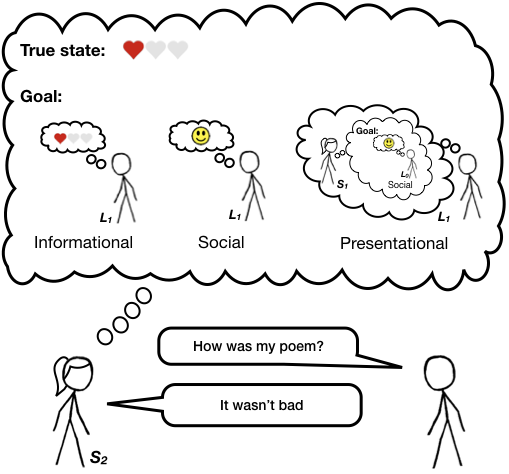
\includegraphics[width=0.9\linewidth]{/Users/ejyoon/Documents/Documents/Research/dissertation/index/chapter_child_rmds/ch4_modeling_polite/files/model} 

}

\caption[Graphical representation of the computational model of polite speech production and understanding.]{Diagram of the model: The polite speaker observes the true state and determines her goal between three utilities (informational, social, and presentational), and produces an utterance.}\label{fig:model}
\end{figure}
RSA models are defined recursively such that speakers \(S\) reason about
listeners \(L\), and vice versa. We use a standard convention in
indexing and say a pragmatic listener \(L_1\) reasons about what
intended meaning and goals would have led a speaker \(S_1\) to produce a
particular utterance. Then \(S_1\) reasons about a \emph{literal
listener} \(L_0\), who is modeled as attending only to the literal
meanings of words (rather than their pragmatic implications), and hence
grounds the recursion. The target of our current work is a model of a
polite speaker \(S_2\) who reasons about what to say to \(L_1\) by
considering informational, social, and self-presentational goals
(Figure~\ref{fig:model}).

We evaluate our model's ability to predict human utterance choices in
situations where polite language use is expected. Imagine Bob recited a
poem and asked Ann how good it was. Ann (\(S_2\)) produces an utterance
\(w\) based on the true state of the world \(s\) (i.e., the rating, in
her mind, truly deserved by Bob's poem) and a set of goal weights
\(\hat{\phi}\), that determines how much Ann prioritizes each of the
three possible goals. Ann's production decision is softmax, which
interpolates between maximizing and probability matching (via
\(\lambda_{S_2}\); N. D. Goodman \& Stuhlmüller, 2013):

\[P_{S_2}(w | s, \hat{\phi}) \propto \exp(\lambda_{S_2} \cdot \mathop{\mathbb{E}}[U_{total}(w; s; \hat{\phi}; \phi_{S_1})]).\]

We posit that a speaker's utility contains three distinct components:
informational, social, and presentational. The total utility
\(U_{total}\) of an utterance is thus the weighted combination of the
three utilities minus the utterance cost \(C(w)\):

\[U_{total}(w; s; \hat{\phi}; \phi_{S_1}) = \phi_{inf} \cdot U_{inf}(w; s) + \phi_{soc} \cdot U_{soc}(w) + \phi_{pres} \cdot U_{pres}(w; \phi_{S_1}) - C(w).\]

We define \emph{social utility} (\(U_{soc}\)) as the expected subjective
utility of the state \(V(s)\) implied to the pragmatic listener by the
utterance: \(U_{soc}(w) = \mathbb{E}_{P_{L_1}(s \mid w)}[V(s)]\). The
subjective utility function \(V(s)\) could vary by culture and context;
we test our model when states are explicit ratings (e.g., on a 4-point
scale) and we assume a positive linear value relationship between states
and values \(V\) to model a listener's preference to be in a highly
rated state (e.g., Bob would prefer to have written a poem deserving 4
points rather than 1 point).

At the same time, a speaker may desire to be epistemically helpful,
modeled as standard \emph{informational utility} (\(U_{inf}\)). The
informational utility indexes the utterance's \emph{surprisal}, or
amount of information the listener (\(L_1\)) would still not know about
the state of the world \(s\) after hearing the speaker's utterance \(w\)
(e.g., how likely is Bob to guess Ann's actual opinion of the poem):
\(U_{inf}(w) = \ln(P_{L_1}(s | w))\). Speakers who optimize for
informational utility produce accurate and informative utterances while
those who optimize for social utility produce utterances that make the
listener feel good.

If a listener is uncertain how their particular speaker is weighing the
competing goals to be honest vs.~kind (informational vs.~social
utilities), he might try to infer the weighting (e.g., ``was she just
being nice?''). But a sophisticated speaker can produce utterances in
order to appear \emph{as if} she had certain goals in mind, for example
making the listener think that the speaker was being both kind and
informative (``she wanted me to know the truth but without hurting my
feelings''). The extent to which the speaker \emph{appears} to the
listener to have a particular goal in mind (e.g., to be kind) is the
utterance's \emph{presentational utility} (\(U_{pres}\)). The speaker
gains presentational utility when her listener believes she has
particular goals, represented by a mixture weighting \(\phi_{S_1}\)
between trying to be genuinely informative vs.~kind. Formally,

\[U_{pres}(w; \phi_{S_1}) = \ln(P_{L_1}(\phi_{S_1} \mid w)) = \ln \int_s P_{L_1}(s, \phi_{S_1} \mid w).\]

\noindent The speaker conveys a particular weighting of informational
vs.~social goals (\(\phi_{S_1}\)) by considering the beliefs of listener
\(L_1\), who hears an utterance and jointly infers the speaker's
utilities and the true state of the world:

\[P_{L_1}(s, \phi_{S_1} | w) \propto P_{S_1}(w | s, \phi_{S_1}) \cdot P(s) \cdot P(\phi_{S_1}).\]

\noindent The presentational utility is the highest-order term of the
model, defined only for a speaker thinking about a listener who
evaluates a speaker (i.e., defined for \(S_2\), but not \(S_1\)). Only
the social and informational utilities are defined for the \(S_1\)
speaker (via reasoning about \(L_0\)); thus, \(S_1\)'s utility
weightings can be represented by a single number, the mixture parameter
\(\phi_{S_1}\). Definitions for \(S_1\) and \(L_0\) otherwise mirror
those of \(S_2\) and \(L_1\) and can be found in the Supplmentary
Materials: Model details section.

Finally, more complex utterances incur a greater cost, \(C(w)\) --
capturing the general pressure towards economy in speech. In our work,
utterances with negation (e.g., \emph{not terrible}) are assumed to be
slightly costlier than their equivalents with no negation (this cost is
inferred from data; see Supplementary Materials).

Within our experimental domain, we assume there are four possible states
of the world corresponding to the value placed on a particular referent
(e.g., the poem the speaker is commenting on), represented in terms of
numbers of hearts (Figure~\ref{fig:model}): \(S = {s_0,...,s_3}\). Since
the rating scale is relatively abstract, we assume a uniform prior
distribution over possible states of the world. The set of utterances is
\{\emph{terrible}, \emph{bad}, \emph{good}, \emph{amazing}, \emph{not
terrible}, \emph{not bad}, \emph{not good}, and \emph{not amazing}\}. We
implemented this model using the probabilistic programming language
WebPPL (N. D. Goodman \& Stuhlmüller, 2014) and a demo can be found at
\url{http://forestdb.org/models/politeness.html}.
\begin{figure}[!t]

{\centering 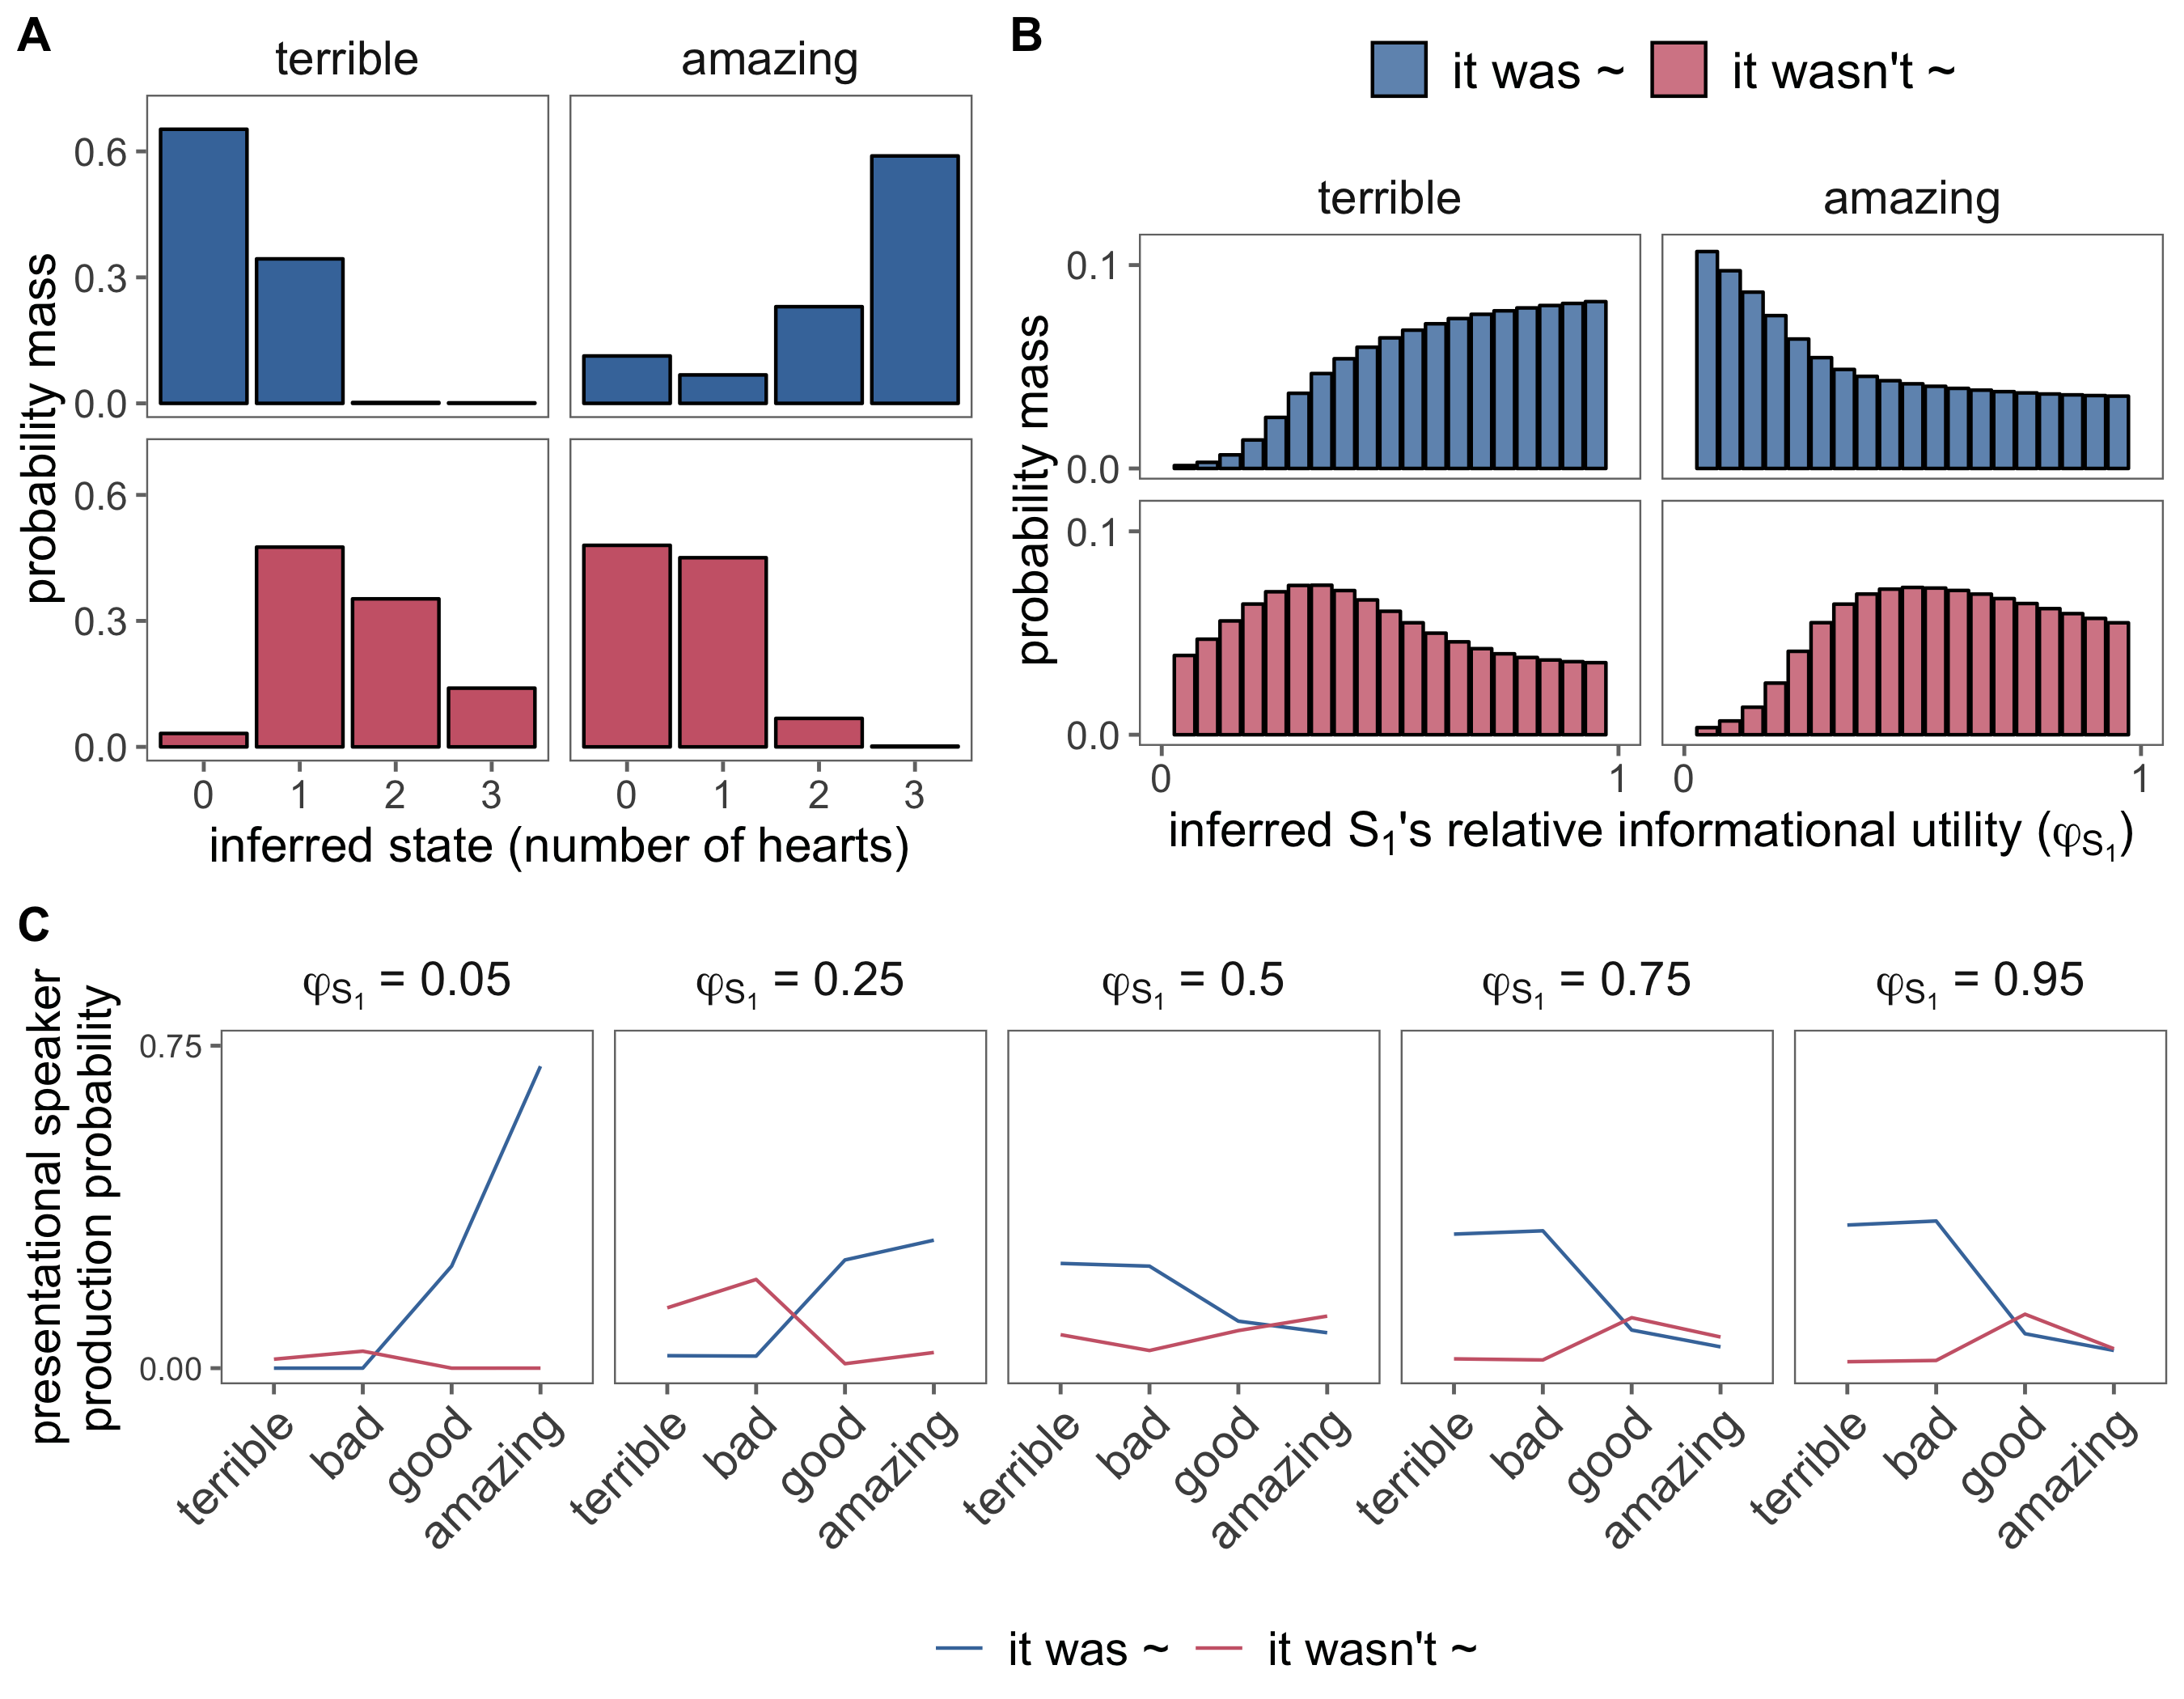
\includegraphics[width=0.9\linewidth]{/Users/ejyoon/Documents/Documents/Research/dissertation/index/chapter_child_rmds/ch4_modeling_polite/files/L1_inferences_wS2pres} 

}

\caption[Schematic predictions of the computational model.]{Model behavior. Listener inferences about the true state (e.g., the rating truly deserved by the poem; A) and the speaker's utility weighting ($\phi_{S_1}$ or how informational vs. social the speaker is, where $\phi_{S_1}$ = 0 is fully social, and $\phi_{S_1}$ = 1 is fully informational; B) as a function of the utterance heard (facets). C: Purely self-presentational speaker production behavior as a function of the kind of speaker they wish to present themselves as (facets; relatively more informational, e.g., $\phi_{S_1}$ = 0.05, vs. social as represented, e.g., $\phi_{S_1}$ = 0.95).}\label{fig:L1inferences}
\end{figure}
\section{Model predictions}\label{model-predictions}

The pragmatic listener model \(L_1\) draws complex inferences about both
the true state of the world (Fig.~\ref{fig:L1inferences}A) and the
speaker's goals (Fig.~\ref{fig:L1inferences}B). Upon hearing
\emph{{[}Your poem{]} was terrible} (Fig.~\ref{fig:L1inferences}A
and~\ref{fig:L1inferences}B top-left), the listener infers the poem is
probably truly terrible (i.e., worthy of zero hearts) and that the
speaker has strong informational goals. \emph{It was amazing} is more
ambiguous (Figure~\ref{fig:L1inferences}A and ~\ref{fig:L1inferences}B
top-right): The poem could indeed be worthy of three hearts, but it is
also plausible the speaker had strong social goals and the poem was
mediocre. Negation makes the meanings less precise and introduces more
uncertainty into the inference about the state: A listener who hears
\emph{It wasn't amazing} sees it as a relatively kind way of saying that
the poem was quite bad (0 or 1 hearts), inferring a balance of social
and informational goals for the speaker (Figure~\ref{fig:L1inferences}A
and ~\ref{fig:L1inferences}B bottom-right). \emph{It wasn't terrible} is
the most open-ended, leaving open the possibility that the poem was
worthy of 0 hearts (i.e., \emph{it was terrible}) but conveying to the
listener that the speaker cares about both informational and social
goals, with a slight preference of towards being social
(Figure~\ref{fig:L1inferences}A and ~\ref{fig:L1inferences}B
bottom-left).

The self-presentational utility guides the speaker \(S_2\) to care about
how she will be viewed in the eyes of the listener \(L_1\)
(Figure~\ref{fig:L1inferences}C). If the speaker wants to present
herself as someone who is socially-minded (e.g., informational mixture
or \(\phi_{S_1}\) of 0.05), she should produce direct, positive
utterances (e.g., \emph{amazing}). The best way to appear honest (e.g.,
informational mixture of 0.95) is to say direct, negative utterances
(e.g., \emph{terrible}). The desire to appear as someone concerned with
telling the truth while also caring about the listener's feelings (e.g.,
\(\phi_{S_1}\) of 0.25) leads the speaker to produce indirect utterances
(e.g., \emph{not terrible}). Such indirect speech acts are sufficiently
open-ended to include the possibility that the poem was good, but the
avoidance of a more direct utterance (e.g., \emph{good}) provides the
listener with a way to recover the true state (e.g., the poem was
mediocre) by way of reasoning that the speaker cares about his feelings
by not saying the blunt truth.

\section{Experiment: Speaker production
task}\label{experiment-speaker-production-task}

We made a direct, fully pre-registered test of our speaker production
model and its performance in comparison to a range of alternative
models, by instantiating our running example in an online experiment.
\begin{figure}[!h]

{\centering 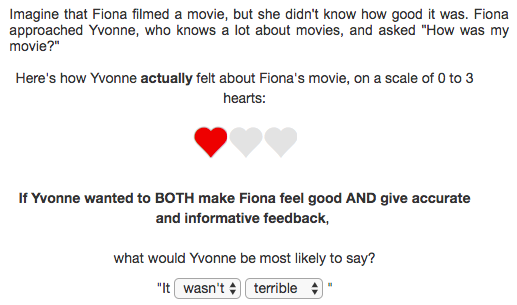
\includegraphics[width=0.9\linewidth]{/Users/ejyoon/Documents/Documents/Research/dissertation/index/chapter_child_rmds/ch4_modeling_polite/files/screenshot} 

}

\caption[Example of a trial in the experimental task in Chapter 4.]{Example of a trial in the speaker production task.}\label{fig:screenshot}
\end{figure}
\subsection{Participants}\label{participants-4}

202 participants with IP addresses in the United States were recruited
on Amazon's Mechanical Turk.

\subsection{Design and Methods}\label{design-and-methods}

Participants read scenarios with information on the speaker's feelings
toward some performance or product (e.g., a poem recital; \emph{true
state}), on a scale from zero to three hearts (e.g., one out of three
hearts). For example, one trial read: \emph{Imagine that Bob gave a poem
recital, but he didn't know how good it was. Bob approached Ann, who
knows a lot about poems, and asked} ``How was my poem?'' Additionally,
we manipulated the speaker's goals across trials: to be
\emph{informative} (``give accurate and informative feedback''); to be
\emph{kind} (``make the listener feel good''); or to be \emph{both}
informative and kind simultaneously. We hypothesized that each of the
three experimentally-induced goals would induce a different tradeoff
between social and informational utilities in our model, as well as
modulating the self-presentational component. In a single trial, each
scenario was followed by a question asking for the most likely produced
utterance by Ann. Participants selected one of eight possible
utterances, by choosing between \emph{It was} vs. \emph{It wasn't} and
then among \emph{terrible}, \emph{bad}, \emph{good}, and \emph{amazing.}

Each participant read twelve scenarios, depicting every possible
combination of the three goals and four states. The order of context
items was randomized, and there were a maximum of two repeats of each
context item per participant. Each scenario was followed by a question
that read, ``If Ann wanted to make Bob feel good but not necessarily
give informative feedback (or to give accurate and informative feedback
but not necessarily make Bob feel good, or BOTH make Bob feel good AND
give accurate and informative feedback), what would Ann be most likely
to say?'' Participants indicated their answer by choosing one of the
options on the two dropdown menus, side-by-side, one for choosing
between \emph{It was} vs. \emph{It wasn't} and the other for choosing
among \emph{terrible}, \emph{bad}, \emph{good}, and \emph{amazing.}

\subsection{Behavioral results}\label{behavioral-results}
\begin{figure}[!t]

{\centering 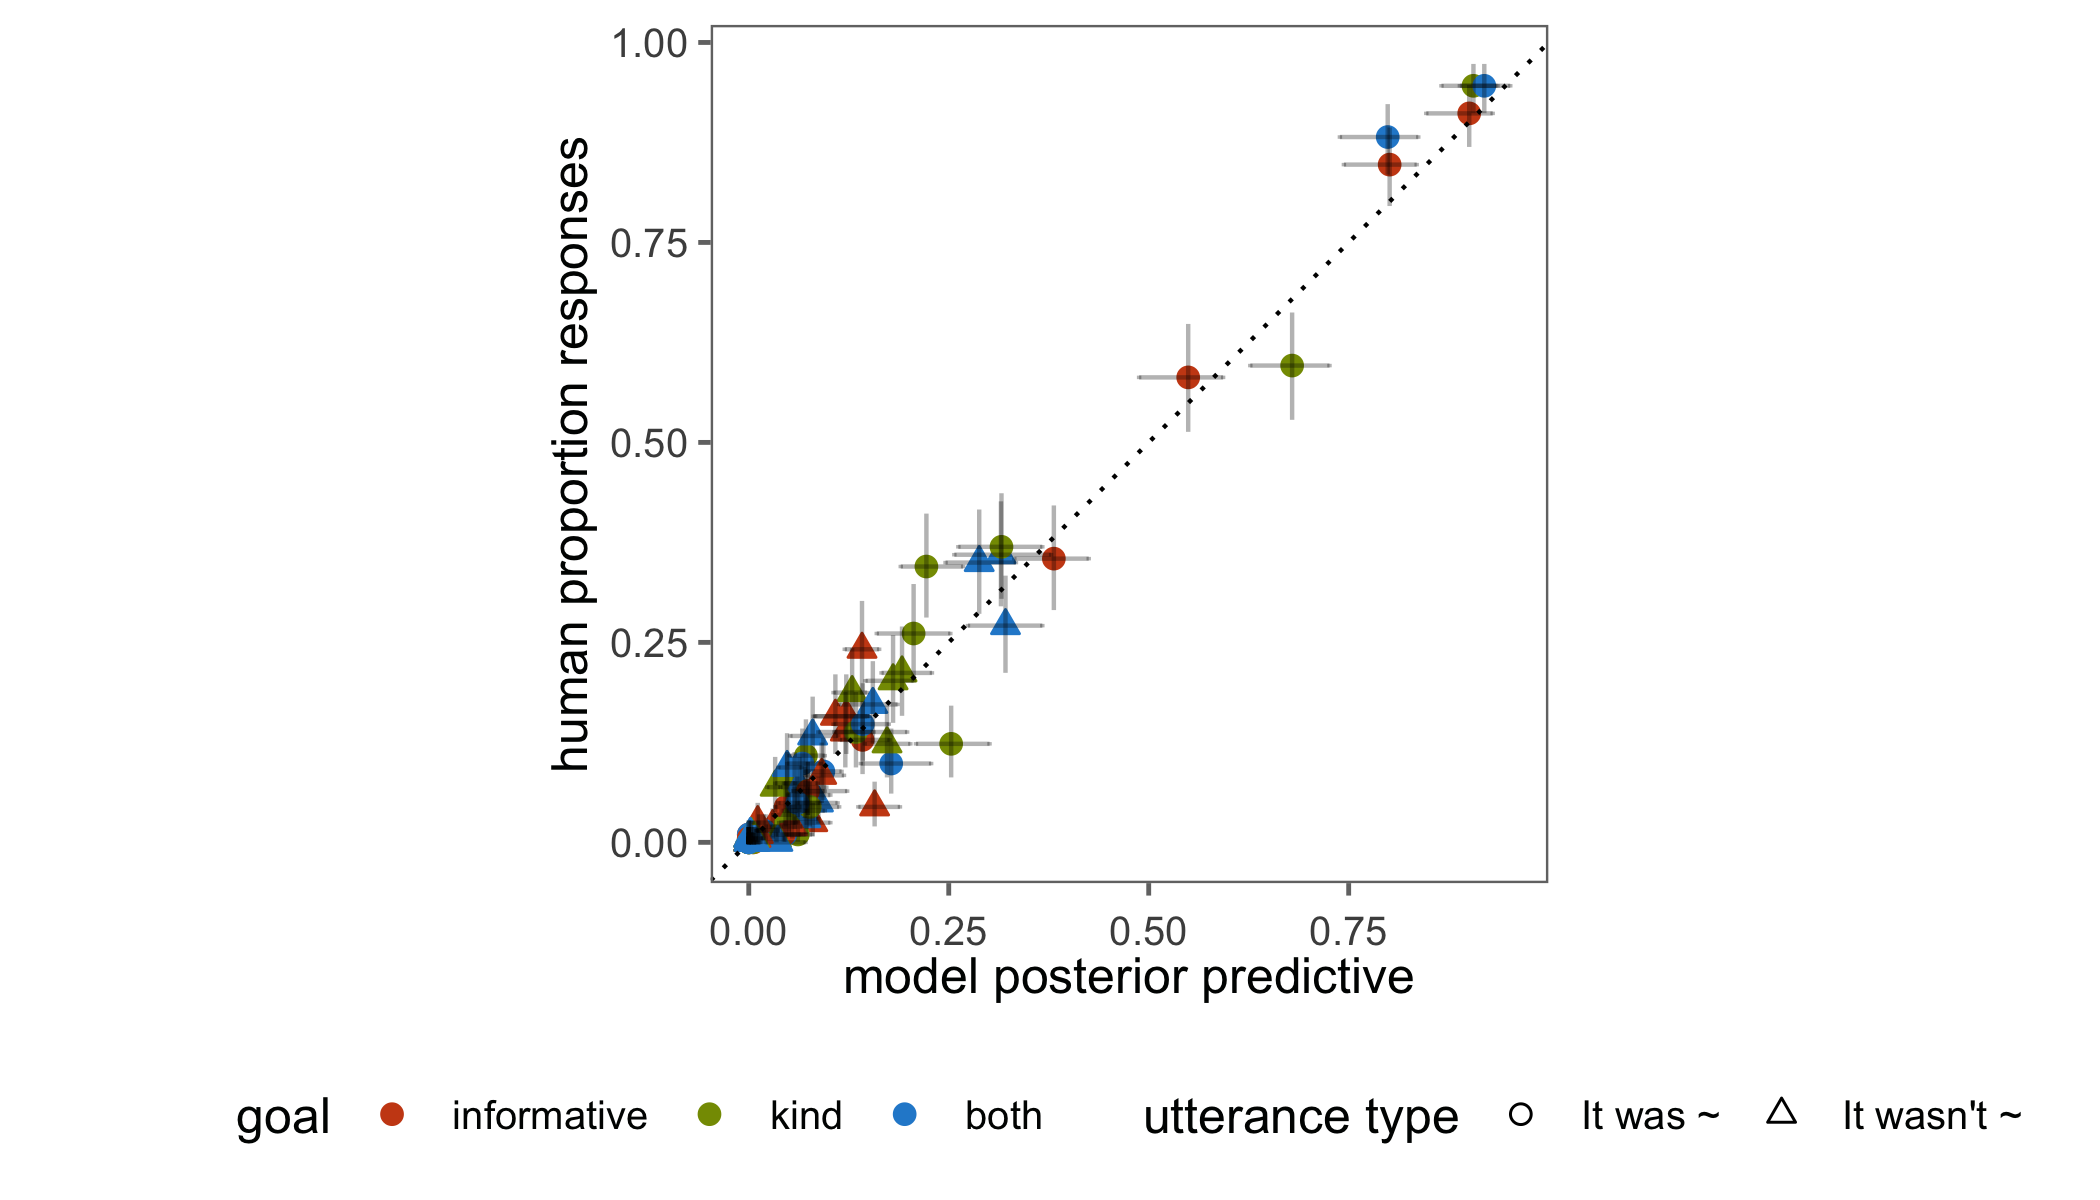
\includegraphics[width=0.9\linewidth]{/Users/ejyoon/Documents/Documents/Research/dissertation/index/chapter_child_rmds/ch4_modeling_polite/files/speaker_production_cor} 

}

\caption[Comparison between model predictions and human responses from Experiment in Chapter 4.]{Full distribution of human responses vs. model predictions. Error bars represent 95\% confidence intervals for the data (vertical) and 95\% highest density intervals for the model (horizontal).}\label{fig:variance}
\end{figure}
Our primary behavioral hypothesis was that speakers describing bad
states (e.g., poem deserving 0 hearts) with goals to be both informative
and kind would produce more indirect, negative utterances (e.g.,
\emph{It wasn't terrible}). Such indirect speech acts both save the
listener's face and provide some information about the true state, and
thus, are what a socially-conscious speaker would say
(Figure~\ref{fig:L1inferences}). This prediction was confirmed, as a
Bayesian mixed-effects model predicts more negation as a function of
true state and goal via an interaction: A speaker with both goals to be
informative and kind produced more negation in worse states compared to
a speaker with only the goal to be informative (\emph{M} = -1.33,
{[}-1.69, -0.98{]}) and goal to be kind (\emph{M} = -0.5, {[}-0.92,
-0.07{]}). Rather than eschewing one of their goals to increase utility
along a single dimension, participants chose utterances that jointly
satisfied their conflicting goals by producing indirect speech.
\begin{figure}[!t]

{\centering 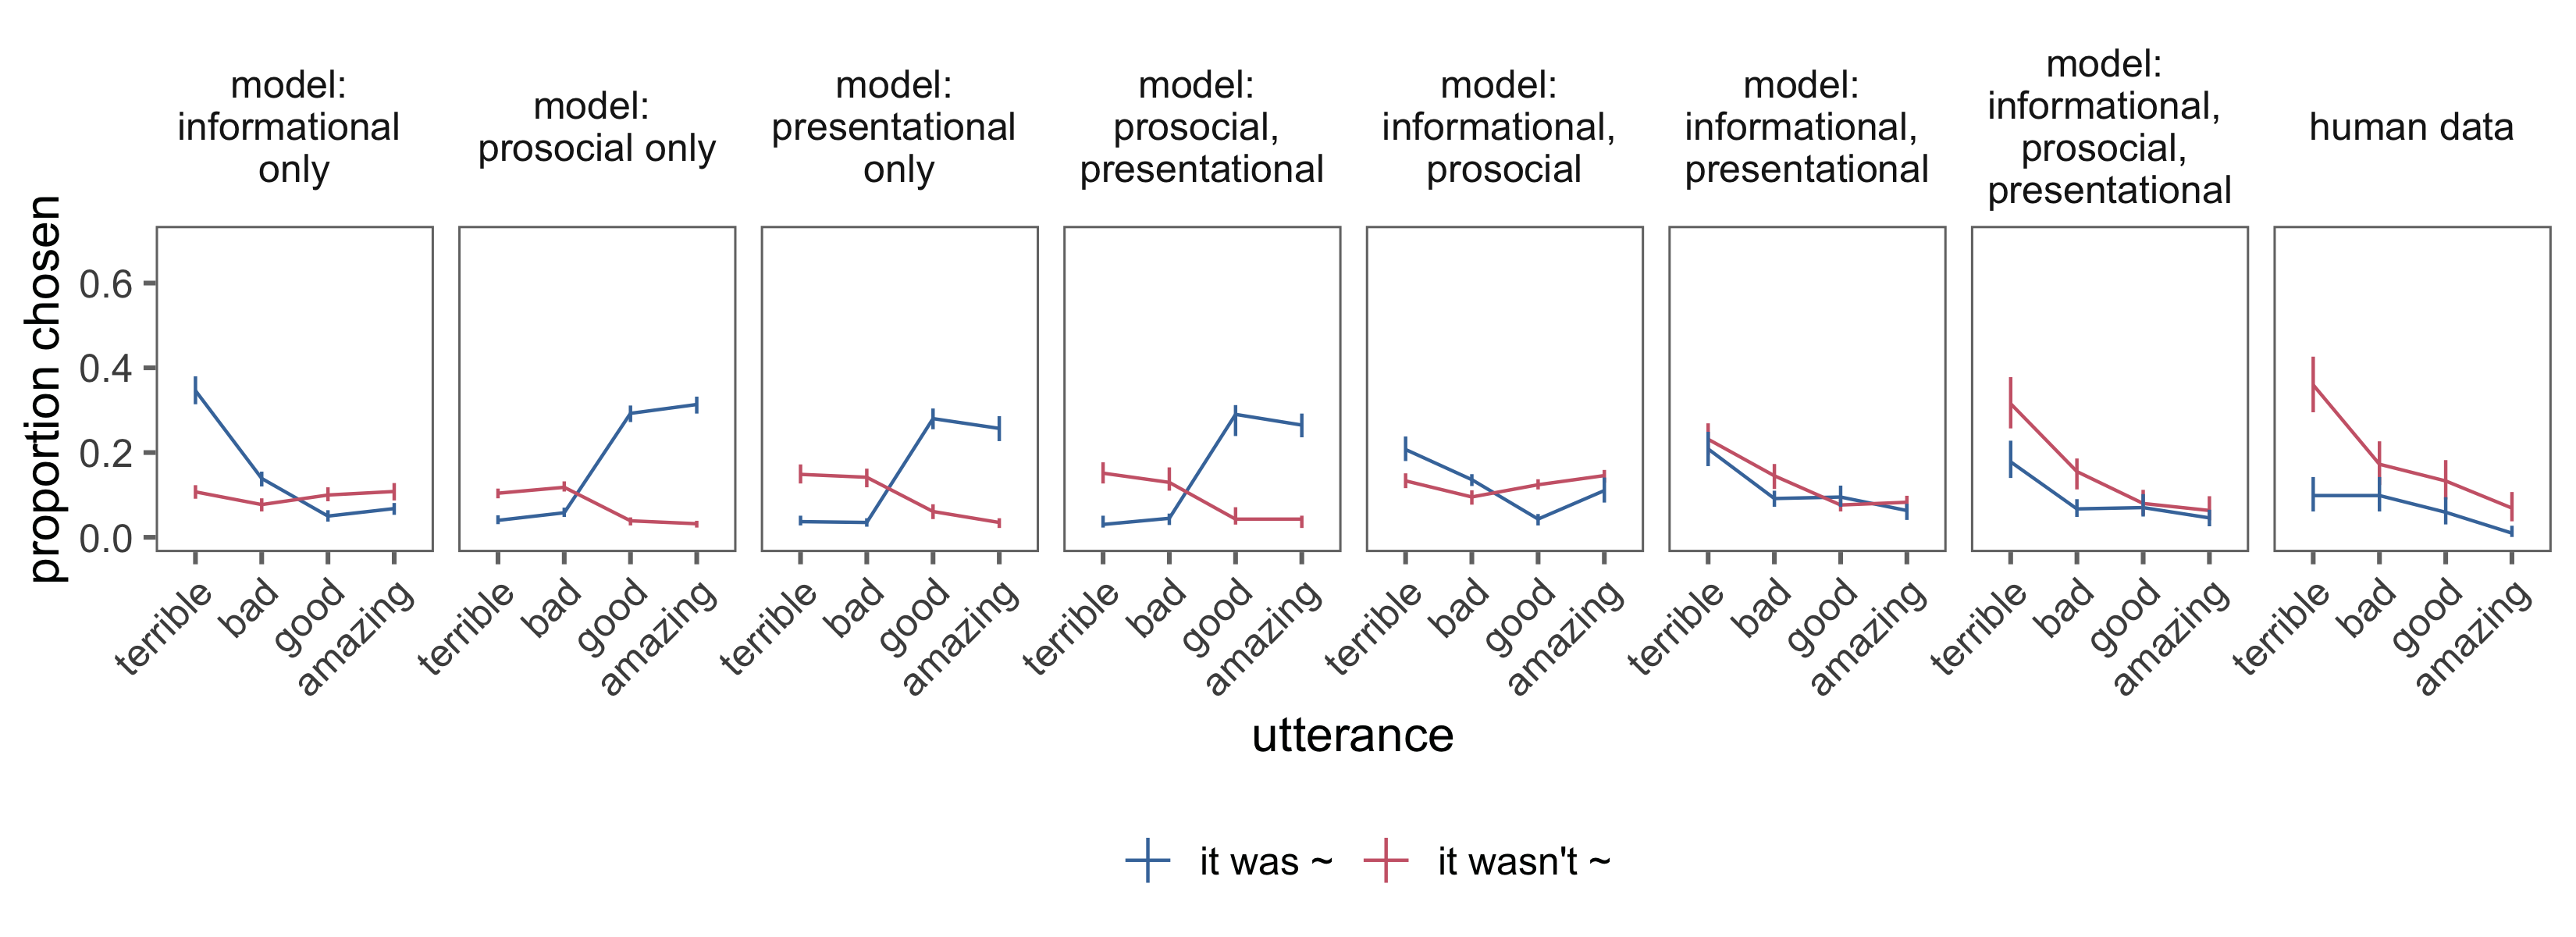
\includegraphics[width=0.9\linewidth]{/Users/ejyoon/Documents/Documents/Research/dissertation/index/chapter_child_rmds/ch4_modeling_polite/files/model_comparisons} 

}

\caption[Comparison of computational model variant fits.]{Comparison of predictions for proportion of utterances chosen by pragmatic speaker from possible model variants (left) and human data (rightmost) for average proportion of negation produced among all utterances, given true state of 0 heart (on a scale of 0 to 3) and speaker with both goals to be informative and kind. Gray dotted line indicates chance level at 12.5\%.}\label{fig:comparison}
\end{figure}
\begin{table}[t]

\caption[Comparison of model variants using variance explained and log Bayes Factors.]{\label{tab:comparisonTable}Comparison of variance explained for each model variant and log Bayes Factors quantifying evidence in favor of alternative model in comparison.}
\centering
\begin{tabular}{lrl}
\toprule
model & variance 
\textbf{explained} & \textbf{log BF}\\
\midrule
informational, 
social, 
presentational & 0.9712810 & --\\
informational, 
presentational & 0.9572102 & -11.14\\
informational, 
social & 0.9163242 & -25.06\\
social, 
presentational & 0.2297718 & -864\\
presentational 
only & 0.2282951 & -873.83\\
\addlinespace
social only & 0.2169990 & -885.52\\
informational 
only & 0.8332508 & -274.89\\
\bottomrule
\end{tabular}
\end{table}
\subsection{Model results}\label{model-results}

The model parameters (softmax parameters and each goal condition's
utility weights) can be inferred from the behavioral data using Bayesian
data analysis (M. D. Lee \& Wagenmakers, 2014). To approximate the
literal meanings (i.e., the semantics) of the words as interpreted by
the literal listener \(L_0\), we obtained literal meaning judgments from
an independent group of participants (See Supplmentary Materials:
Literal semantic task section). The posterior predictions from the the
three-utility polite speaker model (informational, social,
presentational) showed a very strong fit to participants' actual
utterance choices (\(r^2\)(96) = 0.971281; Figure~\ref{fig:variance}).
We compared these to six model variants containing subsets of the three
utilities in the full model. Both the variance explained and marginal
likelihood of the observed data were the highest for the full model
(Table~\ref{tab:comparisonTable}). Only the full model captured
participants' preference for negation when the speaker wanted to be
informative and kind about truly bad states, as hypothesized
(Figure~\ref{fig:comparison}). In sum, the full set of informational,
social, and presentational were required to fully explain participants'
utterance choices.
\begin{table}[t]

\caption[Inferred phi parameters from model variants.]{\label{tab:phi}Inferred phi parameters from all model variants with more than one utility.}
\centering
\begin{tabular}{llllll}
\toprule
\textbf{model (utilities)} & \textbf{goal} & \textbf{$\phi_{inf}$} & \textbf{$\phi_{soc}$} & \textbf{$\phi_{pres}$} & \textbf{$\phi_{S_1}$}\\
\midrule
informational, social, presentational & both & 0.36 & 0.11 & 0.54 & 0.36\\
informational, social, presentational & informative & 0.36 & 0.02 & 0.62 & 0.49\\
informational, social, presentational & social & 0.25 & 0.31 & 0.44 & 0.37\\
informational, presentational & both & 0.64 & -- & 0.36 & 0.17\\
informational, presentational & informative & 0.77 & -- & 0.23 & 0.33\\
\addlinespace
informational, presentational & social & 0.66 & -- & 0.34 & 0.04\\
informational, social & both & 0.54 & 0.46 & -- & --\\
informational, social & informative & 0.82 & 0.18 & -- & --\\
informational, social & social & 0.39 & 0.61 & -- & --\\
social, presentational & both & -- & 0.38 & 0.62 & 0.55\\
\addlinespace
social, presentational & informative & -- & 0.35 & 0.65 & 0.75\\
social, presentational & social & -- & 0.48 & 0.52 & 0.66\\
\bottomrule
\end{tabular}
\end{table}
The utility weights inferred for the three-utility model (Table
\ref{tab:phi}) provide additional insight into how polite language use
operates in our experimental context and possibly beyond: \emph{Being
kind} (``social'') requires not only weights on social and
presentational utilities but equal weights on all three utilities,
indicating that informativity is a part of language use even when it is
explicitly not the goal. \emph{Being informative} (``informative'')
pushes the weight on social utility (\(\phi_{soc}\)) close to zero, but
the weight on \emph{appearing kind} (\(\phi_{pres}\)) stays high,
suggesting that speakers are expected to manage their own face even when
they are not considering others'. \emph{Kind and informative} (``both'')
speakers emphasize informativity slightly more than kindness. In all
cases, however, the presentational utilities have greatest weight,
suggesting that managing the listener's inferences about oneself was
integral to participants' decisions in the context of our communicative
task. Overall then, our condition manipulation altered the balance
between these weights, but all utilities played a role in all
conditions.

\section{Discussion}\label{discussion}

Politeness is puzzling from an information-theoretic perspective.
Incorporating social motivations adds a level of explanation, but so far
such intuitions and observations have resisted both formalization and
precise testing. We present a utility-theoretic model of language use
that captures the interplay between competing informational, social, and
presentational goals, and provide preregistered experimental evidence
that confirmed its ability to capture human judgments, unlike comparison
models with only a subset of the full utility structure.

To estimate precisely choice behavior in the experiment, it was required
to abstract away from natural interactions in a number of ways. Human
speakers have access to a potentially infinite set of utterances to
select from in order to manage the three-utility tradeoff (\emph{It's
hard to write a good poem}, \emph{That metaphor in the second stanza was
so relatable!}). In theory, each utterance will have strengths and
weaknesses relative to the speaker's goals, though computation in an
unbounded model presents technical challenges (perhaps paralleling the
difficulty human speakers feel in finding the right thing to say in a
difficult situation; see N. D. Goodman \& Frank, 2016).

For a socially-conscious speaker, managing listeners' inferences is a
fundamental task. Our work extends previous models of language beyond
standard informational utilities to address social and
self-presentational concerns. Further, our model builds upon the theory
of politeness as face management (P. Brown \& Levinson, 1987) and takes
a step towards understanding the complex set of social concerns involved
in face management. Our approach can provide insight into a wide range
of social behaviors beyond speech by considering utility-driven
inferences in a social context (Baker, Jara-Ettinger, Saxe, \&
Tenenbaum, 2017; Hamlin, Ullman, Tenenbaum, Goodman, \& Baker, 2013)
where agents need to take into account concerns about both self and
others.

Previous game-theoretic analyses of politeness have either required some
social cost to an utterance (e.g., by reducing one's social status or
incurring social debt to one's conversational partner; Van Rooy, 2003)
or a separately-motivated notion of plausible deniability (Pinker et
al., 2008). The kind of utterance cost for the first type of account
would necessarily involve higher-order reasoning about other agents, and
may be able to be defined in terms of the more basic social and
self-presentational goals we formalize here. A separate notion of
plausible deniability may not be needed to explain most politeness
behavior, either. Maintaining plausible deniability is in one's own
self-interest (e.g., due to controversial viewpoints or covert
deception) and goes against the interests of the addressee; some amount
of utility dis-alignment is presumed by these accounts. Politeness
behavior appears present even in the absence of obvious conflict,
however: In fact, you might be even more motivated to be polite to
someone whose utilities are more aligned with yours (e.g., a friend). In
our work here, we show that such behaviors can in fact arise from purely
cooperative goals (P. Brown \& Levinson, 1987), though in cases of
genuine conflict, plausible deniability likely plays a more central role
in communication.

Utility weights and value functions in our model could provide a
framework for a quantitative understanding of systematic cross-cultural
differences in what counts as polite. Cross-cultural differences in
politeness could be a product of different weightings within the same
utility structure. Alternatively, culture could affect the value
function \(V\) that maps states of the world onto subjective values for
the listener (e.g., the mapping from states to utilities may be
nonlinear and involve reasoning about the future). Our formal modeling
approach with systematic behavior measurements provides an avenue
towards understanding the vast range of politeness practices found
across languages.

Politeness is only one of the ways language use deviates from purely
informational transmission. We flirt, insult, boast, and empathize by
balancing informative transmissions with goals to affect others'
feelings or present particular views of ourselves. Our work shows how
social and self-presentational motives are integrated with informational
concerns more generally, opening up the possibility for a broader theory
of social language. In addition, a formal account of politeness moves us
closer to courteous computation -- to machines that can talk with tact.

\chapter*{Conclusion}\label{conclusion}
\addcontentsline{toc}{chapter}{Conclusion}

In this dissertation, I proposed a framework to unify existing theories
to understand polite language as reflecting a tradeoff between different
goals that speakers may consider. Critically, language does not only
reflect speakers' informational concerns to convey accurate information
informatively, but also non-informational social concerns, such as
following social norms and maintaining listeners' and speakers' own
positive self-image (\emph{face}). In Chapter 1, I summarized previous
approaches to polite language and argued that a goal-based framework can
integrate different components that are important to explaining how
polite speech emerges and is understood. Then I explained how existing
empirical data with adults and children that can be explained through
this goal-based framework.

In Chapters that followed, I presented evidence from our own empirical
studies that demostrated children and adults' understanding of polite
speech as reflecting a tradeoff between informational and social goals.
Chapter 2 examined 2- to 4-year-old children's understanding of social
goals behind language use, through the case study of polite requests
with simple politeness markers such as ``please,'' and ``can
you\textasciitilde{}''. By 3 years, children were able to judge that
speakers making polite requests were being more polite, and by 4 years
children were able to reason that those speakers were also likely to be
better play partners and to gain compliance to their requests.

Chapter 3 examined older children's and adults' understanding of the
tradeoff between social goals and informational goals, using the case
study of white lies (versus blunt truths). By 6 years, children seem
capable of using context information to reason about speaker goals and
make judgments about whether the speaker was being nice or mean, and
evaluate liars more positively given potential face threat to the
listener than given no apparent face threat. We saw a developmental
trend, where older children, like adults, rated polite liars more
positively whereas younger participants tended to be divided. This age
difference may be due to a discrepancy in goal priorities: Younger
children may prioritize truth-telling, which can be a simple rule to
follow (e.g., ``Don't lie, always tell the truth'') but as they get
older, they might learn to consider other people's feelings and address
the informational-social tradeoff more.

Finally, Chapter 4 examined adults' understanding of polite language in
more detail, by looking at utterance prediction in a situation of
potential face threat (e.g., speakers being asked to give feedback and
answer ``How was my poem?''), and proposed a model to formalize the
notions of speaker goals as utilities that the speaker wants to
maximize. We showed that our model predictions captured important key
patterns of human judgments, and that the model fit was superior to its
variants with a subset of the three utilities of our model. Overall, the
empirical work suggest that the goal-tradeoff framework both explains
children's and adults' understanding of polite language well, and is
useful for formalization and thus for making precise predictions of
polite speech.

There are limitations to the current theoretical framework and empirical
evidence presented in here, that have important implications for future
work. First, for the developmental work, Chapters 2 and 3 looked at
distinct age groups, 2- to 4-year-olds and 5- to 8-year-olds
respectively, making it difficult to tell how the polite speech
understanding, especially regarding the tradeoff between informational
and social goal, might develop across the entire relevant age span. For
example, do 2- to 4-year-olds show even more of preference for
prioritizing informational goals over social goals? Or do they not yet
have the notion of goal tradeoff at all? There were practical concerns
that prevented younger children's participation in the study reported in
Chapter 3, namely that it would be too difficult for younger children to
understand the stories presented in that study (due to memory demand,
tracking of second-order beliefs, etc.). It will be useful to conduct a
follow-up task that is more accessible for younger children and can test
their understanding of goal tradeoffs. It will also be helpful to
consider how children's utterance choices and evaluations may be
formalized, which will help hone explanation for the development of
polite language understanding and make precise predictions.

Second, the scope of contexts of polite speech use we explored thus far
is limited. We have not examined other factors that may be integral to
polite speech production and understanding, such as speaker-listener
status differences (e.g., conversations between a teacher and student,
instead of between friends), listener needs (e.g., listener is looking
for feedback to enter a competition), and available utterances (e.g.,
other kinds of indirect speech such as ``I don't think this cookie is
very tasty''). Thus, it is an open question whether and how children and
adults process these other kinds of relevant information and integrate
them into their understanding of polite utterances.

Also, here we addressed broadly three differentiable goals --
informational, prosocial, and self-presentational -- that speakers may
consider, but in real life, there may be other goals that are important,
or these goals may also be broken down further. For example, in the
current work we supposed that speakers consider self-presentational
goals to appear informative or to appear kind, but depending on the
context, speakers may care about appearing competent and knowledgeable.
Indeed, people do account for this kind of presentational goal to
determine their action in a social active learning context, where they
must choose between maximal information gain (e.g., learn which button
makes a machine work) versus presentation of oneself as competent (e.g.,
that they can make the machine work for sure; Yoon, MacDonald, Asaba,
Gweon, \& Frank, 2018). Thus, future work should investigate how
different desires than ones examined here may play roles in speakers'
utterance choices.

Finally, the empirical studies presented here recruited participants in
the US only, but there may be great variations in polite speech
understanding depending on cultural norms and expectations. For example,
some cultures and languages may emphasize prosocial goals more than
informational goals and thus have expectations for speakers to
prioritize kindness over informativity, whereas other cultures might
value truthfulness as a greater virtue than face-saving. Indeed, we have
some preliminary evidence that Indian speakers, both adults and
children, value informational goals more and are more charitable toward
blunt truth-tellers than polite liars compared to US and Korean
speakers. Formalisation and empirical test of these cultural variations
will help further the understanding of polite language.

In sum, I argued for a goal-based framework for polite language
understanding, in which speakers consider tradeoffs between
informational and social concerns. Our empirical research shows that
adults and children are sensitive to not only informational goals but
also social goals behind language use, and consider tradeoffs between
these goals when reasoning about speakers' utterance choices. I also
presented a formal model of the goal tradeoffs, which allowed for
precise quantitative predictions that matched human adults' polite
speech predictions well. This theoretical approach accompanied by
computational framework then can be a powerful tool in addressing
possible future work to extend on many other factors that must be
considered to explain human understanding of polite language, and
pragmatics and social behaviors in general.

\appendix

\chapter{Supplementary materials for Chapter
3}\label{supplementary-materials-for-chapter-3}

\section{Stimuli}\label{stimuli-1}

\subsection{Training trial}\label{training-trial}

Nicole gave her friend a gift. Was Nicole nice? Was Nicole mean?

James hit his friend. Was James nice? Was James mean?

Kyle broke his mom's vase, and he told his mom the truth that he broke
it. Was Kyle telling the truth?

Pam ate five cookies, but Pam told her mom a lie that she didn't eat any
cookie. Was Pam telling the truth?

\subsection{Example test story (experimental
condition)}\label{example-test-story-experimental-condition}

Look, this is Edward! One day, Edward decided to bake some cookies.
Edward brought his cookie to school and met his friend Sally. Edward
said to his friend Sally, ``Here, try my cookie!'' Sally tasted the
cookie, and she did not like the cookie at all --- she thought the
cookie tasted yucky! So did Sally like the cookie or did she not like
the cookie?

Edward asked Sally, ``Sally, how did you like my cookie?'' Sally told
Edward, ``Edward, your cookie was tasty.'' So what did Sally tell Edward
again?

Let's think about the story again. Sally thought the cookie was yucky.
And Sally told Edward that the cookie was yucky. Was Sally nice? Was
Sally mean? Was Sally telling the truth?

Look, this is Edward again! One day, Edward decided to bake some
cookies. Edward brought his cookie to school and met his friend Mary.
Edward said to his friend Mary, ``Here, try my cookie!'' Mary tasted the
cookie, and she did not like the cookie at all --- she thought the
cookie tasted yucky! So did Mary like the cookie or did she not like the
cookie?

Edward asked Mary, ``Mary, how did you like my cookie?'' Mary told
Edward, ``Edward, your cookie was tasty.'' So what did Mary tell Edward
again?

Let's think about the story again. Mary thought the cookie was yucky.
And Mary told Edward that the cookie was tasty. Was Mary nice? Was Mary
mean? Was Mary telling the truth?

Remember Sally and Mary from our story? Look, here they are. Remember,
Sally thought the cookie was yucky and told Edward that the cookie was
yucky. Mary thought the cookie was yucky and told Edward that the cookie
was tasty. Who do you want to play with more, Sally or Mary? Why?

\subsection{Example test story (control
condition)}\label{example-test-story-control-condition}

Look, this is Sally! One day, Sally saw a free cookie. Sally said,
``It's a free cookie, I'll try it!'' Sally tasted the cookie, and she
did not like the cookie at all --- she thought the cookie tasted yucky!
So did Sally like the cookie or did she not like the cookie?

Sally's friend Edward also wanted to taste the cookie. Edward asked
Mary, ``Sally, how did you like the cookie?'' Sally told Edward,
``Edward, the cookie was yucky.'' So what did Sally tell Edward again?

Let's think about the story again. Sally thought the cookie was yucky.
And Sally told Edward that the cookie was yucky Was Sally nice? Was
Sally mean? Was Sally telling the truth?

Look, this is Mary! One day, Mary saw a free cookie. Mary said, ``It's a
free cookie, I'll try it!'' Mary tasted the cookie, and she did not like
the cookie at all --- she thought the cookie tasted yucky! So did Mary
like the cookie or did she not like the cookie?

Mary's friend Edward also wanted to taste the cookie. Edward asked Mary,
``Mary, how did you like the cookie?'' Mary told Edward, ``Edward, the
cookie was tasty.'' So what did Mary tell Edward again?

Let's think about the story again. Mary thought the cookie was yucky.
And Mary told Edward that the cookie was tasty. Was Mary nice? Was Mary
mean? Was Mary telling the truth?

Remember Sally and Mary from our story? Look, here they are. Remember,
Sally thought the cookie was yucky and told Edward that the cookie was
yucky. Mary thought the cookie was yucky and told Edward that the cookie
was tasty. Who do you want to play with more, Sally or Mary? Why?

\section{Supplemental figure}\label{supplemental-figure}
\begin{figure*}[p]

{\centering 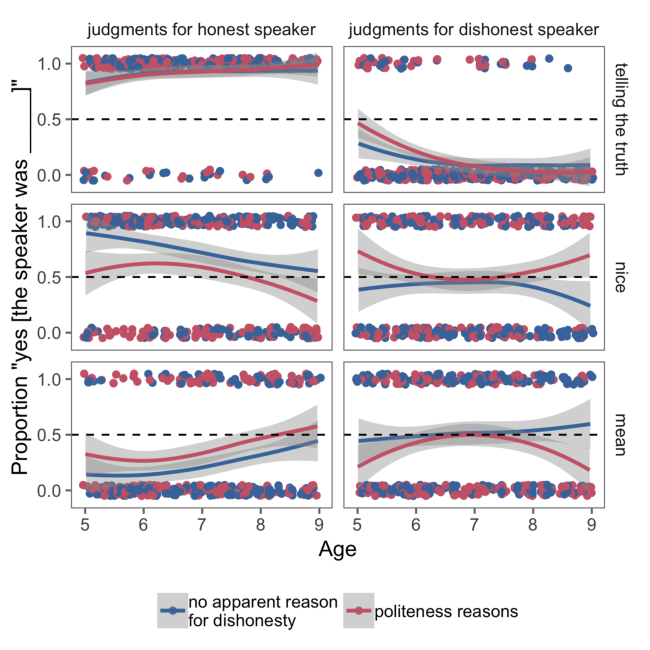
\includegraphics[width=0.9\linewidth]{erica_yoon_dissertation_files/figure-latex/figTrupolAppendix-1} 

}

\caption[Speaker ratings for the experiment in Chapter 4 with age as a continuous variable.]{Speaker judgments by participants of different age (x-axis) for the honest speaker (left column) and the dishonest speaker (right), in different contexts (colors). Rows represent question types (e.g., Was Sally telling the truth?), and y-axis represents proportion saying ``yes" to the question. Each point represents a participant response in a trial.}\label{fig:figTrupolAppendix}
\end{figure*}
\chapter{Supplementary materials for Chapter
4}\label{supplementary-materials-for-chapter-4}

\section{Model details}\label{model-details}

The \emph{literal listener} \(L_0\) is a simple Bayesian agent that
takes the utterance to be true:

\[P_{L_0}(s | w) \propto [\![ w ]\!] (s) * P(s).\]

\noindent where \([\![ w ]\!](s)\) is the truth-functional denotation of
the utterance \(w\) (i.e.~the utterance's literal meaning): It is a
function that maps world-states \(s\) to Boolean truth values. The
literal meaning is used to update the literal listener's prior beliefs
over world states \(P(s)\).

The \emph{speaker} \(S_1\) chooses utterances approximately optimally
given a utility function, which can be decomposed into two components.
First, informational utility (\(U_{inf}\)) is the amount of information
a literal listener \(L_0\) would still not know about world state \(s\)
after hearing a speaker's utterance \(w\). Second, social utility
(\(U_{soc}\)) is the expected subjective utility of the state inferred
given the utterance \(w\). The utility of an utterance subtracts the
cost \(c(w)\) from the weighted combination of the social and epistemic
utilities.

\[U(w; s; \phi_{S_1}) = \phi_{S_1} \cdot \ln(P_{L_0}(s \mid w)) + (1 - \phi_{S_1}) \cdot \mathbb{E}_{P_{L_0}(s \mid w)}[V(s)] - C(w).\]

\noindent The speaker then chooses utterances \(w\) softmax-optimally
given the state \(s\) and his goal weight mixture \(\phi_{S_1}\):

\[P_{S_1}(w \mid s, \phi_{S_1}) \propto \mathrm{exp}(\lambda_{1} \cdot \mathbb{E}[U(w; s; \phi_{S_1})]).\]

\section{Literal semantic task}\label{literal-semantic-task}

We probed judgments of literal meanings of the target words assumed by
our model and used in our main experiment.

\subsection{Participants}\label{participants-5}

51 participants with IP addresses in the United States were recruited on
Amazon's Mechanical Turk.

\subsection{Design and Methods}\label{design-and-methods-1}

We used thirteen different context items in which a speaker evaluated a
performance of some kind. For example, in one of the contexts, Ann saw a
presentation, and Ann's feelings toward the presentation (true state)
were shown on a scale from zero to three hearts (e.g., two out of three
hearts filled in red color; see Figure~\ref{fig:screenshot} for an
example of the heart scale). The question of interest was ``Do you think
Ann thought the presentation was / wasn't X?'' and participants
responded by choosing either ``no'' or ``yes.'' The target could be one
of four possible words: \emph{terrible}, \emph{bad}, \emph{good}, and
\emph{amazing}, giving rise to eight different possible utterances (with
negation or no negation). Each participant read 32 scenarios, depicting
every possible combination of states and utterances. The order of
context items was randomized, and there were a maximum of four repeats
of each context item per participant.

\subsection{Behavioral results}\label{behavioral-results-1}

We analyzed the data by collapsing across context items. For each
utterance-state pair, we computed the posterior distribution over the
semantic weight (i.e., how consistent X utterance is with Y state)
assuming a uniform prior over the weight (i.e., a standard Beta-Binomial
model). Meanings of the words as judged by participants were as one
would expect (Figure~\ref{fig:litsem}).
\begin{figure}[!h]

{\centering 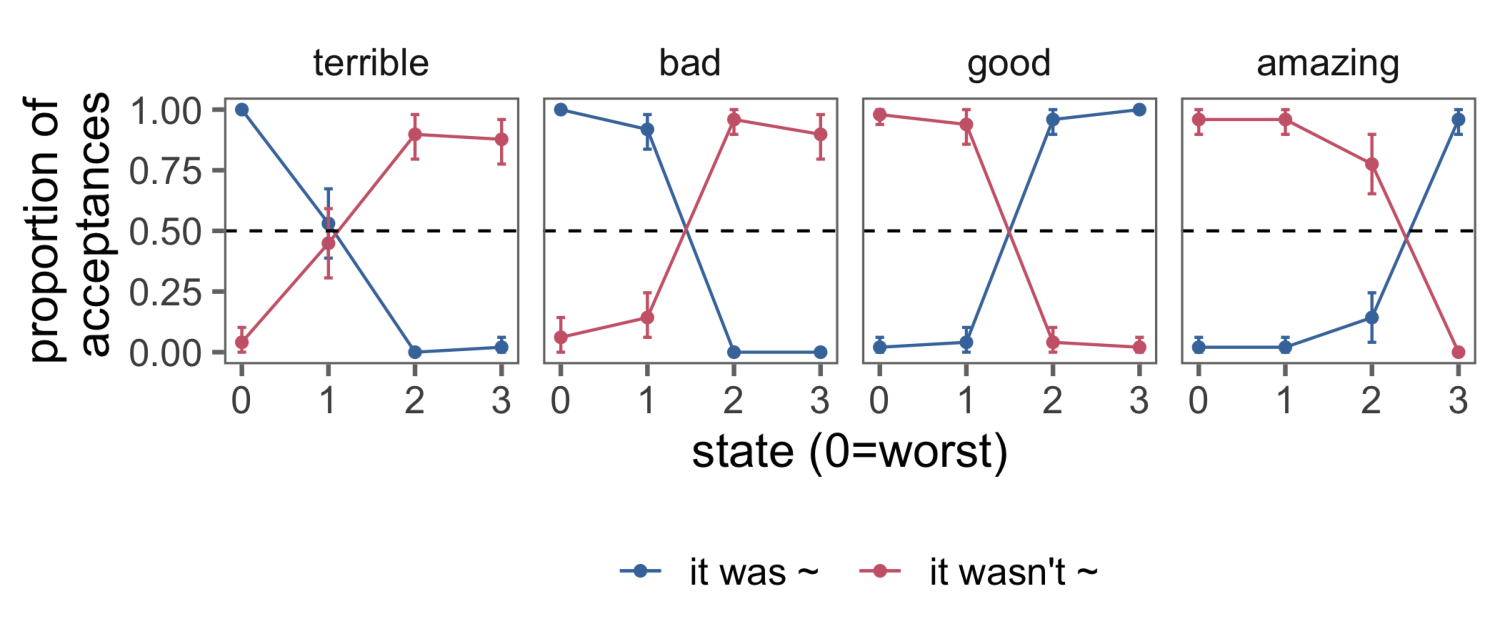
\includegraphics[width=\textwidth]{erica_yoon_dissertation_files/figure-latex/litsemPlotPlacement-1} 

}

\caption[Semantic measurement results for Chapter 4.]{Semantic measurement results. Proportion of acceptances of utterance types (shown in different colors) combined with target words (shown in different facets) given the true state represented on a scale of hearts. Error bars represent 95\% confidence intervals.}\label{fig:litsemPlotPlacement}
\end{figure}
\section{Data analysis}\label{data-analysis}

We used R (Version 3.4.3; R Core Team, 2017) and the R-packages
\emph{BayesFactor} (Version 0.9.12.2; Morey \& Rouder, 2015),
\emph{bindrcpp} (Version 0.2.2; Müller, 2017a), \emph{binom} (Version
1.1.1; Dorai-Raj, 2014), \emph{brms} (Version 2.0.1; B��rkner, 2017),
\emph{coda} (Version 0.19.1; Plummer, Best, Cowles, \& Vines, 2006),
\emph{directlabels} (Version 2017.3.31; Hocking, 2017), \emph{dplyr}
(Version 0.8.0.1; Wickham, Francois, Henry, \& Müller, 2017),
\emph{forcats} (Version 0.2.0; Wickham, 2017a), \emph{ggplot2} (Version
3.0.0; Wickham, 2009), \emph{ggthemes} (Version 3.4.0; Arnold, 2017),
\emph{gridExtra} (Version 2.3; Auguie, 2017), \emph{here} (Version 0.1;
Müller, 2017b), \emph{jsonlite} (Version 1.6; Ooms, 2014),
\emph{langcog} (Version 0.1.9001; Braginsky, Yurovsky, \& Frank, n.d.),
\emph{lme4} (Version 1.1.15; D. Bates, Mächler, Bolker, \& Walker,
2015), \emph{magrittr} (Version 1.5; Bache \& Wickham, 2014),
\emph{Matrix} (Version 1.2.12; D. Bates \& Maechler, 2017),
\emph{papaja} (Version 0.1.0.9655; Aust \& Barth, 2017), \emph{purrr}
(Version 0.2.5; Henry \& Wickham, 2017), \emph{RColorBrewer} (Version
1.1.2; Neuwirth, 2014), \emph{Rcpp} (Eddelbuettel \& Balamuta, 2017;
Version 1.0.1; Eddelbuettel \& François, 2011), \emph{readr} (Version
1.1.1; Wickham, Hester, \& Francois, 2017), \emph{rwebppl} (Version
0.1.97; Braginsky, Tessler, \& Hawkins, n.d.), \emph{stringr} (Version
1.3.1; Wickham, 2017b), \emph{tibble} (Version 2.1.1; Müller \& Wickham,
2017), \emph{tidyr} (Version 0.7.2; Wickham \& Henry, 2017), and
\emph{tidyverse} (Version 1.2.1; Wickham, 2017c) for all our analyses.

\section{Full statistics on human
data}\label{full-statistics-on-human-data}
\begin{table}[tbp]
\begin{center}
\begin{threeparttable}
\caption{\label{tab:brmTab}Predictor mean estimates with standard deviation and 95\% credible interval information for a Bayesian linear mixed-effects model predicting negation production based on true state and speaker goal (with both-goal as the reference level).}
\begin{tabular}{lllll}
\toprule
Predictor & \multicolumn{1}{c}{Mean} & \multicolumn{1}{c}{SD} & \multicolumn{1}{c}{95\% CI-Lower} & \multicolumn{1}{c}{95\% CI-Upper}\\
\midrule
Intercept & 0.88 & 0.13 & 0.63 & 1.12\\
True state & 2.18 & 0.17 & 1.86 & 2.53\\
Goal: Informative & 0.47 & 0.17 & 0.14 & 0.80\\
Goal: Kind & 0.97 & 0.25 & 0.51 & 1.49\\
True state * Informative & -1.33 & 0.18 & -1.69 & -0.98\\
True state * Kind & -0.50 & 0.22 & -0.92 & -0.07\\
\bottomrule
\end{tabular}
\end{threeparttable}
\end{center}
\end{table}
We used Bayesian linear mixed-effects models (\texttt{brms} package in
R; B��rkner, 2017) using crossed random effects of true state and goal
with maximal random effects structure (Barr et al., 2013b; A. Gelman \&
Hill, 2006). The full statistics are shown in Table \ref{tab:brmTab}.

\section{Model fitting and inferred
parameters}\label{model-fitting-and-inferred-parameters}
\begin{table}[t]

\caption[Other inferred parameters for all model variants.]{\label{tab:otherParams}Inferred negation cost and speaker optimality parameters for all model variants.}
\centering
\begin{tabular}{lrr}
\toprule
\textbf{Model} & \textbf{Cost of negation} & \textbf{Speaker optimality}\\
\midrule
informational only & 1.58 & 8.58\\
informational, presentational & 1.89 & 2.93\\
informational, social & 1.11 & 3.07\\
informational, social, presentational & 2.64 & 4.47\\
presentational only & 2.58 & 9.58\\
\addlinespace
social only & 1.73 & 7.23\\
social, presentational & 2.49 & 5.29\\
\bottomrule
\end{tabular}
\end{table}
Other than speaker goal mixture weights explained in the main text
(shown in Table \ref{tab:phi}), the full model has two global
parameters: the speaker's soft-max parameter \(\lambda_{S_2}\) and
soft-max paramater of the hypothetical speaker that the pragmatic
listener reasons about \(\lambda_{S_1}\). \(\lambda_{S_1}\) was 1, and
\(\lambda_{S_2}\) was inferred from the data: We put a prior that was
consistent with those used for similar models in this model class:
\(\lambda_{S_2}\) \textasciitilde{} \(Uniform(0,20)\). Finally, we
incorporate the literal semantics data into the RSA model by maintaining
uncertainty about the semantic weight of utterance \(w\) for state
\(s\), for each of the states and utterances, and assuming a
Beta-Binomial linking function between these weights and the literal
semantics data (see \emph{Literal semantics task} above). We infer the
posterior distribution over all of the model parameters and generate
model predictions based on this posterior distribution using Bayesian
data analysis (M. D. Lee \& Wagenmakers, 2014). We ran 4 MCMC chains for
80,000 iterations, discarding the first 40,000 for burnin. The inferred
values of parameters are shown in Table \ref{tab:otherParams}.

\section{Data Availability}\label{data-availability}

Our model, preregistration of hypotheses, procedure, data, and analyses
are available at \url{https://github.com/ejyoon/polite_speaker}.

\section{Supplemental Figures}\label{supplemental-figures}
\begin{figure}[!h]

{\centering 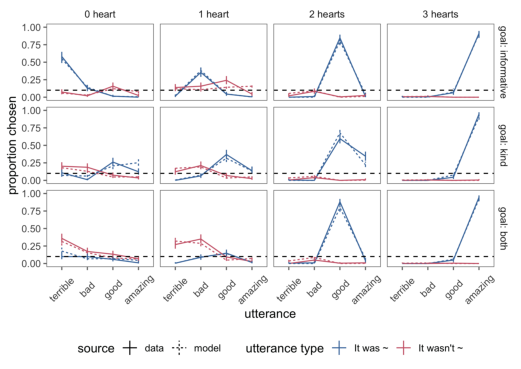
\includegraphics[width=\textwidth]{erica_yoon_dissertation_files/figure-latex/utterancePlacement-1} 

}

\caption[Full comparison between model predictions and experimental results from Chapter 4.]{Experimental results (solid lines) and fitted predictions from the full model (dashed lines) for speaker production. Proportion of utterances chosen (utterance type – direct vs. indirect – in different colors and words shown on x-axis) given the true states (columns) and speaker goals (rows). Error bars represent 95\% confidence intervals for the data and 95\% highest density intervals for the model. Black dotted line represents the chance level.}\label{fig:utterancePlacement}
\end{figure}
\begin{figure}[!h]

{\centering 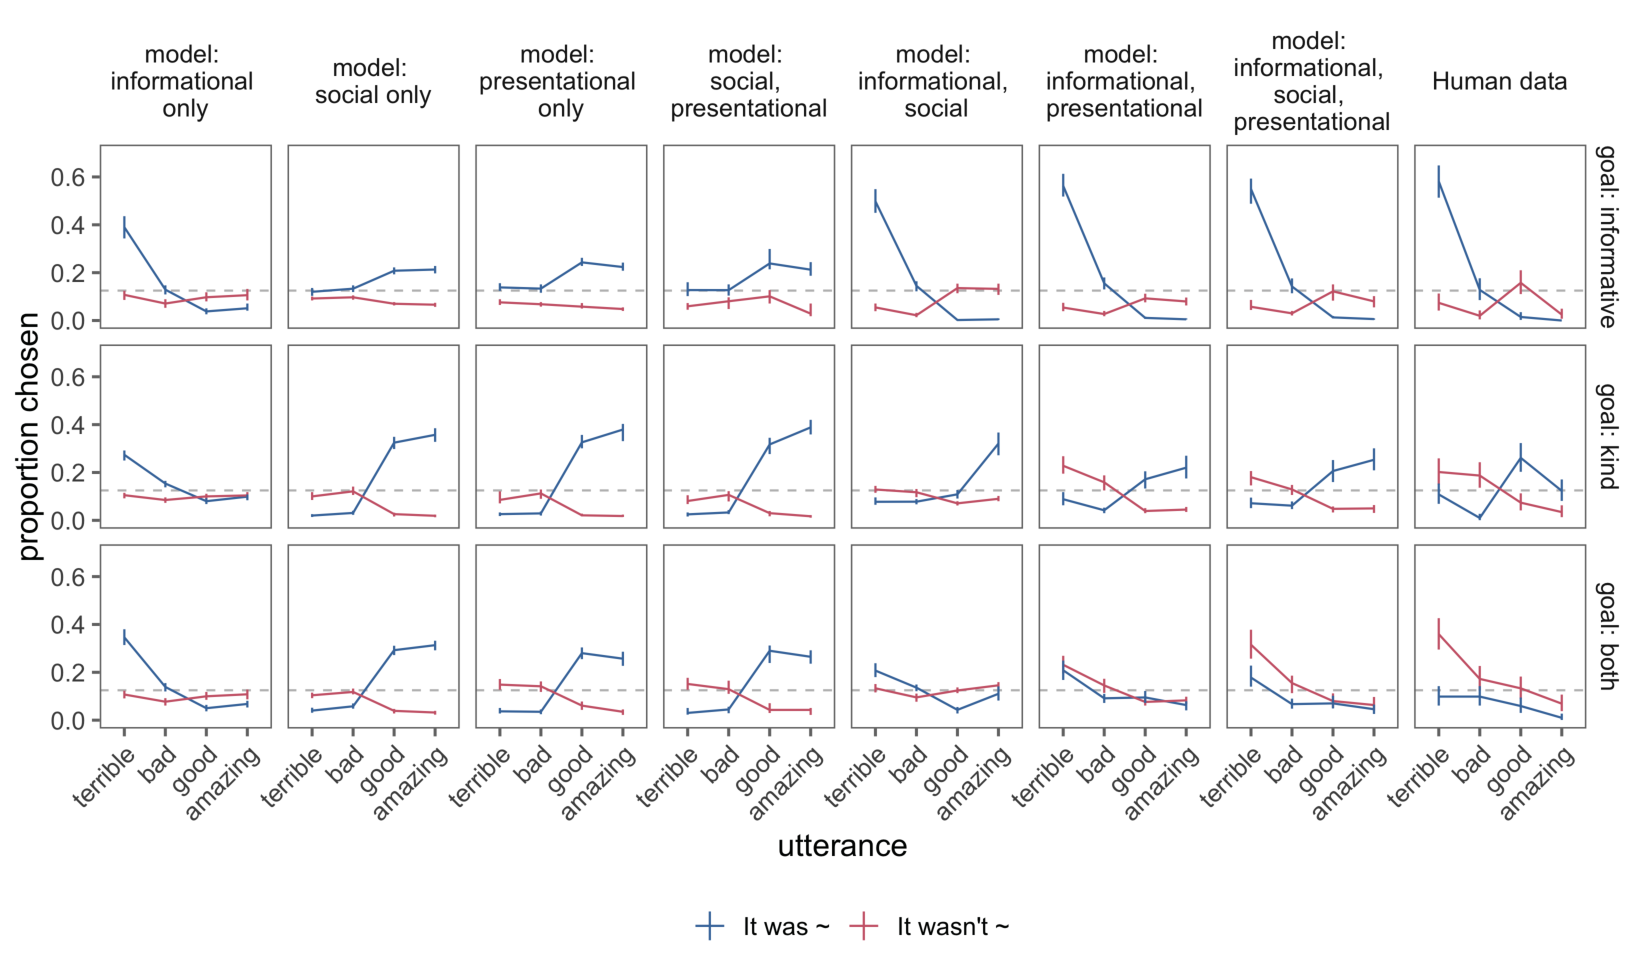
\includegraphics[width=\textwidth]{erica_yoon_dissertation_files/figure-latex/comparisonAllPlacement-1} 

}

\caption[Full comparison of model variants for all conditions from the experiment in Chapter 4.]{Comparison of predictions for proportion of utterances chosen by pragmatic speaker from possible model variants (left) and human data (rightmost) for average proportion of negation produced among all utterances, given true state of 0 heart and speaker with a goal to be informative (top), kind (middle), or both (bottom). Gray dotted line indicates chance level at 12.5\%.}\label{fig:comparisonAllPlacement}
\end{figure}
\begin{figure}[!h]

{\centering 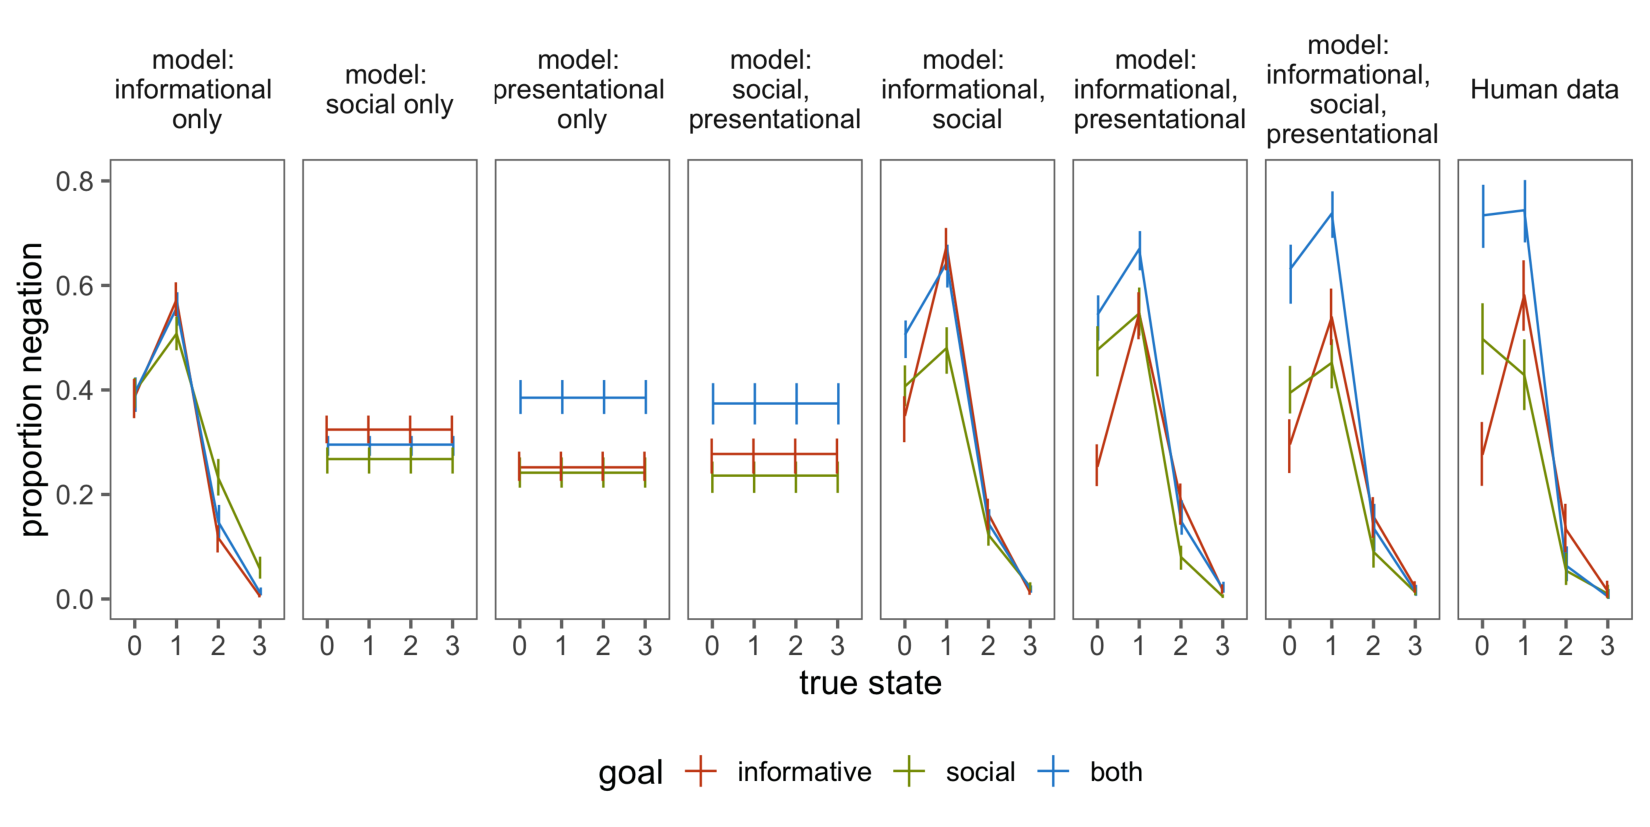
\includegraphics[width=\textwidth]{erica_yoon_dissertation_files/figure-latex/negationPlacement-1} 

}

\caption[Comparison of expected proportion of negation from model predictions and experimental results from Chapter 4.]{Experimental results (left) and fitted model predictions (right) for average proportion of negation produced among all utterances, given true states (x-axis) and goals (colors).}\label{fig:negationPlacement}
\end{figure}
\chapter*{References}\label{references}
\addcontentsline{toc}{chapter}{References}

\markboth{References}{References}

\noindent

\setlength{\parindent}{-0.20in} \setlength{\leftskip}{0.20in}
\setlength{\parskip}{8pt}

\hypertarget{refs}{}
\hypertarget{ref-airenti2011}{}
Airenti, G., \& Angeleri, R. (2011). Situation-sensitive use of
insincerity: Pathways to communication in young children. \emph{British
Journal of Developmental Psychology}, \emph{29}(4), 765--782.

\hypertarget{ref-angel2000}{}
Angel, E. (2000). \emph{Interactive computer graphics : A top-down
approach with opengl}. Boston, MA: Addison Wesley Longman.

\hypertarget{ref-angel2001}{}
Angel, E. (2001a). \emph{Batch-file computer graphics : A bottom-up
approach with quicktime}. Boston, MA: Wesley Addison Longman.

\hypertarget{ref-angel2002a}{}
Angel, E. (2001b). \emph{Test second book by angel}. Boston, MA: Wesley
Addison Longman.

\hypertarget{ref-R-ggthemes}{}
Arnold, J. B. (2017). \emph{Ggthemes: Extra themes, scales and geoms for
'ggplot2'}. Retrieved from
\url{https://CRAN.R-project.org/package=ggthemes}

\hypertarget{ref-attardo1997}{}
Attardo, S. (1997). Locutionary and perlocutionary cooperation: The
perlocutionary cooperative principle. \emph{Journal of Pragmatics},
\emph{27}(6), 753--779.

\hypertarget{ref-R-gridExtra}{}
Auguie, B. (2017). \emph{GridExtra: Miscellaneous functions for ``grid''
graphics}. Retrieved from
\url{https://CRAN.R-project.org/package=gridExtra}

\hypertarget{ref-augustine1952}{}
Augustine, S. (1952). Treaties on various issues. Washington, DC:
Catholic University of America Press.

\hypertarget{ref-R-papaja}{}
Aust, F., \& Barth, M. (2017). \emph{papaja: Create APA manuscripts with
R Markdown}. Retrieved from \url{https://github.com/crsh/papaja}

\hypertarget{ref-axia1985}{}
Axia, G., \& Baroni, M. R. (1985). Linguistic politeness at different
age levels. \emph{Child Development}, 918--927.

\hypertarget{ref-R-magrittr}{}
Bache, S. M., \& Wickham, H. (2014). \emph{Magrittr: A forward-pipe
operator for r}. Retrieved from
\url{https://CRAN.R-project.org/package=magrittr}

\hypertarget{ref-baker2017rational}{}
Baker, C. L., Jara-Ettinger, J., Saxe, R., \& Tenenbaum, J. B. (2017).
Rational quantitative attribution of beliefs, desires and percepts in
human mentalizing. \emph{Nature Human Behaviour}, \emph{1}(4), 0064.

\hypertarget{ref-baker2009action}{}
Baker, C. L., Saxe, R., \& Tenenbaum, J. B. (2009). Action understanding
as inverse planning. \emph{Cognition}, \emph{113}(3), 329--349.

\hypertarget{ref-barr2013}{}
Barr, D. J., Levy, R., Scheepers, C., \& Tily, H. J. (2013a). Random
effects structure for confirmatory hypothesis testing: Keep it maximal.
\emph{Journal of Memory and Language}, \emph{68}(3), 255--278.

\hypertarget{ref-barr2013random}{}
Barr, D. J., Levy, R., Scheepers, C., \& Tily, H. J. (2013b). Random
effects structure for confirmatory hypothesis testing: Keep it maximal.
\emph{Journal of Memory and Language}, \emph{68}(3), 255--278.

\hypertarget{ref-R-Matrix}{}
Bates, D., \& Maechler, M. (2017). \emph{Matrix: Sparse and dense matrix
classes and methods}. Retrieved from
\url{https://CRAN.R-project.org/package=Matrix}

\hypertarget{ref-R-lme4}{}
Bates, D., Mächler, M., Bolker, B., \& Walker, S. (2015). Fitting linear
mixed-effects models using lme4. \emph{Journal of Statistical Software},
\emph{67}(1), 1--48. \url{http://doi.org/10.18637/jss.v067.i01}

\hypertarget{ref-bates1976}{}
Bates, E. (1976). Acquisition of polite forms: Experimental evidence.
\emph{Language and Context: The Acquisition of Pragmatics}, 295--326.

\hypertarget{ref-bates1977}{}
Bates, E., \& Silvern, L. (1977). Social adjustment and politeness in
preschoolers. \emph{Journal of Communication}, \emph{27}(2), 104--111.

\hypertarget{ref-baxter1984}{}
Baxter, L. A. (1984). An investigation of compliance-gaining as
politeness. \emph{Human Communication Research}, \emph{10}(3), 427--456.

\hypertarget{ref-becker1986}{}
Becker, J. A. (1986). Bossy and nice requests: Children's production and
interpretation. \emph{Merrill-Palmer Quarterly (1982-)}, 393--413.

\hypertarget{ref-bernicot1991}{}
Bernicot, J. (1991). French children's conception of requesting: The
development of metapragmatic knowledge. \emph{International Journal of
Behavioral Development}, \emph{14}(3), 285--304.

\hypertarget{ref-bernicot1987}{}
Bernicot, J., \& Legros, S. (1987). Direct and indirect directives: What
do young children understand? \emph{Journal of Experimental Child
Psychology}, \emph{43}(3), 346--358.

\hypertarget{ref-bernicot2007}{}
Bernicot, J., Laval, V., \& Chaminaud, S. (2007). Nonliteral language
forms in children: In what order are they acquired in pragmatics and
metapragmatics? \emph{Journal of Pragmatics}, \emph{39}(12), 2115--2132.

\hypertarget{ref-blumkulka1987}{}
Blum-Kulka, S. (1987). Indirectness and politeness in requests: Same or
different? \emph{Journal of Pragmatics}, \emph{11}(2), 131--146.

\hypertarget{ref-blum-kulka1985}{}
Blum-Kulka, S., Danet, B., \& Gherson, R. (1985). The language of
requesting in israeli society. In \emph{Language and social situations}
(pp. 113--139). Springer.

\hypertarget{ref-bock1981}{}
Bock, J. K., \& Hornsby, M. E. (1981). The development of directives:
How children ask and tell. \emph{Journal of Child Language},
\emph{8}(01), 151--163.

\hypertarget{ref-bonnefon2006}{}
Bonnefon, J.-F., \& Villejoubert, G. (2006). Tactful or doubtful?
Expectations of politeness explain the severity bias in the
interpretation of probability phrases. \emph{Psychological Science},
\emph{17}(9), 747--751.

\hypertarget{ref-bonnefon2015}{}
Bonnefon, J.-F., Dahl, E., \& Holtgraves, T. M. (2015). Some but not all
dispreferred turn markers help to interpret scalar terms in polite
contexts. \emph{Thinking \& Reasoning}, \emph{21}(2), 230--249.

\hypertarget{ref-bonnefon2011risk}{}
Bonnefon, J.-F., Feeney, A., \& De Neys, W. (2011). The risk of polite
misunderstandings. \emph{Current Directions in Psychological Science},
\emph{20}(5), 321--324.

\hypertarget{ref-bonnefon2009}{}
Bonnefon, J.-F., Feeney, A., \& Villejoubert, G. (2009). When some is
actually all: Scalar inferences in face-threatening contexts.
\emph{Cognition}, \emph{112}(2), 249--258.

\hypertarget{ref-boyer1702}{}
Boyer, A. (1702). \emph{The english theophrastus: Or, the manners of the
age: Being the modern characters of the court, the town, and the
city...} W. Turner... R. Basset...; J. Chantry.

\hypertarget{ref-R-rwebppl}{}
Braginsky, M., Tessler, M. H., \& Hawkins, R. (n.d.). \emph{Rwebppl: R
interface to webppl}. Retrieved from
\url{https://github.com/mhtess/rwebppl}

\hypertarget{ref-R-langcog}{}
Braginsky, M., Yurovsky, D., \& Frank, M. C. (n.d.). \emph{Langcog:
Language and cognition lab things}. Retrieved from
\url{http://github.com/langcog/langcog}

\hypertarget{ref-breheny2006}{}
Breheny, R., Katsos, N., \& Williams, J. (2006). Are generalised scalar
implicatures generated by default? An on-line investigation into the
role of context in generating pragmatic inferences. \emph{Cognition},
\emph{100}(3), 434--463.

\hypertarget{ref-brown1987}{}
Brown, P., \& Levinson, S. C. (1987). \emph{Politeness: Some universals
in language usage} (Vol. 4). Cambridge university press.

\hypertarget{ref-brown1989}{}
Brown, R., \& Gilman, A. (1989). Politeness theory and shakespeare's
four major tragedies. \emph{Language in Society}, \emph{18}(2),
159--212.

\hypertarget{ref-bussey1999}{}
Bussey, K. (1999). Children's categorization and evaluation of different
types of lies and truths. \emph{Child Development}, \emph{70}(6),
1338--1347.

\hypertarget{ref-buhler1934}{}
Bühler, K. (1934). \emph{Sprachtheorie}. Oxford, England: Fischer.

\hypertarget{ref-R-brms}{}
B��rkner, P.-C. (2017). brms: An R package for bayesian multilevel
models using Stan. \emph{Journal of Statistical Software}, \emph{80}(1),
1--28. \url{http://doi.org/10.18637/jss.v080.i01}

\hypertarget{ref-clark1980}{}
Clark, H. H., \& Schunk, D. H. (1980). Polite responses to polite
requests. \emph{Cognition}, \emph{8}(2), 111--143.

\hypertarget{ref-corriveau2009}{}
Corriveau, K. H., Meints, K., \& Harris, P. L. (2009). Early tracking of
informant accuracy and inaccuracy. \emph{British Journal of
Developmental Psychology}, \emph{27}(2), 331--342.

\hypertarget{ref-corsaro1979}{}
Corsaro, W. A. (1979). Young children's conception of status and role.
\emph{Sociology of Education}, 46--59.

\hypertarget{ref-culpeper2011}{}
Culpeper, J. (2011). \emph{Impoliteness: Using language to cause
offence} (Vol. 28). Cambridge University Press.

\hypertarget{ref-R-binom}{}
Dorai-Raj, S. (2014). \emph{Binom: Binomial confidence intervals for
several parameterizations}. Retrieved from
\url{https://CRAN.R-project.org/package=binom}

\hypertarget{ref-R-Rcpp_b}{}
Eddelbuettel, D., \& Balamuta, J. J. (2017). Extending extitR with
extitC++: A Brief Introduction to extitRcpp. \emph{PeerJ Preprints},
\emph{5}, e3188v1. \url{http://doi.org/10.7287/peerj.preprints.3188v1}

\hypertarget{ref-R-Rcpp_a}{}
Eddelbuettel, D., \& François, R. (2011). Rcpp: Seamless R and C++
integration. \emph{Journal of Statistical Software}, \emph{40}(8),
1--18. \url{http://doi.org/10.18637/jss.v040.i08}

\hypertarget{ref-ervin1967}{}
Ervin-Tripp, S. M. (1967). An issei learns english. \emph{Journal of
Social Issues}, \emph{23}(2), 78--90.

\hypertarget{ref-ervin1969}{}
Ervin-Tripp, S. M. (1969). Sociolinguistics. \emph{Advances in
Experimental Social Psychology}, \emph{4}, 91--165.

\hypertarget{ref-ervin1977}{}
Ervin-Tripp, S. M. (1977). Wait for me, roller skate. In S. Ervin-Tripp
\& C. Mitchell-Kernan (Eds.), \emph{Child discourse} (pp. 165--188). New
York: Academic Press.

\hypertarget{ref-ervin1982}{}
Ervin-Tripp, S. M. (1982). Ask and it shall be given unto you:
Children's requests. \emph{Georgetown University Roundtable on Languages
and Linguistics. Contemporary Perceptions of Language: Interdisciplinary
Dimensions}, 235--245.

\hypertarget{ref-ervin1990}{}
Ervin-Tripp, S. M., Guo, J., \& Lampert, M. (1990). Politeness and
persuasion in children's control acts. \emph{Journal of Pragmatics},
\emph{14}(2), 307--331.

\hypertarget{ref-ervin1984}{}
Ervin-Tripp, S. M., O'Connor, M. C., \& Rosenberg, J. (1984). Language
and power in the family. \emph{Language and Power}, 116--135.

\hypertarget{ref-feeney2013}{}
Feeney, A., \& Bonnefon, J.-F. (2013). Politeness and honesty contribute
additively to the interpretation of scalar expressions. \emph{Journal of
Language and Social Psychology}, \emph{32}(2), 181--190.

\hypertarget{ref-finley1974}{}
Finley, G. E., \& Humphreys, C. A. (1974). Naive psychology and the
development of persuasive appeals in girls. \emph{Canadian Journal of
Behavioural Science/Revue Canadienne Des Sciences Du Comportement},
\emph{6}(1), 75.

\hypertarget{ref-fisher2002}{}
Fisher, C. (2002). The role of abstract syntactic knowledge in language
acquisition: A reply to tomasello (2000). \emph{Cognition},
\emph{82}(3), 259--278.

\hypertarget{ref-frank2012}{}
Frank, M. C., \& Goodman, N. D. (2012). Predicting pragmatic reasoning
in language games. \emph{Science}, \emph{336}(6084), 998--998.

\hypertarget{ref-franke2016}{}
Franke, M., \& Jäger, G. (2016). Probabilistic pragmatics, or why bayes'
rule is probably important for pragmatics. \emph{Zeitschrift Für
Sprachwissenschaft}, \emph{35}(1), 3--44.

\hypertarget{ref-fraser1990}{}
Fraser, B. (1990). Perspectives on politeness. \emph{Journal of
Pragmatics}, \emph{14}(2), 219--236.

\hypertarget{ref-fraser1981}{}
Fraser, B., \& Nolen, W. (1981). The association of deference with
linguistic form. \emph{International Journal of the Sociology of
Language}, \emph{1981}(27), 93--110.

\hypertarget{ref-fu2015}{}
Fu, G., Heyman, G. D., Chen, G., Liu, P., \& Lee, K. (2015). Children
trust people who lie to benefit others. \emph{Journal of Experimental
Child Psychology}, \emph{129}, 127--139.

\hypertarget{ref-gelman2006data}{}
Gelman, A., \& Hill, J. (2006). \emph{Data analysis using regression and
multilevel/hierarchical models}. Cambridge university press.

\hypertarget{ref-gleason1984}{}
Gleason, J. B., Perlmann, R. Y., \& Greif, E. B. (1984). What's the
magic word: Learning language through politeness routines?
\emph{Discourse Processes}, \emph{7}(4), 493--502.

\hypertarget{ref-goffman1967}{}
Goffman, E. (1967). \emph{Interaction ritual: Essays on face-to-face
interaction}. Aldine.

\hypertarget{ref-goodman2016}{}
Goodman, N. D., \& Frank, M. C. (2016). Pragmatic language
interpretation as probabilistic inference. \emph{Trends in Cognitive
Sciences}, \emph{20}(11), 818--829.

\hypertarget{ref-goodman2013}{}
Goodman, N. D., \& Stuhlmüller, A. (2013). Knowledge and implicature:
Modeling language understanding as social cognition. \emph{Topics in
Cognitive Science}, \emph{5}(1), 173--184.

\hypertarget{ref-dippl}{}
Goodman, N. D., \& Stuhlmüller, A. (2014). The Design and Implementation
of Probabilistic Programming Languages. \url{http://dippl.org}.

\hypertarget{ref-grice1975}{}
Grice, H. P. (1975). Logic and conversation. In P. Cole \& J. L. Morgan
(Eds.), \emph{Syntax and semantics} (Vol. 3, pp. 41--58). Academic
Press.

\hypertarget{ref-gu1990}{}
Gu, Y. (1990). Politeness phenomena in modern chinese. \emph{Journal of
Pragmatics}, \emph{14}(2), 237--257.

\hypertarget{ref-gweon2014}{}
Gweon, H., Pelton, H., Konopka, J. A., \& Schulz, L. E. (2014). Sins of
omission: Children selectively explore when teachers are
under-informative. \emph{Cognition}, \emph{132}(3), 335--341.

\hypertarget{ref-halliday1975}{}
Halliday, M. A. K. (1975). \emph{Learning how to mean: Explorations in
the development of language}. London: Edward Arnold.

\hypertarget{ref-hamlin2013mentalistic}{}
Hamlin, K. J., Ullman, T. D., Tenenbaum, J. B., Goodman, N. D., \&
Baker, C. L. (2013). The mentalistic basis of core social cognition:
Experiments in preverbal infants and a computational model.
\emph{Developmental Science}, \emph{16}(2), 209--226.

\hypertarget{ref-R-purrr}{}
Henry, L., \& Wickham, H. (2017). \emph{Purrr: Functional programming
tools}. Retrieved from \url{https://CRAN.R-project.org/package=purrr}

\hypertarget{ref-heyman2009}{}
Heyman, G. D., Sweet, M. A., \& Lee, K. (2009). Children's reasoning
about lie-telling and truth-telling in politeness contexts. \emph{Social
Development}, \emph{18}(3), 728--746.

\hypertarget{ref-hirschberg1985}{}
Hirschberg, J. B. (1985). \emph{A theory of scalar implicature}.
University of Pennsylvania.

\hypertarget{ref-R-directlabels}{}
Hocking, T. D. (2017). \emph{Directlabels: Direct labels for multicolor
plots}. Retrieved from
\url{https://CRAN.R-project.org/package=directlabels}

\hypertarget{ref-holtgraves1986}{}
Holtgraves, T. (1986). Language structure in social interaction:
Perceptions of direct and indirect speech acts and interactants who use
them. \emph{Journal of Personality and Social Psychology}, \emph{51}(2),
305.

\hypertarget{ref-holtgraves1997}{}
Holtgraves, T. (1997). YES, but... positive politeness in conversation
arguments. \emph{Journal of Language and Social Psychology},
\emph{16}(2), 222--239.

\hypertarget{ref-holtgraves1998}{}
Holtgraves, T. (1998). Interpreting indirect replies. \emph{Cognitive
Psychology}, \emph{37}(1), 1--27.

\hypertarget{ref-holtgraves2016}{}
Holtgraves, T., \& Perdew, A. (2016). Politeness and the communication
of uncertainty. \emph{Cognition}, \emph{154}, 1--10.

\hypertarget{ref-holtgraves1992}{}
Holtgraves, T., \& Yang, J.-N. (1992). Interpersonal underpinnings of
request strategies: General principles and differences due to culture
and gender. \emph{Journal of Personality and Social Psychology},
\emph{62}(2), 246.

\hypertarget{ref-huang2009a}{}
Huang, Y. T., \& Snedeker, J. (2009). Online interpretation of scalar
quantifiers: Insight into the semantics--pragmatics interface.
\emph{Cognitive Psychology}, \emph{58}(3), 376--415.
\url{http://doi.org/10.1016/j.cogpsych.2008.09.001}

\hypertarget{ref-ide1989}{}
Ide, S. (1989). Formal forms and discernment: Two neglected aspects of
universals of linguistic politeness. \emph{Multilingua-Journal of
Cross-Cultural and Interlanguage Communication}, \emph{8}(2-3),
223--248.

\hypertarget{ref-jakobson1960}{}
Jakobson, R. (1960). Linguistics and poetics. In \emph{Style in
language} (pp. 350--377). MA: MIT Press.

\hypertarget{ref-james1978}{}
James, S. L. (1978). Effect of listener age and situation on the
politeness of children's directives. \emph{Journal of Psycholinguistic
Research}, \emph{7}(4), 307--317.

\hypertarget{ref-jara2016naive}{}
Jara-Ettinger, J., Gweon, H., Schulz, L. E., \& Tenenbaum, J. B. (2016).
The naïve utility calculus: Computational principles underlying
commonsense psychology. \emph{Trends in Cognitive Sciences},
\emph{20}(8), 589--604.

\hypertarget{ref-kant1949}{}
Kant, I. (1949). On a supposed right to lie from altruistic motives.
\emph{Critical of Practical Reason and Other Writings}, 346--350.

\hypertarget{ref-kao2015}{}
Kao, J. T., \& Goodman, N. D. (2015). Let's talk (ironically) about the
weather: Modeling verbal irony. In \emph{Proceedings of the 37th annual
conference of the Cognitive Science Society}.

\hypertarget{ref-kao2014}{}
Kao, J. T., Wu, J. Y., Bergen, L., \& Goodman, N. D. (2014). Nonliteral
understanding of number words. \emph{Proceedings of the National Academy
of Sciences}, \emph{111}(33), 12002--12007.

\hypertarget{ref-kyratzis2001}{}
Kyratzis, A., \& Guo, J. (2001). Preschool girls' and boys' verbal
conflict strategies in the united states and china. \emph{Research on
Language and Social Interaction}, \emph{34}(1), 45--74.

\hypertarget{ref-lakoff1973}{}
Lakoff, R. (1973). The logic of politeness; or, minding your p's and
q's. In A. W. C. Corum T. Cedric Smith-Stark (Ed.), \emph{Papers from
the ninth regional meeting of the chicago linguistics society} (pp.
292--305). Chicago: Department of Linguistics, University of Chicago.

\hypertarget{ref-lassiter2017adjectival}{}
Lassiter, D., \& Goodman, N. D. (2017). Adjectival vagueness in a
bayesian model of interpretation. \emph{Synthese}, \emph{194}(10),
3801--3836.

\hypertarget{ref-lee2014}{}
Lee, M. D., \& Wagenmakers, E. J. (2014). \emph{Bayesian cognitive
modeling: A practical course}. Cambridge Univ. Press.

\hypertarget{ref-leech1983}{}
Leech, G. (1983). \emph{Principles of pragmatics}. London, New York:
Longman Group Ltd.

\hypertarget{ref-leichty1991}{}
Leichty, G., \& Applegate, J. L. (1991). Social-cognitive and
situational influences on the use of face-saving persuasive strategies.
\emph{Human Communication Research}, \emph{17}(3), 451--484.

\hypertarget{ref-lim1991}{}
Lim, T. S., \& Bowers, J. W. (1991). Facework: Solidarity, approbation,
and tact. \emph{Human Communication Research}, \emph{17}(3), 415--450.

\hypertarget{ref-liszkowski2008}{}
Liszkowski, U., Carpenter, M., \& Tomasello, M. (2008).
Twelve-month-olds communicate helpfully and appropriately for
knowledgeable and ignorant partners. \emph{Cognition}, \emph{108}(3),
732--739.

\hypertarget{ref-liu2017ten}{}
Liu, S., Ullman, T. D., Tenenbaum, J. B., \& Spelke, E. S. (2017).
Ten-month-old infants infer the value of goals from the costs of
actions. \emph{Science}, \emph{358}(6366), 1038--1041.

\hypertarget{ref-locher2005}{}
Locher, M. A., \& Watts, R. J. (2005). Politeness theory and relational
work. \emph{Journal of Politeness Research}, \emph{1}(1), 9--33.

\hypertarget{ref-ma2011}{}
Ma, F., Xu, F., Heyman, G. D., \& Lee, K. (2011). Chinese children's
evaluations of white lies: Weighing the consequences for recipients.
\emph{Journal of Experimental Child Psychology}, \emph{108}(2),
308--321.

\hypertarget{ref-mao1994}{}
Mao, L. R. (1994). Beyond politeness theory: ``Face'' revisited and
renewed. \emph{Journal of Pragmatics}, \emph{21}(5), 451--486.

\hypertarget{ref-matsumoto1988}{}
Matsumoto, Y. (1988). Reexamination of the universality of face:
Politeness phenomena in japanese. \emph{Journal of Pragmatics},
\emph{12}(4), 403--426.

\hypertarget{ref-R-BayesFactor}{}
Morey, R. D., \& Rouder, J. N. (2015). \emph{BayesFactor: Computation of
bayes factors for common designs}. Retrieved from
\url{https://CRAN.R-project.org/package=BayesFactor}

\hypertarget{ref-R-bindrcpp}{}
Müller, K. (2017a). \emph{Bindrcpp: An 'rcpp' interface to active
bindings}. Retrieved from
\url{https://CRAN.R-project.org/package=bindrcpp}

\hypertarget{ref-R-here}{}
Müller, K. (2017b). \emph{Here: A simpler way to find your files}.
Retrieved from \url{https://CRAN.R-project.org/package=here}

\hypertarget{ref-R-tibble}{}
Müller, K., \& Wickham, H. (2017). \emph{Tibble: Simple data frames}.
Retrieved from \url{https://CRAN.R-project.org/package=tibble}

\hypertarget{ref-R-RColorBrewer}{}
Neuwirth, E. (2014). \emph{RColorBrewer: ColorBrewer palettes}.
Retrieved from \url{https://CRAN.R-project.org/package=RColorBrewer}

\hypertarget{ref-nippold1982}{}
Nippold, M. A., Leonard, L. B., \& Anastopoulos, A. (1982). Development
in the use and understanding of polite forms in children. \emph{Journal
of Speech, Language, and Hearing Research}, \emph{25}(2), 193--202.

\hypertarget{ref-R-jsonlite}{}
Ooms, J. (2014). The jsonlite package: A practical and consistent
mapping between json data and r objects. \emph{arXiv:1403.2805
{[}Stat.CO{]}}. Retrieved from \url{https://arxiv.org/abs/1403.2805}

\hypertarget{ref-pighin2011}{}
Pighin, S., \& Bonnefon, J.-F. (2011). Facework and uncertain reasoning
in health communication. \emph{Patient Education and Counseling},
\emph{85}(2), 169--172.

\hypertarget{ref-pinker2008}{}
Pinker, S., Nowak, M. A., \& Lee, J. J. (2008). The logic of indirect
speech. \emph{Proceedings of the National Academy of Sciences},
\emph{105}(3), 833--838.

\hypertarget{ref-R-coda}{}
Plummer, M., Best, N., Cowles, K., \& Vines, K. (2006). CODA:
Convergence diagnosis and output analysis for mcmc. \emph{R News},
\emph{6}(1), 7--11. Retrieved from
\url{https://journal.r-project.org/archive/}

\hypertarget{ref-oxfordPolite}{}
Polite. (2017a). In \emph{OED online}. Oxford University Press.
Retrieved from
\url{http://www.oed.com/view/Entry/146878?rskey=4vSu4F\&result=1\&isAdvanced=false}

\hypertarget{ref-cambridgePolite}{}
Polite. (2017b). In \emph{Cambridge online dictionary}. Cambridge
University Press. Retrieved from
\url{http://dictionary.cambridge.org/us/dictionary/english/polite}

\hypertarget{ref-quinley2011}{}
Quinley, J. (2011). Politeness and trust games. \emph{Student Papers
Session, Proceedings of ESSLLI}.

\hypertarget{ref-R-base}{}
R Core Team. (2017). \emph{R: A language and environment for statistical
computing}. Vienna, Austria: R Foundation for Statistical Computing.
Retrieved from \url{https://www.R-project.org/}

\hypertarget{ref-read1978}{}
Read, B. K., \& Cherry, L. J. (1978). Preschool children's production of
directive forms. \emph{Discourse Processes}, \emph{1}(3), 233--245.

\hypertarget{ref-ryckebusch2004}{}
Ryckebusch, C., \& Marcos, H. (2004). Speech acts, social context and
parent-toddler play between the ages of 1; 5 and 2; 3. \emph{Journal of
Pragmatics}, \emph{36}(5), 883--897.

\hypertarget{ref-searle1975}{}
Searle, J. (1975). Indirect speech acts. In P. Cole \& J. L. Morgan
(Eds.), \emph{Syntax and semantics} (Vol. 3, pp. 59--82). Academic
Press.

\hypertarget{ref-shannon1948}{}
Shannon, C. E. (1948). A mathematical theory of communication.
\emph{Bell Syst. Tech. J.}, \emph{27}, 623--656.

\hypertarget{ref-shatz1973}{}
Shatz, M., \& Gelman, R. (1973). The development of communication
skills: Modifications in the speech of young children as a function of
listener. \emph{Monographs of the Society for Research in Child
Development}, 1--38.

\hypertarget{ref-snow1990}{}
Snow, C. E., Perlmann, R. Y., Gleason, J. B., \& Hooshyar, N. (1990).
Developmental perspectives on politeness:: Sources of children's
knowledge. \emph{Journal of Pragmatics}, \emph{14}(2), 289--305.

\hypertarget{ref-song2014}{}
Song, M., \& Song, H.-J. (2014). Five- to six-year-old children's
understanding of lies and truths in different contexts. \emph{The Korean
Journal of Developmental Psychology}, \emph{27}(1), 55--71.

\hypertarget{ref-spencer2000}{}
Spencer-Oatey, H. (2000). \emph{Culturally speaking: Managing rapport
through talk across cultures}. London; New York: Continuum.

\hypertarget{ref-sweetser1987}{}
Sweetser, E. (1987). The definition of lie. \emph{Cultural Models in
Language and Thought}, 43--66.

\hypertarget{ref-talwar2002}{}
Talwar, V., \& Lee, K. (2002). Development of lying to conceal a
transgression: Children's control of expressive behaviour during verbal
deception. \emph{International Journal of Behavioral Development},
\emph{26}(5), 436--444.

\hypertarget{ref-talwar2007}{}
Talwar, V., Murphy, S. M., \& Lee, K. (2007). White lie-telling in
children for politeness purposes. \emph{International Journal of
Behavioral Development}, \emph{31}(1), 1--11.

\hypertarget{ref-terkourafi2002}{}
Terkourafi, M. (2002). Politeness and formulaicity: Evidence from
cypriot greek. \emph{Journal of Greek Linguistics}, \emph{3}(1),
179--201.

\hypertarget{ref-turiel1977}{}
Turiel, E. (1977). Distinct conceptual and developmental domains: Social
convention and morality. In \emph{Nebraska symposium on motivation}.
University of Nebraska Press.

\hypertarget{ref-vanRooy2003}{}
Van Rooy, R. (2003). Being polite is a handicap: Towards a game
theoretical analysis of polite linguistic behavior. In \emph{Proceedings
of the 9th conference on theoretical aspects of rationality and
knowledge} (pp. 45--58). ACM.

\hypertarget{ref-walper1992}{}
Walper, S., \& Valtin, R. (1992). Children's understanding of white
lies. In \emph{Politeness in language: Studies in its history, theory
and practice (ed. by r.J. watts, s. ide, \& k. ehlich)} (pp. 231--251).
Mouton de Gruyter.

\hypertarget{ref-watts1989}{}
Watts, R. J. (1989). Relevance and relational work: Linguistic
politeness as politic behavior. \emph{Multilingua-Journal of
Cross-Cultural and Interlanguage Communication}, \emph{8}(2-3),
131--166.

\hypertarget{ref-watts2003}{}
Watts, R. J. (2003). \emph{Politeness}. Cambridge University Press.

\hypertarget{ref-watts1992}{}
Watts, R. J., Ide, S., \& Ehlich, K. (1992). Introduction. In
\emph{Politeness in language: Studies in its history, theory and
practice (ed. by r.J. watts, s. ide, \& k. ehlich)} (pp. 1--17). Mouton
de Gruyter.

\hypertarget{ref-wellman2004}{}
Wellman, H. M., \& Liu, D. (2004). Scaling of theory-of-mind tasks.
\emph{Child Development}, \emph{75}(2), 523--541.

\hypertarget{ref-R-ggplot2}{}
Wickham, H. (2009). \emph{Ggplot2: Elegant graphics for data analysis}.
Springer-Verlag New York. Retrieved from \url{http://ggplot2.org}

\hypertarget{ref-R-forcats}{}
Wickham, H. (2017a). \emph{Forcats: Tools for working with categorical
variables (factors)}. Retrieved from
\url{https://CRAN.R-project.org/package=forcats}

\hypertarget{ref-R-stringr}{}
Wickham, H. (2017b). \emph{Stringr: Simple, consistent wrappers for
common string operations}. Retrieved from
\url{https://CRAN.R-project.org/package=stringr}

\hypertarget{ref-R-tidyverse}{}
Wickham, H. (2017c). \emph{Tidyverse: Easily install and load the
'tidyverse'}. Retrieved from
\url{https://CRAN.R-project.org/package=tidyverse}

\hypertarget{ref-R-tidyr}{}
Wickham, H., \& Henry, L. (2017). \emph{Tidyr: Easily tidy data with
'spread()' and 'gather()' functions}. Retrieved from
\url{https://CRAN.R-project.org/package=tidyr}

\hypertarget{ref-R-dplyr}{}
Wickham, H., Francois, R., Henry, L., \& Müller, K. (2017). \emph{Dplyr:
A grammar of data manipulation}. Retrieved from
\url{https://CRAN.R-project.org/package=dplyr}

\hypertarget{ref-R-readr}{}
Wickham, H., Hester, J., \& Francois, R. (2017). \emph{Readr: Read
rectangular text data}. Retrieved from
\url{https://CRAN.R-project.org/package=readr}

\hypertarget{ref-wilson2004}{}
Wilson, G., \& Wood, K. (2004). The influence of children on parental
purchases during supermarket shopping. \emph{International Journal of
Consumer Studies}, \emph{28}(4), 329--336.

\hypertarget{ref-xu2010}{}
Xu, F., Bao, X., Fu, G., Talwar, V., \& Lee, K. (2010). Lying and
truth-telling in children: From concept to action. \emph{Child
Development}, \emph{81}(2), 581--596.

\hypertarget{ref-xu2013}{}
Xu, F., Evans, A. D., Li, C., Li, Q., Heyman, G., \& Lee, \&. K. (2013).
The role of honesty and benevolence in children's judgments of
trustworthiness. \emph{International Journal of Behavioral Development},
\emph{37}(3), 257--265.

\hypertarget{ref-yoon2019}{}
Yoon, E. J., \& Frank, M. C. (2019). Preschool children's understanding
of polite requests. In \emph{Proceedings of the forty-first annual
conference of the Cognitive Science Society}.

\hypertarget{ref-yoon2018balancing}{}
Yoon, E. J., MacDonald, K., Asaba, M., Gweon, H., \& Frank, M. C.
(2018). Balancing informational and social goals in active learning. In
\emph{Proceedings of the 40th annual conference of the cognitive science
society}.

\hypertarget{ref-yoon2017}{}
Yoon, E. J., Tessler, M. H., Goodman, N. D., \& Frank, M. C. (2017). ``I
won't lie, it wasn't amazing": Modeling polite indirect speech. In
\emph{Proceedings of the thirty-ninth annual conference of the Cognitive
Science Society}.

\hypertarget{ref-yu2011}{}
Yu, K. (2011). Culture-specific concepts of politeness: Indirectness and
politeness in english, hebrew and korean requests. \emph{Intercultural
Pragmatics}, \emph{8}(3), 385--409.


% Index?

\end{document}
